\documentclass[a4paper]{report}
\usepackage[italian]{babel}
\usepackage[latin1]{inputenc}
\usepackage[T1]{fontenc}
\usepackage[pdftex]{graphicx}
\usepackage[pdftex,colorlinks=true]{hyperref} 
\hypersetup{linkcolor=blue}
\usepackage{amssymb}
\usepackage{verbatim}

\hypersetup{ colorlinks,
  linkcolor=blue,
  filecolor=green,
  urlcolor=blue,
  citecolor=blue }

\usepackage[normalem]{ulem}

\usepackage{graphicx}
\usepackage{amssymb}
\usepackage{amsmath}
\usepackage{amsthm}
\usepackage{mathrsfs}

\newtheorem{teorema}{Teorema}
\renewcommand{\arraystretch}{2}
\newtheorem{definizione}{Definizione}
\newcommand{\bo}{\bfseries } 

\usepackage{makeidx}
\makeindex

\author{Collettivo studentesco Ingegneria Informatica Unisannio}
\title{Appunti di Sistemi}
\begin{document}
\maketitle
\setlength{\unitlength}{2cm}
	\begin{picture}(1,1)
  \put(0,0){\line(0,1){1}}
  \put(0,0){\line(1,0){1}}
  \put(0,0){\line(1,1){1}}
  \put(0,0){\line(1,2){.5}}
  \put(0,0){\line(1,3){.3333}}
  \put(0,0){\line(1,4){.25}}
  \put(0,0){\line(1,5){.2}}
  \put(0,0){\line(1,6){.1667}}
  \put(0,0){\line(2,1){1}}
  \put(0,0){\line(2,3){.6667}}
  \put(0,0){\line(2,5){.4}}
  \put(0,0){\line(3,1){1}}
  \put(0,0){\line(3,2){1}}
  \put(0,0){\line(3,4){.75}}
  \put(0,0){\line(3,5){.6}}
  \put(0,0){\line(4,1){1}}
  \put(0,0){\line(4,3){1}}
  \put(0,0){\line(4,5){.8}}
  \put(0,0){\line(5,1){1}}
  \put(0,0){\line(5,2){1}}
  \put(0,0){\line(5,3){1}}
  \put(0,0){\line(5,4){1}}
  \put(0,0){\line(5,6){.8333}}
  \put(0,0){\line(6,1){1}}
  \put(0,0){\line(6,5){1}}
\end{picture}

\section*{Prefazione}
\emph{Il presente documento \`e stato scritto con lo scopo di aiutare
  lo studente che deve affrontare l'esame di TEORIA DEI SISTEMI a ripetere
  gli argomenti trattati durante il corso, riassumendo i concetti
  fondamentali del programma. Tale documento NON deve assolutamente
  essere usato in sostituzione dei libri di testo.}
\tableofcontents

\chapter{Introduzione}

\section{Il controllo}
I \emph{problemi di controllo} hanno lo scopo di determinare le azioni
da compiere su di un processo assegnato, in modo tale che si ottenga
per esso il \emph{funzionamento desiderato}. Il processo, o
\emph{sistema sotto controllo}, \`e quell'oggetto su cui il problema
\`e posto. Il funzionamento desiderato \`e, invece, riferito al fatto
che l'andamento nel tempo delle variabili in gioco debba coincidere con
quello di altre variabili assegnate. 

Si identificano quindi: 
\begin{itemize}
\item \emph{variabili controllate}, cio\`e le grandezze di interesse;
\item \emph{segnale di riferimento}, cio\`e l'andamento desiderato
  delle variabili controllate, detto anche \emph{set-point}) nel
  caso sia un segnale costante;
\end{itemize}
Idealmente l'obiettivo di un generico problema di controllo \`e quello
di ottenere 
\begin{equation} 
  \label{eq:obiettivodiprog}
  \emph{variabile controllata} = \emph{segnale di riferimento} 
\end{equation}
Per ottenere tale risultato, si deve poter agire sul processo
attraverso le cosiddette \emph{variabili di controllo} che sono
assegnabili e manipolabili da chi effettua il controllo.
Esistono, per\`o, anche altre variabili da cui dipendono le variabili
controllate e sono i cosiddetti \emph{disturbi}, i quali non sono
manipolabili e influenzano il comportamento del processo. Dato che i
disturbi non sono noti a priori, \`e necessario definire quindi delle
incertezze. 

Bisogna ricordare che tutte le variabili che fanno parte di un
processo di controllo sono funzioni del tempo, solitamente
\emph{continuo}, ovvero descritte da una variabile reale,
convenzionalmente indicata con \textbf{t}. 

L'andamento della variabile di controllo \`e determinato da un organo
detto \emph{controllore} o \emph{regolatore}. In particolare l'insieme 
\framebox{processo + controllore} forma il \emph{sistema di controllo}.

\section{Specifiche di progetto}
Dalla relazione \ref{eq:obiettivodiprog} si evince che, essendo essa
una relazione \textit{ideale}, \`e di fatto irraggiungibile. Nella
realt\`a la relazione \ref{eq:obiettivodiprog} diventa: 
\begin{equation}\label{eq:obiettivoreale}
  \emph{variabile controllata}  \simeq \emph{segnale di riferimento}
\end{equation} 
e, introducendo l'\emph{errore} del sistema, abbiamo:
\begin{equation}\label{eq:deferrore}
  \emph{errore}  = \emph{segnale di riferimento} - \emph{variabile controllata}
\end{equation}
L'obiettivo, quindi, \`e quello di minimizzare quanto pi\`u possibile
l'errore in tutte le condizioni di funzionamento di interesse tenendo
conto dei vincoli sul valore minimo e massimo della variabile di
controllo per evitare eccessive sollecitazioni sul processo. 

\section{Controllo Feedforward e Feedback}
Un'importante classificazione del controllo \`e quella effettuata in base alle informazioni possedute dal regolatore (da non confondere con quelle del progettista del controllore). Tale classificazione definisce:
\begin{description}
\item[Controllo Feedforward]{\emph{(o controllo in anello aperto o ad
    azione diretta)}}: quando il controllore possiede informazioni
  solo sul segnale di riferimento ed eventualmente sul disturbo
  (figura \ref{fig:fig1})
\begin{figure}[!h]
  \begin{center}
    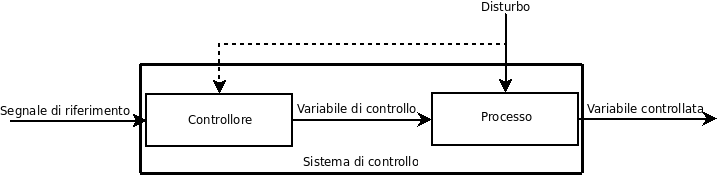
\includegraphics[scale=0.5]{./figures/feedforward.png}
    \caption{Feedforward Control}
    \label{fig:fig1}
  \end{center}
\end{figure}
\item[Controllo Feedback]{\emph{(o controllo in anello chiuso o in
    retroazione o feedback)}} (figura \ref{fig:fig2}): quando il
  controllore ha a disposizione anche la variabile controllata. 
\begin{figure}[!h]
  \begin{center}
    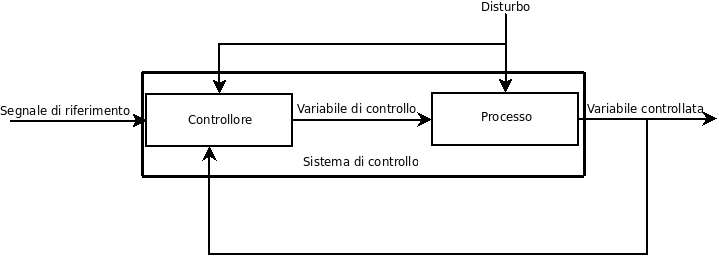
\includegraphics[scale=0.5]{./figures/feedback.png}\caption{Feedback Control}\label{fig:fig2}
  \end{center}
\end{figure}  
\end{description}
In particolare, nel controllo retroazionato, si vede che l'azione di
controllo impressa al processo in $t = \bar t$, dipende anche dalla
variabile controllata per $ t \leq \bar t$.

\section{Modelli matematici}
Al fine di affrontare nel modo giusto un problema di controllo, \`e
molto conveniente studiarlo prima in termini puramente
matematici. Ci\`o vuol dire che tutte le specifiche di
progetto (sull'errore e sul controllo) devono essere espresse in
termini formali ed inoltre \`e necessario disporre anche di una
descrizione matematica degli elementi che compaiono nel sistema di
controllo. Il modello matematico \`e, dunque, un insieme di relazioni matematiche
quali equazioni algebriche, differenziali, etc., che descrivono il
sistema di controllo formalizzando le variabili che interconnettono i
singoli componenti. 

{\em Un sistema ha infiniti modelli. Un modello rappresenta infiniti
  sistemi.}

\chapter{Sistemi dinamici a tempo continuo}
\section{Concetti fondamentali}
\subsection{Variabili di ingresso, stato e uscita}
Un sistema dinamico a tempo continuo \`e un modello
matematico di un oggetto fisico che interagisce con il mondo che lo
circonda attraverso due vettori di variabili dipendenti dal tempo $t$: 
\begin{itemize}
\item{\emph{variabili di ingresso}}: sono le azioni che vengono
  compiute sull'oggetto in esame da agenti esterni che ne influenzano
  il comportamento;
\item{\emph{variabili di uscita}}: \`e quanto del comportamento
  dell'oggetto stesso \`e di interesse. 
\end{itemize}
In particolare esiste un rapporto di \emph{causa-effetto} tra le
variabili di ingresso e quelle di uscita. Un sistema dinamico a tempo
continuo \`e schematizzato in figura \ref{fig:fig3}.
\begin{figure}[!h]
  \begin{center}
    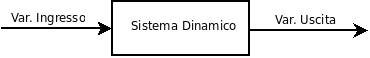
\includegraphics[scale=0.5]{./figures/dynasys.png}
    \caption{Sistema Dinamico}\label{fig:fig3}
  \end{center}
\end{figure}  

\subsection{Rappresentazione I-S-U}
Formalizzando la definizione di sistema dinamico a tempo continuo
abbiamo le seguenti equazioni:
\begin{equation}\label{eq:eqstato}
  \dot{x}(t)=f(x(t),u(t),t)
\end{equation}
\begin{equation}\label{eq:eqout}
  y=g(x(t),u(t),t)
\end{equation}
che formano la cosiddetta \emph {rappresentazione I-S-U
  (Ingresso-Stato-Uscita)} o pi\`u semplicemente
\emph{rappresentazione di stato} del sistema.
L'equazione \ref{eq:eqstato} \`e la \emph{equazione di stato},
mentre la \ref{eq:eqout} \`e la \emph{trasformazione
  d'uscita}. Il numero \textbf{n} delle variabili di stato di un
sistema definisce l'\emph{ordine} del sistema. In figura
\ref{fig:fig4} \`e schematizzato un sistema dinamico a tempo continuo
con la sua equazione di stato e trasformazione d'uscita.
\begin{figure}[!h]
  \begin{center}
    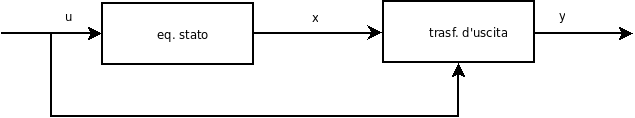
\includegraphics[scale=0.5]{./figures/dynaeq.png}
    \caption{Sistema dinamico con equazioni di stato e trasformazione
      d'uscita}
    \label{fig:fig4}
  \end{center}
\end{figure} 

L'equazione di stato mette in relazione con l'ingresso le variabili
che descrivono la situazione interna del sistema, mentre la
trasformazione di uscita, sulla base di tale situazione e
dell'ingresso applicato in uno specifico istante \textbf{t}, consente
di determinare l'uscita all'istante \textbf{t}. 
% Per gli esempi consultare il testo di riferimento \cite{FCA} 

Nello scegliere le variabili di stato di un sistema, bisogna tener
conto che esse ci aiutano a capire quanto sia necessario conoscere
della situazione interna o della \emph{storia passata} del sistema per
poter calcolare l'uscita. 

Nei sistemi fisici, la situazione interna \`e generalmente definita da
accumuli di energia, quantit\`a di moto, massa e, quindi, pu\`o essere
opportuno scegliere come variabili di stato quelle da cui queste
grandezze dipendono. Ad esempio:
\begin{itemize}
\item nei sistemi elettrici \`e conveniente utilizzare come variabili
  di stato le tensioni dei condensatori o le correnti degli induttori,
  perch\`e da queste dipendono gli accumuli di energia elettrica e magnetica;
\item nei sistemi meccanici \`e utile usare, invece, posizione e
  velocit\`a come variabili di stato, perch\`e legate ad accumuli di
  energia potenziale, quantit\`a di moto ed energia cinetica;
\item nei sistemi termodinamici si possono usare come variabili di
  stato le temperature, perch\`e da esse dipendono le energie termiche
  immagazzinate.
\end{itemize}

\subsection{Classificazione dei sistemi}
I sistemi possono essere: 
\begin{itemize}
\item[**]{\textbf {Sistemi monovariabili e multivariabili (SISO e
    MIMO)}}: i sistemi SISO (\emph{Single Input Single Output}) sono
  dotati di una sola variabile di ingresso ed una sola variabile
  d'uscita; i sistemi MIMO (\emph{Multiple Input Multiple Output})
  sono gli altri.
\item[**]{\textbf{Sistemi propri, strettamente propri e non
    dinamici}}: in generale un sistema si dice \emph{proprio} quando
  il legame ingresso-uscita \`e di tipo differenziale. In questo caso,
  il tempo ha un'importanza notevole, poich\`e la relazione tra $x$ e
  $y$ non \`e immediata.

  Nei sistemi propri, per conoscere il valore dell'uscita occorre
  sapere necessariamente due informazioni: 
  \begin{itemize}
  \item la condizione iniziale, cio\`e il valore dell'uscita in un
    istante prefissato;
  \item l'insieme dei valori che l'ingresso assume all'istante di osservazione.
  \end{itemize}
  Per questo motivo, i sistemi propri vengono definiti {\em sistemi con
  memoria}, poich\`e l'uscita in un determinato istante $t$ dipende
  sia dal valore dell'ingresso in quell'instante sia da quanto \`e
  successo in precedenza; se,
  invece, la trasformazione d'uscita pu\`o essere espressa nella forma
  \begin{equation}\label{eq:eqstrpr}
    y(t) = g(x(t),t)
  \end{equation}
  ovvero se l'uscita dipende solo dallo stato e non dall'ingresso, allora il
  sistema si dice \emph{strettamente proprio}\index{Sistema
    strettamente proprio} o \emph{puramente dinamico}\index{Sistema
    puramente dinamico}; se, infine, l'uscita \`e nella forma
  \begin{equation}\label{eq:eqstaticsys}
    y(t) = g(u(t),t)
  \end{equation} ovvero se l'uscita dipende solo dall'ingresso e non c'\`e
  alcuno stato, allora il sistema \`e un particolare sistema proprio
  detto \emph{sistema non dinamico o statico}\index{Sistema non
    dinamico}\index{Sistema statico}.
\item[**]{\textbf{Sistemi invarianti e varianti nel tempo}}
Nel caso in cui le funzioni $f$ e $g$ non dipendano esplicitamente dal
tempo, allora il sistema si dice \emph{invariante nel tempo} o
\emph{stazionario}. In particolare si ha: 
\begin{equation}\label{eq:ltisys}
  \dot{x}(t) = f(x(t),u(t))
\end{equation}
\begin{equation}\label{eq:ltisys2}
  y(t)=g(x(t),u(t))
\end{equation}
Invece, se anche una sola delle funzioni $f$ e $g$ dipende
esplicitamente da $t$, il sistema si dice \emph{variante nel tempo} ed
in questo caso le equazioni del sistema sono le gi\`a note
\ref{eq:eqstato} e \ref{eq:eqout}.

\item[**]{\textbf{Sistemi lineari e non lineari}}: se le equazioni del
  sistema sono combinazioni lineari delle varie
componenti dei vettori $x(t)$ e $u(t)$, allora il sistema si dice
\emph{lineare}, altrimenti \`e \emph{non lineare}. La rappresentazione
I-S-U, espressa in forma matriciale, del generico sistema lineare
tempo invariante (LTI) \`e la seguente: 
\begin{equation}\label{eq:matltisys}
  \dot{x}(t)=Ax(t)+Bu(t)
\end{equation}
\begin{equation}
  y(t)=Cx(t)+Du(t)
\end{equation}
dove:
\begin{itemize}
\item {A \`e detta \emph{matrice della dinamica}. La sua dimensione
  \`e $[n \times n]$, dove n \`e il numero di variabili di
  stato}~\footnote{N.B. Se il sistema \`e T.V.(Tempo Variante) allora
  le matrici sono funzioni del tempo};
\item{B \`e la \emph{matrice degli ingressi}. La sua dimensione \`e
  $[n\times m]$, dove m \`e il numero degli ingressi};
\item{C \`e la \emph{matrice delle uscite}. Dimensionalmente \`e
  $[p\times n]$, dove p \`e il numero di uscite};
\item{D \`e la \emph{matrice di trasmissione}. Vale zero se
  non esiste un legame ingresso-uscita. La sua dimensione \`e
  $[p\times m]$}.
\end{itemize}
\end{itemize}

\section{Risposta impulsiva}
L'impulso \`e un artificio matematico usato per rappresentare segnali
brevi, ma intensi. In particolare si definisce l'\emph{impulso di
  Dirac} come:
\begin{displaymath}
\textrm{imp(t)}=\delta(t) = \left\{ \begin{array}{ll}
 1 & \textrm{if $t=0$}\\
 0 & \textrm{if $t\neq0$}\\
  \end{array} \right.
\end{displaymath}
Le sue propriet\`a sono:
\begin{enumerate}
\item {$P_\varepsilon(t)\ge 0$}
\item {$P_\varepsilon(t)=0$} all'esterno di [0,$\varepsilon$]
\item{$\int_{0}^{\varepsilon}P_\varepsilon(\tau) d\tau=1$} ha area
  unitaria $\forall \varepsilon$ 
\item{$\delta(t)\triangleq  \lim_{\varepsilon \rightarrow \infty}
  P_\varepsilon(t) $} 
\item{$\int_{-\infty}^{+\infty}\delta(t)dt=1$}
\item {$\int_{-\infty}^{+\infty}\delta(t)f(t)dt=f(0)$ Campionamento}
\end{enumerate}

\textsl{Se al sistema applichiamo un impulso, esso risponder\`a con i
  suoi \textbf{MODI NATURALI}}. 
\subsection{Risposta impulsiva del sistema}
In generale:
\begin{equation}
  Y_F(s)=G(s)U(s)\label{eq:eqlaprispf}
\end{equation}
se 
$$u(t)=\delta(t) \Rightarrow Y_F(s)=G(s)\cdot 1\Rightarrow
Y_F(s)=G(s) \stackrel
{{\mathfrak{L^{-1}}}}{\longrightarrow}\protect
g(t)=y_f(t)$$ 
con $\mathfrak{L}^{-1}$ pari all'\emph{Antitrasformata di Laplace}
(vedere Appendice \ref{apx:laplace})\\
\textbf{La risposta impulsiva \`e:}
\begin{equation}\label{eq:eqpulseresp}
  \protect\mathfrak{L}^{-1}[G(s)\mathfrak{L}(\delta(t)]
\end{equation}

\section{Equilibrio e punti di equilibrio}
Prendendo in considerazione i sistemi stazionari ed applicando ad essi
ingressi costanti, indicati come $u(t) = \bar{u}(t)$, si hanno
movimenti dello stato e dell'uscita anch'essi costanti nel
tempo. Questi movimenti costanti sono detti rispettivamente {\em
  stati} ed \emph{uscite di equilibrio}.

Per definizione: "Uno stato di equilibrio (o \emph{steady
  state})\index{Stato di equilibrio}\index{Steady state} \`e 
uno stato in cui un sistema, sollecitato da un ingresso costante, in
un qualunque istante di tempo, permane in questo stato
indefinitamente"~\footnote{Se il sistema da solo va in posizione di
  equilibrio, allora il punto di equilibrio \`e detto
  \emph{attrattivo}\index{Punto di equilibrio attrattivo} e il sistema
  \`e asintoticamente stabile} ovvero, se in $\bar{t}$ il sistema si
trova nello stato $x(\bar{t})=\bar{x}$, allora $\forall t >\bar{t}$,
il sistema si trover\`a nello stesso stato $x(t)=\bar{x}$.

In termini matematici, gli stati di equilibrio devono soddisfare
l'equazione $\dot{x}(t)=0$, cio\`e sono le soluzioni $\bar{x}$
costanti nel tempo dell'equazione: 
\begin{equation}\label{eq:eqsteady}
  f(\bar{x},\bar{u})=0
\end{equation}
A ciascuna delle soluzioni (se ne esistono), corrisponde un'uscita di
equilibrio $\bar{y}$, calcolabile mediante la relazione 
\begin{equation}\label{eq:outsteady}
  \bar{y}=g(\bar{x},\bar{u})
\end{equation}
In particolare, gli stati di equilibrio $\bar{x}$ sono le soluzioni
dell'equazione: 
\begin{equation}
  A\bar{x}+B\bar{u} = 0
\end{equation}
e ad ogni stato di equilibrio corrisponde un'uscita di equilibrio:
\begin{equation}
  \bar{y}=C\bar{x}+D\bar{u}
\end{equation}

\subsection{La matrice $A$}
La matrice $A$ \`e detta matrice della dinamica\index{Matrice della
  dinamica}\index{Matrice Jacobiana}\index{Jacobiano}, matrice
Jacobiana o Jacobiano. Ha dimensioni $n \times n$, con $n$ grado del sistema e numero
di variabili di stato. Se $A$ \`e invertibile, cio\`e se $det(A) \neq
0$, lo stato di equilibrio \`e:
\[
  \begin{array}{l}
    \bar{x} = -A^{-1} B \bar{u}\\
    \bar{y} = ( -C A^{-1} B + D) \bar{u}
  \end{array}
\]
La matrice $[D - CA^{-1} B]$ \`e il {\bf guadagno
  statico}\index{Guadagno statico}, una costante che rappresenta il
rapporto tra uscita ed ingresso a regime, quando, cio\`e, il
transitorio \`e esaurito. Se $det(A) = 0$ 
\[
  A \bar{x} + B \bar{u} = 0
\]
ammette infinite soluzioni o nessuna soluzione. Ci\`o implica infiniti
possibili stati di equilibrio o nessuno stato di equilibrio. In questo
caso la nozione di guadagno statico perde senso.

\section{Stabilit\`a}
Il criterio di stabilit\`a fu introdotto dal matematico
\href{http://it.wikipedia.org/wiki/Aleksandr_Michajlovi\%C4\%8D_Ljapunov}{Liapunov}. Liapunov
considerava che ``piccole'' perturbazioni dello stato
iniziale, rispetto ad un valore di riferimento, provocano solo ``piccole''
perturbazioni del movimento dello stato, che si annulleranno
eventualmente su tempi lunghi. 

\subsection{Stabilit\`a dell'equilibrio}
Si considera un sistema dinamico T.I. con ingresso costante
$u(t)=\bar{u}$, con $t \ge 0$, e un corrispondente stato di equilibrio
$\bar{x}$ detto \emph{nominale}. Inoltre si considera anche un
movimento dello stato $x(t)$, detto \emph{perturbato}, generato a
partire da $\bar{u}$ e da uno stato iniziale $x_0$.

Possiamo affermare che: \emph{"Uno stato di equilibrio si dice stabile
  se, ad una perturbazione arbitrariamente piccola, il movimento
  perturbato rimane ``vicino'' all'equilibrio nominale. \`E instabile
  se si ha un allontanamento dello stato del sistema dall'equilibrio
  stesso"}.

Definito ``polo dominante''\index{Polo dominante} come il polo che si
trova pi\`u a destra degli altri, di seguito mostriamo la tabella che
riassume i tipi di sistemi classificati secondo la stabilit\`a: 

\begin{table}[hbp!]
  \begin{center}
    \begin{tabular}[hbp!]{|c|p{5cm}|}
      \hline
      \multicolumn{2}{|c|}{STABILITA'} \\
      \hline
      \hline
      TIPO & Definizione \\
      \hline
      \hline
      \hline
      ASINTOTICAMENTE STABILE & Tutti i MODI NATURALI sono
      convergenti, ovvero tutti i poli sono a sinistra (il \emph{polo
        dominante} \`e a sinistra)\\ 
      \hline
      MARGINALMENTE STABILE & Non esistono modi naturali divergenti, ma ne
      esiste uno, o pi\`u di uno, limitato che non tende a $0$, ovvero il polo
      dominante \`e sull'asse immaginario \\ 
      \hline
      INSTABILE & Esiste un modo divergente, ovvero il polo dominante
      \`e a destra\\
      \hline
      DEBOLMENTE INSTABILE & Non esistono modi divergenti esponenziali, ma
      ne esiste uno divergente ``debolmente'' (ad esempio, potenze della
      $t$ che crescono pi\`u lentamente dell'esponenziale), ovvero il polo \`e
      sull'asse immaginario con molteplicit\`a maggiore di $1$.\\
      \hline
    \end{tabular}
    \caption{Stabilit\`a dei sistemi}
    \label{tab:tab1}
  \end{center}
\end{table}

\chapter{Sistemi LTI a tempo continuo}
\section{Evoluzione di un sistema}
Nei movimenti dello stato e dell'uscita di un sistema, si pu\`o
individuare un contributo dipendente solo dallo stato iniziale e uno
dipendente solo dall'ingresso. 

\begin{description}
\item[Evoluzione libera]\index{Evoluzione libera} (o movimenti
liberi) \`e il contributo al movimento dello stato e dell'uscita
funzione solo dello stato iniziale, ovvero quello che, a parit\`a di
stato iniziale, si avrebbe se l'ingresso fosse nullo. 
\item[Evoluzione forzata]\index{Evoluzione forzata} \`e il contributo
funzione solo dell'ingresso, ovvero quello che si avrebbe se, a parit\`a
di ingresso, lo stato iniziale fosse nullo. 
\end{description}
Il sistema LTI (Lineare Tempo Invariante) a tempo continuo \`e descritto
dalle equazioni \ref{eq:matltisys}. In questa sezione vengono
presentati due schemi riassuntivi che descrivono i modi di tali
sistemi con autovalori distinti e doppi.

La rappresentazione grafica viene effettuata sul piano
complesso\index{Piano complesso} o piano di Gauss\index{Piano di
  Gauss}. Il piano di Gauss pu\`o essere pensato come un piano
cartesiano modificato affinch\`e l'asse $x$ rappresenti la parte reale
({\em asse reale}) e l'asse $y$ rappresenti la parte immaginaria ({\em
asse immaginario}) di un numero complesso. Nel nostro caso il piano di
Gauss ci consentir\`a di avere una localizzazione chiara dei vari tipi
di poli dei nostri sistemi.

\section{Sistema del primo ordine}
L'evoluzione libera di un sistema del primo ordine ha un andamento di
tipo esponenziale: 
\[
y(t) = e^{\lambda t}
\]
Tale esponenziale, \`e convergente se $\lambda < 0$ , costante se
$\lambda = 0$, divergente se $\lambda > 0$.

\section{Sistema del secondo ordine}
\subsubsection{Poli distinti}
\begin{figure}[!h]
  \begin{center}
    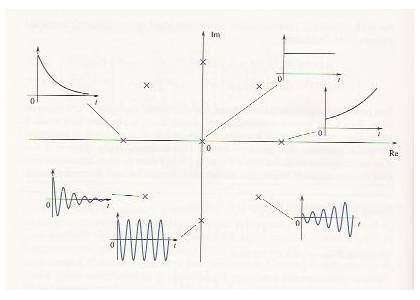
\includegraphics[scale=0.7]{./figures/modisingol.png}
    \caption{Modi dei sistemi con autovalori distinti}\label{fig:modising}
  \end{center}
\end{figure} 
La figura \ref{fig:modising} mostra l'andamento dei modi naturali, o
risposta impulsiva, dei sistemi del secondo ordine, secondo il tipo di
poli del sistema.

\begin{description}
\item[A] Il polo dominante \`e a sinistra dell'asse immaginaria,
  cio\`e \`e a parte reale negativa e parte immaginaria
  nulla. Il sistema \`e asintoticamente stabile. L'andamento della
  funzione di uscita \`e di tipo esponenziale negativo:
  \[
  y_l(t) = k_1 e^{at} + k_2 e^{bt}
  \]
\item[B] Il polo dominante \`e complesso a parte reale negativa. Il sistema \`e
  asintoticamente stabile. L'andamento \`e una sinusoide di ampiezza
  sempre minore. La funzione di uscita \`e
  \[
  y_l(t) = k_1 e^{\alpha t}sin(\omega t) + k_2 e^{\alpha t}cos(\omega t)
  \]
  con $\alpha < 0$: l'oscillazione \`e convergente;
\item[C] Il polo dominante si trova nell'origine degli assi. Il
  sistema \`e marginalmente stabile. La funzione di uscita \`e pari a
  $y_l(t) = k_1 e^{at} + k_2 e^{bt}$. Se consideriamo $a = 0$, la
  funzione sar\`a una semiretta costante di ordinata $k_1$;
\item[D] Il polo dominante \`e complesso a parte reale nulla. Il
  sistema \`e marginalmente stabile. La funzione \`e una sinusoide
  costante, a media nulla;
\item[E] Il polo dominante \`e complesso a parte reale positiva. Il
  sistema \`e instabile; diverge come una sinusoide di ampiezza sempre
  maggiore. La funzione di uscita \`e
  \[
  y_l(t) = k_1 e^{\alpha t}sin(\omega t) + k_2 e^{\alpha t}cos(\omega t)
  \]
  con $\alpha > 0$.
\item[F] Il polo dominante ha parte reale positiva. Il sistema \`e
  instabile. La funzione \`e un esponenziale positivo.
\end{description}

Nota: nel caso di poli complessi, la risposta in evoluzione libera
pu\`o anche  porsi nella forma:
\[
y_l(t) = A e^{\alpha t} sin(\omega t + \beta)
\]
dove
\[
A = \sqrt{k^2_1 + k^2_2}
\]
\[
\beta = arctan \dfrac{k_2}{k_1}
\]

\subsubsection{Poli doppi}
\begin{figure}[!h]
  \begin{center}
    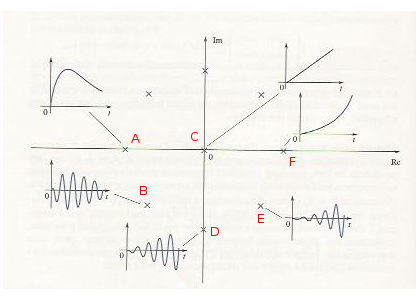
\includegraphics[scale=0.7]{./figures/modidoppi.png}
    \caption{Modi dei sistemi con autovalori doppi}\label{fig:modidop}
  \end{center}
\end{figure}
La figura \ref{fig:modidop} mostra l'andamento dei modi naturali, o
risposta impulsiva, dei sistemi del secondo ordine, secondo il tipo di
poli del sistema.

\begin{description}
\item[A] I poli sono a parte reale negativa. La funzione presenta una
  sovraelongazione prima di convergere;
\item[B] I poli sono complessi a parte reale negativa. Il sistema \`e
  asintoticamente stabile. L'andamento \`e una sinusoide di ampiezza
  sempre minore;
\item[C] I poli giacciono nell'origine degli assi. Il sistema \`e
  instabile. La funzione diverge con una pendenza inferiore ad un
  esponenziale, ma diverge;
\item[D - E] I poli sono complessi a parte reale nulla o positiva. In
  entrabi i casi, il sistema \`e instabile e la funzione \`e una
  sinusoide di ampiezza sempre maggiore;
\item[F] I poli sono reali a parte reale positiva. Il sistema \`e
  instabile. La funzione diverge esponenzialmente.
\end{description}

Nel caso dei modi con autovalori doppi, notiamo che le funzioni
partono dall'origine degli assi. Questo comportamento \`e facilmente
dimostrabile analizzando la risposta al gradino di sistemi del secondo
ordine con poli coincidenti. Risolvendo la risposta al gradino per $t
= 0$
\[
y(t) = \mu \left(1 - e^{- \frac{t}{T}} - \dfrac{t}{T}e^{- \frac{t}{T}}\right)
\]
notiamo che il punto di partenza \`e effettivamente lo
zero. Calcolandone la derivata prima, otteniamo la pendenza. Con la
derivata seconda, si ottiene la concavit\`a e la convessit\`a.

\section{Criteri di stabilit\`a}
In un sistema stazionario lineare, la determinazione delle propriet\`a
di stabilit\`a dipende solo dal movimento libero. Inoltre, anche il
calcolo del movimento libero pu\`o essere evitato in quanto \`e possibile
verificare condizioni di asintotica stabilit\`a e instabilit\`a,
valutando esclusivamente gli autovalori del sistema. Nell'appendice
\ref{apx:jacob} viene mostrato come valutare la stabilit\`a dei punti
di equilibrio di un sistema, attraverso il calcolo della matrice
\textsl{Jacobiana}. 
Seguono tre importanti teoremi sulla stabilit\`a dei sistemi:
\newtheorem{Th1}{Teorema}[section]
\newtheorem{Th2}[Th1]{Teorema}
\newtheorem{Th3}[Th1]{Teorema}
\newtheorem{Th4}[Th1]{Teorema}
 
\begin{Th1}\label{th:th1}
  Lo stato di equilibrio di un sistema lineare stazionario \`e stabile,
  asintoticamente stabile o instabile se e solo se tutti gli stati di
  equilibrio del sistema sono rispettivamente stabili, asintoticamente
  stabili o instabili. 
\end{Th1}

\begin{Th2}\label{th:th2}
  Un sistema lineare stazionario \`e stabile se e solo se tutti i
  movimenti liberi dello stato sono limitati, cio\`e non vanno
  all'infinito, per tutte le $t \geq 0$ e per tutti gli stati iniziali;
  \`e asintoticamente stabile se e solo se tutti i movimenti liberi dello
  stato sono tendenti a zero per $t \to \infty$; \`e instabile se e solo
  se almeno un movimento libero dello stato \`e divergente (ovvero non
  limitato).
\end{Th2}

\begin{Th3}\label{th:th3}
  Un sistema lineare stazionario \`e asintoticamente stabile se e solo
  se tutti i suoi autovalori hanno parte reale negativa ($\Re<0$).
\end{Th3}

\begin{Th4}\label{th:th4}
  Un sistema lineare stazionario \`e instabile se e solo se almeno uno
  dei suoi autovalori ha parte reale positiva ($\Re>0$).
\end{Th4}

\subsubsection{Propriet\`a dei sistemi asintoticamente stabili}
\begin{itemize}
\item Il movimento asintotico coincide con quello forzato, visto che
  il movimento libero tende ad annullarsi;
\item La risposta all'impulso tende a zero, poich\`e coincide con un
  movimento libero;
\item La risposta ad un qualunque ingresso di durata limitata tende a
  zero in modo asintotico;
\item Lo stato e l'uscita di equilibrio conseguenti ad un qualunque
  ingresso $u(t) = \bar{u}$ sono unici.
\end{itemize}

\subsection{Teorema di Routh}\label{pg:routh}\index{Teorema di Routh}
Il metodo utilizzato per valutare la stabilit\`a asintotica di un
sistema senza calcolare la sua evoluzione libera, cio\`e senza la
risoluzione di un'equazione differenziale, \`e quello definito
attraverso l'applicazione del \textsl{Teorema di Routh}.
Il Teorema di Routh prende in considerazione gli autovalori di un
sistema e ne valuta il segno. In particolare si utilizza il
\emph{polinomio caratteristico} nel dominio di Laplace:~\footnote{Vedere Appendice \ref{apx:laplace}}
\begin{equation}\label{eq:polycarat}
  \varphi(s)=det(sI-A)=s^n+p_1s^{n-1}+p_2s^{n-2}+\ldots+p_{n-1}s+p_n
\end{equation}
dove $n$ \`e il grado dell'equazione polinomiale e si considera l'\emph{equazione caratteristica}:
\begin{displaymath}
  \varphi(s)=0
\end{displaymath}

Applicando il teorema ~\ref{th:th3}, si pu\`o valutare l'asintotica
stabilit\`a valutando i coefficienti del polinomio
caratteristico~\ref{eq:polycarat} scritto in forma pi\`u generale:
\begin{equation}\label{eq:polycaratgen}
  \varphi(s)=\varphi_0 s^n+\varphi_1s^{n-1}+\varphi_2s^{n-2}+\ldots+\varphi_{n-1}s+\varphi_n ~con ~\varphi_0 \ne 0
\end{equation}

Si osservi inoltre che
\begin{equation}\label{eq:phigen}
  \varphi(s)=\varphi_0 \prod_{i=1}^{n}(s-s_i)
\end{equation}
per cui, se il sistema \`e asintoticamente stabile,
risulta $$\sum_{i=1}^n s_i < 0$$

\newtheorem{Th5}{Teorema}[section]
\begin{Th5}\label{th:th5}
  Se il sistema ~\ref{eq:matltisys} \`e asintoticamente stabile
  $\Rightarrow$ i coefficienti $\varphi_i$, $i=0,1,\ldots,n$, del
  polinomio caratteristico ~\ref{eq:polycarat} sono concordi, ovvero
  hanno tutti lo stesso segno.
\end{Th5}
A dimostrazione del teorema ~\ref{th:th5} si pu\`o imporre nella
~\ref{eq:phigen} la condizione
\begin{displaymath}
  \Re (s_i) < 0
\end{displaymath}

\subsubsection{Applicazione del Teorema di Routh}
Attraverso la definizione della cosiddetta {\em tabella di Routh},
\`e possibile formulare una condizione necessaria e sufficiente di
asintotica stabilit\`a. 
Tale tabella si costruisce a partire dal polinomio
caratteristico~\ref{eq:polycarat} ed ha $n + 1$ righe e una struttura
triangolare: ogni $2$ righe (eccetto la prima se $n$ \`e
pari), il numero di elementi (colonne) diminuisce di 1. 
In particolare la tabella si costruisce come segue:\\
\begin{center}
  \begin{tabular}{|r|l|}
    \hline
    potenze & coefficienti\\
    \hline
    n &
    $\varphi_0  ~\varphi_2 ~\varphi_4 ~\ldots ~\ldots$\\
    n-1 &
    $\varphi_1 ~\varphi_3  ~ \varphi_5  \ldots~\ldots$\\n-2 &
    $a_1 ~a_2 ~a_3 ~\ldots$\\
    n-3&
    $b_1 ~b_2 ~b_3 ~\ldots$\\
    n-4&
    $c_1 ~c_2 ~c_3 ~..$\\
    \ldots &\ldots ~\ldots\\
    1 &\ldots ~..\\
    0 & \ldots
  \end{tabular}
\end{center}
Le prime due righe contengono i coefficienti del polinomio
caratteristico in ordine, fino all'esaurimento. Successivamente i
coefficienti $a$, $b$ e $c$ si calcolano in base agli elementi delle
righe che li precedono, ovvero:
\begin{equation}
  a_1=-\frac{1}{\varphi_1}det\left(\left[
    \begin{array}{cc}
      \varphi_0 & \varphi_{2} \\
      \varphi_1&\varphi_{3}
    \end{array}
    \right]\right)
\end{equation}
\begin{equation}
  a_2=-\frac{1}{\varphi_1}det\left(\left[
    \begin{array}{cc}
      \varphi_0 & \varphi_4 \\
      \varphi_1 &\varphi_5
    \end{array}
    \right]\right)
\end{equation}
\begin{center}
  \begin{displaymath}
    \vdots
  \end{displaymath}
\end{center}
\begin{equation}
  b_1=-\frac{1}{a_1}det\left(\left[
    \begin{array}{cc}
      \varphi_1 & \varphi_3 \\
      a_1 &a_2
    \end{array}
    \right]\right)
\end{equation}
\begin{equation}
  b_2=-\frac{1}{a_1}det\left(\left[
    \begin{array}{cc}
      \varphi_1 & \varphi_5 \\
      a_1 &a_3
    \end{array}
    \right]\right)
\end{equation}
\begin{center}
  \begin{displaymath}
    \vdots
  \end{displaymath}
\end{center}
\begin{equation}
  c_1=-\frac{1}{b_1}det\left(\left[
    \begin{array}{cc}
      a_1 & a_2 \\
      b_1 &b_2
    \end{array}
    \right]\right)
\end{equation}
\begin{equation}
  c_2=-\frac{1}{b1_1}det\left(\left[
    \begin{array}{cc}
      a_1 & a_3 \\
      b_1 &b_3
    \end{array}
    \right]\right)
\end{equation}
\begin{center}
  \begin{displaymath}
    \vdots
  \end{displaymath}
\end{center}

Dopo aver effettuato tali calcoli si pu\`o affermare che:
\newtheorem{Th6}{Teorema}[section]
\begin{Th6}\label{th:routh}
Il sistema ~\ref{eq:matltisys} \`e asintoticamente stabile
se la tabella di Routh \`e ben definita e tutti gli elementi
della prima colonna sono di segno concorde. 
Il numero di radici nel semipiano a parte reale positiva \`e pari ai
cambiamenti di segno presenti nella prima colonna dell matrice di
Routh.
\end{Th6}
Una tabella di Routh \`e ``ben definita'' se tra gli elementi della
prima colonna non \`e presente alcuno zero. Per approfondimenti vedere
l'appendice ~\ref{apx:stabil}.

Se ne ricava che, supposto il coefficiente $\phi_0 > 0$ della equazione
\ref{eq:polycarat}, condizione necessaria e sufficiente perch\`e tutte
le radici nella \ref{eq:polycarat} siano a parte reale negativa \`e
che tutti i coefficienti della prima colonna della tabella di Routh
siano positivi. 

\section{Linearizzazione}
Prendiamo in considerazione un generico sistema MIMO, non lineare,
T.I. e proprio, descritto dalle equazioni precedentemente esposte
(\ref{eq:ltisys}) e sollecitato da un ingresso costante $u(t)=\bar{u}$. \\
Si fa poi riferimento al suo stato di equilibrio, ovvero quello stato
per cui vale l'identit\`a:
\begin{equation}
  0 = f(\bar{x},\bar{u})~\footnote{La dipendenza dal tempo \`e implicita,
    per cui la variabile \emph{t} pu\`o essere omessa}
\end{equation} a cui corrisponde l'uscita di equilibrio:
\begin{equation}
  \bar{y}=g(\bar{x},\bar{u})
\end{equation}
Il procedimento della \emph{linearizzazione} consiste nel descrivere
il comportamento di un sistema NL (Non Lineare) attorno al suo punto
di equilibrio nominale, approssimandolo ad un sistema lineare.
Pertanto si pone:
\begin{eqnarray}
  u(t)=\bar{u}+\delta u(t)\\
  x(t)=\bar{x}+\delta x(t)\\
  y(t)=\bar{y}+\delta y(t)\\
  x_{t_0}=\bar{x}+\delta x_{t_0}
\end{eqnarray}
dove $\delta u(t)$, $\delta x(t)$, $\delta y(t)$ e $\delta x_{t_0}$
rappresentano le variazioni (scostamenti) di $ u, x, y $ e dello stato
$x_{t_0}$. Con queste considerazioni, le equazioni \ref{eq:ltisys} e
\ref{eq:ltisys2} diventano:  
\begin{equation}\label{eq:linstate}
  \dot{\bar{x}}+\delta \dot{x}(t)=f(\bar{x}+\delta x(t),\bar{u} +\delta u(t))
\end{equation}
\begin{equation}\label{eq:linout}
  \bar{y}+\delta y(t)=g(\bar{x}+\delta x(t), \bar{u}+\delta u(t))
\end{equation} assumendo come condizione iniziale:
\begin{equation}\label{eq:lincondin}
  \bar{x}+\delta x(t_0)=\bar{x}+\delta x_{t_0}
\end{equation}
Ricordiamo che la ``serie di Taylor''\index{Serie di Taylor} di una
funzione $f$, definita in un intervallo aperto e derivabile infinite
volte, \`e espressa come una serie di potenze:
\begin{equation}\label{eq:serieDiTaylor}
  T(x) = \sum_{n=0}^{\infty} \dfrac{f^{(n)}(a)}{n!} (x - a)^n
\end{equation}
dove $f^{(n)}a$ \`e la derivata ennesima di $f$ valutata in $a$, ossia
la derivata parziale ennesima di $f$.
Sviluppando in serie di Taylor e troncando lo sviluppo al primo termine otteniamo:
\begin{equation}\label{eq:statetaylor}
  \delta \dot{x}(t)=f(\bar{x},\bar{u})+\frac{\partial f(x,u)}{\partial
    x} \Bigg |_{x=\bar{x},u=\bar{u}}\delta x(t)+\frac{\partial
    f(x,u)}{\partial u} \Bigg |_{x=\bar{x},u=\bar{u}}\delta u(t)
\end{equation}
\begin{equation}\label{eq:outtaylor}
  \bar{y}+\delta y(t)=g(\bar{x},\bar{u})+\frac{\partial
    g(x,u)}{\partial x} \Bigg |_{x=\bar{x},u=\bar{u}}\delta
  x(t)+\frac{\partial g(x,u)}{\partial u} \Bigg
  |_{x=\bar{x},u=\bar{u}}\delta u(t) 
\end{equation}
Combinando le \ref{eq:statetaylor} e \ref{eq:outtaylor} con le
\ref{eq:linstate}, \ref{eq:linout} e \ref{eq:lincondin} si ha : 
\begin{eqnarray}\label{eq:linsys}
  \left\{ \begin{array}{l}
    \delta \dot{x}(t)=A \delta x(t) + B \delta u(t)\\
    \delta y(t)=C \delta x(t) + \delta u(t)\\
    \delta x((t_0)=\delta x_{t_0}
  \end{array}\right.
\end{eqnarray}
dove:
\begin{eqnarray}\label{eq:linmatr}
  A=\frac{\partial f(x,u)}{\partial x} \Bigg |_{x=\bar{x},u=\bar{u}}\\
  B=\frac{\partial f(x,u)}{\partial u} \Bigg |_{x=\bar{x},u=\bar{u}}\\
  C=\frac{\partial g(x,u)}{\partial x }\Bigg |_{x=\bar{x},u=\bar{u}}\\
  D=\frac{\partial g(x,u)}{\partial u} \Bigg |_{x=\bar{x},u=\bar{u}}
\end{eqnarray}
In particolare, prendendo ad esempio un sistema del secondo ordine,
ovvero con due stati $x_1$ e $x_2$, avente le  matrici dimensionate
come segue: 
A[2x2], B[1x2], C[2x1] e D=0 e caratterizzato dalla seguente
rappresentazione ISU: 
\begin{equation}
  \left\{ \begin{array}{l}
    \dot{x_1}=f_1(x_1,x_2,u)\\
    \dot{x_2}=f_2(x_1,x_2,u)\\
    y=g(x_1, x_2, u)
  \end{array}\right.
\end{equation}
 
Le matrici del modello linearizzato (\ref{eq:linsys}) si calcolano in
questo modo: 
\begin{displaymath}\label{eq:matrix}
\mathbf{A} =
\left( \begin{array}{cc}
\frac{\partial f_1(x_1,x_2,u)}{\partial x_1}  & \frac{\partial f_1(x_1,x_2.u)}{\partial x_2} \\
\frac{\partial f_2(x_1,x_2.u)}{\partial x_1}  & \frac{\partial f_2(x_1,x_2,u)}{\partial x_2} \\
\end{array} \right)\Bigg |_{x_1=\bar{x_1},x_2=\bar{x_2},u=\bar{u}}\\
\end{displaymath}
\begin{displaymath}
\mathbf{B} =
\left( \begin{array}{c}
\frac{\partial f_1(x_1,x_2,u)}{\partial u}\\
\frac{\partial f_2(x_1,x_2.u)}{\partial u} 
\end{array} \right)\Bigg |_{x_1=\bar{x_1},x_2=\bar{x_2},u=\bar{u}}
\end{displaymath}
\begin{displaymath}
\mathbf{C} =
\left( \begin{array}{cc}
\frac{\partial g(x_1,x_2,u)}{\partial x_1}  & \frac{\partial g(x_1,x_2.u)}{\partial x_2} \\
\end{array} \right)\Bigg |_{x_1=\bar{x_1},x_2=\bar{x_2},u=\bar{u}}
\end{displaymath}

Abbiamo cos\`i ottenuto un sistema lineare e stazionario che lega le
variabili prime delle variabili in gioco che prende il nome di {\em
  sistema linearizzato} e che \`e di fondamentale importanza per
descrivere in maniera approssimata il comportamento del sistema in
esame attorno al punto di equilibrio stabile considerato, tenendo
presenti le sufficientemente piccole variazioni degli ingressi
($\delta{u}$) e dello stato iniziale ($\delta{x_{t0}}$) e delle
conseguenti variazioni dello stato ($\delta{x}$) e dell'uscita
($\delta{y}$).

\subsection{Stabilit\`a dell'equilibrio}
\begin{teorema}
  Lo stato di equilibrio $\bar{x}$, relativo all'ingresso $\bar{u}$, di un
  sistema non lineare risulta asintoticamente stabile se tutti gli
  autovalori del sistema linearizzato hanno parte reale negativa.
\end{teorema}
Va da se che si pu\`o evitare il calcolo degli autovalori e limitarsi a
valutare il polinomio caratteristico, sulla base del Teorema \ref{th:routh}.

%% FUNZIONE DI TRASFERIMENTO
\chapter{Funzione di Trasferimento}
\`E una nuova rappresentazione dei sistemi dimanici a tempo continuo
lineari e stazionari. Essa mette in relazione tra loro le trasformate
di Laplace delle variabili di ingresso e di uscita.

\section{Definizione della funzione di trasferimento}
Si considera il sistema \ref{eq:matltisys}. Applicando le
trasformate di Laplace (vedi appendice \ref{apx:laplace}) ad ambo i
membri si ha: 
\begin{displaymath}
  sX(s) - x(0) = AX(s) + BU(s)
\end{displaymath}
\begin{displaymath}
  Y(s) = CX(s) + DU(s)
\end{displaymath}
Proseguendo:
\[
  sX(s) - AX(s) = BU(s) + x(0)
\]
Per mettere in evidenza $X(s)$, dobbiamo moltiplicare $s$ per la
matrice identit\`a: \`e impossibile sottrarre la matrice $A$ allo
scalare $s$.
\[
  X(s)(SI - A) = BU(s) + x(0)
\]
Iterando, si ottengono le seguenti equazioni: 
\begin{eqnarray}\label{eq:tdlstateout}
  X(s)=\underbrace{(sI-A)^{-1}BU(s)}_{\mathfrak{L}\{Risposta \; forzata\}} +
  \underbrace{(sI-A)^{-1}x(0)}_{\mathfrak{L}\{Risposta \; libera\}}\\
  Y(s)=\underbrace{(C(sI-A)^{-1}B+D)U(s)}_{\mathfrak{L}\{Risposta \;
      forzata\}} +
  \underbrace{C(sI-A)^{-1}x(0)}_{\mathfrak{L}\{Risposta \; libera\}}
\end{eqnarray}
che rappresentano le trasformate di Laplace del movimento dello stato
e dell'uscita. In particolare, considerando le condizioni iniziali nulle si ha:
\begin{equation}\label{eq:transfout}
  Y(s)=G(s)U(s)
\end{equation}
Si definisce pertanto:
\begin{equation}\label{eq:fdt}
  G(s) \triangleq (C(sI-A)^{-1}B+D) \qquad
  \textrm{\emph{funzione/matrice di trasferimento}} 
\end{equation}
Effettuando l'antitrasformazione di Laplace (appendice
\ref{apx:laplace}) della \ref{eq:transfout}, si pu\`o conoscere il
movimento forzato $y_f$ che, nel caso di stato iniziale nullo,
coincide con il movimento d'uscita $y$.

Nel caso di sistemi SISO, se
$u(t)=\delta(t) \stackrel{\mathfrak{L}}{\Rightarrow} U(s)=1$ allora
\[
Y(s)=G(s)
\]
ovvero si pu\`o interpretare la funzione di trasferimento come la
trasformata di Laplace della risposta impulsiva (\ref{eq:eqpulseresp}). 

\subsection{Struttura della funzione di trasferimento}
In generale la \ref{eq:fdt} \`e una funzione razionale in $s$ data dal
rapporto di due polinomi ovvero: 
\begin{equation}\label{eq:genfdt}
  G(s)=\frac{N(s)}{D(s)}=\frac{\beta_\nu s^\nu+\beta_{\nu-1}s^{\nu-1}+
    \ldots+\beta_1s+\beta_0}{\alpha_\nu s^\nu+\alpha_{\nu-1}s^{\nu-1}+
    \ldots+\alpha_1s+\alpha_0}
\end{equation} 
Senza perdita di generalit\`a, si pu\`o considerare $D(s)$ come
polinomio monico, cio\`e $\alpha_\nu=1$.

\begin{itemize}
\item Se il sistema \`e strettamente proprio\index{Sistema
  strettamente proprio}, allora il grado del
  denominatore $D(s)$ sar\`a maggiore  del grado del numeratore $N(s)$.
\item Se il sistema \`e proprio\index{Sistema proprio}, allora il
  grado del denominatore $D(s)$ sar\`a pari al grado del numeratore
  $N(s)$. 
\item Per i sistemi impropri\index{Sistema improprio} il grado del
  numeratore $N(s)$ sar\`a maggiore del grado del denominatore $D(s)$.
\end{itemize}
La differenza tra il grado di $D(s)$ e quello di $N(s)$ \`e detta
\emph{\textbf{grado relativo}}\index{Grado relativo} ed indica la
\emph{prontezza del sistema}.

\subsubsection{Poli e zeri}
Le \emph{singolarit\`a} di un sistema \`e l'insieme dei \textbf{poli} e
degli \textbf{zeri}. Per definizione:
\begin{description}
\item[Poli] sono i valori che annullano il denominatore $D(s)$. Essi
  sono anche le radici dell'equazione $det(sI - A) = 0$, cio\`e sono gli
  autovalori del sistema;
\item[Zeri] sono i valori che annullano il numeratore $N(s)$.
\end{description}

\subsection{Relazione tra funzione di trasferimento ed equazioni
  differenziali} 
Considerando un sistema rappresentato dall'equazione differenziale:
\begin{displaymath}
  \frac{d^n y(t)}{dt^n}+\alpha_{n-1}\frac{d^{n-1} y(t)}{dt^{n-1}} +
  \ldots+\alpha_{1}\frac{dy(t)}{dt} + \alpha_0y(t)=
\end{displaymath}\label{eq:gendiffsys}
\begin{equation}
  =\beta_n\frac{d^n u(t)}{dt^n} + \beta_{n-1}\frac{d^{n-1}
    u(t)}{dt^{n-1}} + \ldots+\beta_{1}\frac{du(t)}{dt}+\beta_0u(t)
\end{equation}
ed effettuando per ambo i membri la trasformata di Laplace, tenendo
conto delle sue propriet\`a di derivazione, ed imponendo 
\begin{displaymath}
  y(0)=0 ~, \qquad \frac{d^iy(0)}{dt^i}=0 ~, \qquad i=1,2,\ldots,n-1
\end{displaymath}
si ha:
\begin{displaymath}
  s^nY(s)+\alpha_{n-1}s^{n-1}Y(s)+\ldots+\alpha_1sY(s)+\alpha_0Y(s)=
\end{displaymath}
\begin{equation}\label{eq:lapgendiffsys}
  = \beta_n s^nU(s)+\beta_{n-1}s^{n-1}U(s)+\ldots+\beta_1sU(s)+\beta_0U(s)
\end{equation}
da cui
\begin{equation}\label{eq:secgenfdt}
  \frac{Y(s)}{U(s)}=G(s)\triangleq \frac{\beta_n
    s^n+\beta_{n-1}s^{n-1} +
    \ldots+\beta_1s+\beta_0}{s^n+\alpha_{n-1}s^{n-1} + \ldots+\alpha_1s+\alpha_0}
\end{equation}

\subsection{Cancellazioni e stabilit\`a}
Quando valutiamo la $G(s)$, pu\`o capitare che ci siano radici comuni
tra numeratore e denominatore. Questa eventualit\`a pu\`o portarci nello
scenario in cui il numero di poli $v$ sia minore del numero degli $n$
autovalori del polinomio. Com'\`e noto la $G(s)$, nota anche come
rappresentazione esterna, descrive il legame tra l'ingresso e l'uscita
del sistema. Questo ci porta a considerare che gli autovalori che non
coincidono con i poli di $G(s)$ siano associati a parti ``nascoste''
del sistema. In questo caso, gli autovalori potrebbero perfino avere
parte reale positiva.

In definitva, per assicurarci che il polinomio caratteristico descriva
adeguatamente il sistema e ci garantisca l'asintotica stabilit\`a,
dobbiamo accertarci dell'assenza di cancellazioni di radici. Quando
nel calcolo della $G(s)$ non avvengono semplificazioni, il
denominatore coincide con il polinomio caratteristico ed i poli
coincidono con gli autovalori: la sola conoscenza dei poli \`e
sufficiente ad accertare la stabilit\`a del sistema.

\subsection{Ritardo di tempo}
\begin{equation}\label{eq:ritardoDiTempo}
  y(t) = u(t - \tau)
\end{equation}
L'equazione \ref{eq:ritardoDiTempo} descrive il ritardo di tempo, un
sistema lineare stazionario. Applicando la trasformata di Laplace ad
entrabi i membri otteniamo:
\[
  Y(s) = e^{- \tau s} U(s)
\]
che ci porta alla seguente funzione di trasferimento:
\[
  G(s) = e^{- \tau s}
\]
Se essa \`e moltiplicata per una generica funzione di trasferimento
$G'(s)$, le valutazioni si spostano su quest'ultima e solo alla fine
si applica la traslazione ai risultati ottenuti.

\section{Parametri della funzione dei trasferimento e sue rappresentazioni}
Molto spesso \`e conveniente rappresentare la G(s) di un sistema SISO in
uno di questi due modi:
\begin{equation}\label{eq:firstformfdt}
  G(s)=\dfrac{\rho \prod_i(s+z_i) \prod_i(s^2+2 \zeta_i \alpha_{ni}s +
    \alpha^{2}_{ni})}{s^g \prod_i(s+p_i) \prod_i(s^2+2 \xi_i
    \omega_{ni}s + \omega^2_{ni})}
\end{equation}
\begin{equation}\label{eq:secformfdt}
  G(s)= \dfrac{\mu \prod_i(1 + \tau_i s) \prod_i\left(1+\dfrac{2 \zeta_i
      s}{\alpha_{ni}} + \dfrac{s^2}{\alpha^{2}_{ni}}\right)}{s^g
    \prod_i (1+T_i s) \prod_i\left(1+\dfrac{2 \xi_i s} {\omega_{ni}} +
    \dfrac{s^2}{\omega^2_{ni}}\right)}
\end{equation}
Nelle equazioni \ref{eq:firstformfdt} e ~\ref{eq:secformfdt} si identificano:
\begin{itemize}
\item $\rho$ = \emph{costante di trasferimento}
\item $g$ = \emph{tipo} del sistema. In particolare
  \framebox{$g=(poli-zeri) \; nell'origine$}
\item $z_i$ e $p_i$ sono rispettivamente gli zeri ed i poli $\neq$ 0
  cambiati di segno
\item $\alpha_{ni}>0$ e $\omega_{ni}>0$ sono le \emph{pulsazioni
  naturali} rispettivamente degli zeri e dei poli complessi e coniugati.
\item $\zeta_i$ (``zita'') e $\xi_i$ (``x\`i'')(in modulo $< 1$), sono gli \emph{smorzamenti}
  rispettivamente degli zeri e dei poli complessi e coniugati.
\item $\mu$ \`e il \emph{guadagno}
\item $\tau_i$ e $T_i$ sono le \emph{costanti di tempo} ($\neq 0$) che
  per definizione coincidono con il reciproco cambiato di segno dei
  poli e degli zeri $\neq 0$
\end{itemize}
Combinando le due equazioni \ref{eq:firstformfdt} e
~\ref{eq:secformfdt} si pu\`o facilmente verificare che:
\begin{eqnarray}\label{eq:fdtparms}
  \mu=\dfrac{\rho \prod_iz_i\prod_i\alpha_{ni}^2}{\prod_ip_i\prod_i\omega^2_{ni}}\\
  \rho=\dfrac{\mu\prod_i\tau_i\prod_i\omega_{ni}^2}{\prod_iT_i\prod_i\alpha^2_{ni}}\\
  \tau_i=\dfrac{1}{z_i}\\
  T_i=\dfrac{1}{p_i}
\end{eqnarray}

\section{Il guadagno}
Si consideri un sistema con la funzione di trasferimento descritta
dalla \ref{eq:secformfdt}. Inoltre si supponga che esso sia
asintoticamente stabile, quindi $g \le 0$, $T_i > 0$, $\xi_i > 0$. Si
consideri il caso particolare in cui $g = 0$ e vi sia un ingresso
$u(t) = \bar{u}$ la cui trasformata di Laplace \`e
$U(s) = \dfrac{\bar u}{s}$.

Il teorema del valore finale\index{Teorema del valore finale}
(\ref{teoremaValoreFinale}) permette 
di calcolare il valore costante a regime di una funzione temporale,
data la sua trasformata di Laplace. Esso pu\`o essere correttamente
applicato solo se tutti i poli sono a sinistra dell'asse immaginario
ed un solo polo \`e nell'origine. In questo caso, il valore sar\`a una
costante diversa da zero. Se non ci sono poli nell'origine il valore
finale sar\`a zero. Se ci sono poli positivi, il valore finale \`e
indefinito: il sistema diverge.
\begin{equation}\label{eq:teoremaDelValoreFinale}
  \lim_{t \rightarrow \infty} f(t) = \lim_{s \rightarrow 0} s F(s)
\end{equation}

Calcolando la risposta di regime applicando il teorema del valore
finale, si ha:
\begin{displaymath}
  \bar y=\lim_{t \to \infty}y(t)=\lim_{s \to 0}sG(s)\dfrac{\bar u}{s}
  = \lim_{s \to 0}s(C(sI-A)^{-1}B+D)\dfrac{\bar u}{s}=
\end{displaymath}
\begin{equation}\label{eq:firstgain}
  =G(0)\bar u=(-CA^{-1}B+D)\bar u
\end{equation}
e per la \ref{eq:secformfdt} si ha:
\begin{equation}\label{eq:secgain}
  \bar y=\lim_{s \to 0}sG(s)\frac{\bar u}{s}=\mu \bar u
\end{equation}
Confrontando le due equazioni \ref{eq:firstgain}, ~\ref{eq:secgain}
risulta che:
\begin{equation}\label{eq:defgain}
  \mu = G(0) = -CA^{-1}B + D
\end{equation}
$\mu$ \`e il guadagno che in questo caso coincide con il guadagno
statico (per $g = 0$). Il guadagno statico si calcola valutando
$G(s)\Big|_{s=0}$. Il guadagno, quindi, \`e \emph{il rapporto tra
  uscita e ingresso}. Considerando la differenza tra i poli
nell'origine e gli zeri nell'origine $g$, nel caso in cui $g \ne 0$,
$\mu$ viene chiamato \emph{guadagno generalizzato}\index{Guadagno
  generalizzato} e si calcola come: 
\begin{equation}\label{eq:gengain}
  \mu=\lim_{s \to 0} s^g G(s)
\end{equation}

/!$\backslash$ in questo caso $\mu$ non \`e pi\`u il guadagno statico!

Una considerazione importante da fare \`e che i poli ``rallentano'' mentre
gli zeri ``accelerano'' per quanto riguarda l'evoluzione della risposta di
un sistema. In particolare, tornando alle costanti di tempo, si pu\`o dire
che quelle al denominatore $D(s)$ sono legate alla velocit\`a con cui si
esauriscono i transitori del sistema: maggiore \`e il valore di
una costante di tempo, pi\`u lentamente si esaurir\`a il contributo
sull'uscita dato dal polo corrispondente.

In conclusione, possiamo affermare che $y_{\infty}$ \`e nullo nel caso
di $g < 0$ (presenza di azioni derivative), altrimenti \`e pari al
guadagno $\mu$.

\section{Pulsazione naturale e smorzamento}\label{par:pulsazsmorz}
Note le equazioni \ref{eq:firstformfdt} e \ref{eq:secformfdt}, si
consideri una coppia di poli complessi e coniugati (o analogamente, di
zeri complessi e coniugati) $a \pm jb$ definiti come radici
dell'equazione $s^2 + 2\xi \omega_ns + \omega^2_n = 0$. Si definiscono:
\begin{eqnarray}
a=-\xi\omega_n\\
b=\omega_n\sqrt{1-\xi^2}
\end{eqnarray}
Quindi il modulo dei poli \`e la pulsazione naturale
$\omega_n$\index{Pulsazione naturale}, mentre
lo smorzamento $\xi$\index{Smorzamento} \`e il $\cos \theta$, dove
$\theta$ \`e l'angolo compreso tra la congiungente i poli con
l'origine e il semiasse reale negativo. 
\begin{figure}[!h]
  \begin{center}
    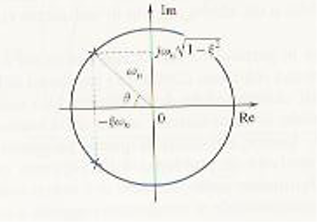
\includegraphics[scale=0.5]{./figures/complconj.png}
    \caption{Parametri dei poli complessi e coniugati}\label{fig:complparms}
  \end{center}
\end{figure}
Pertanto, tenendo fisso $\omega_n$, al variare di $\xi$ da $-1$ a $+1$
($cos \theta$ con $\theta = \pi$ o $\theta = 0$), i poli si spostanto
su una circonferenza di raggio $\omega_n$ centrata nell'origine. La
tabella \ref{tab:tabsmorz} mostra la posizione dei poli al variare
dello smorzamento $\xi$.
\begin{table}[!h]
\begin{center}
\begin{tabular}{c|c}
\hline
$\xi=0$ & poli immaginari puri in $s = \pm j\omega_n$\\
$\xi>0$ & poli a parte reale negativa\\
$\xi<0$ & poli a parte reale positiva\\
$\xi=1$ & poli reali coincidenti in $s = -\omega_n$\\
$\xi=-1$ & poli reali coincidenti in $s = \omega_n$\\
\hline
\end{tabular}
\caption{Posizione dei poli al variare dello smorzamento $\xi$}
\label{tab:tabsmorz}
\end{center}
\end{table}

\section{Risposta al gradino}
Per modellare un'improvvisa commutazione del valore dell'ingresso ed
analizzare il comportamento del sistema a tale variazione, si studia
il movimento dell'uscita in risposta al gradino. Il gradino che
prenderemo in considerazione si suppone di ampiezza unitaria, in
quanto per la propriet\`a della linearit\`a, la risposta al gradino di
ampiezza $\bar{u}$ \`e semplicemente data da quella del gradino unitario
moltiplicata per $\bar{u}$.

\subsection{Considerazioni sul valore iniziale e finale}
Per un sistema avente funzione di trasferimento pari a:
\begin{equation}
  G(s)=\dfrac{\beta_ms^m+\beta_{m-1}s^{m-1}+\ldots+\beta_0}{\alpha_ns^n
    + \alpha_{n-1}s^{n-1}+\ldots+\alpha_0}
\end{equation}
con $m \le n$, il valore iniziale della risposta al gradino, pu\`o
essere calcolato con il teorema del valore iniziale:
\begin{equation}\label{eq:teoremaDelValoreIniziale}
  \lim_{s \to \infty} sF(s) = f(0)
\end{equation}
che permette di determinare il valore asintotico iniziale della
funzione partendo dalla sua trasformata. Otteniamo quindi:
\begin{displaymath}
  y(0)=\lim_{s \to \infty}
  s\underbrace{\frac{\beta_ms^m+\beta_{m-1}s^{m-1}+\ldots+\beta_0}{\alpha_ns^n+\alpha_{n-1}
      s^{n-1}+\ldots+\alpha_0}\dfrac{1}{s}}_{\textsl{Risposta al
      gradino}} = \left\{ \begin{array}{ll}0 & m < n
    \\ \dfrac{\beta_n}{\alpha_n} & m = n\end{array}\right.
\end{displaymath}
Possiamo iterare il teorema del valore iniziale anche per le derivate
successive del valore iniziale, ricordando le regole di derivazione
della trasformata di Laplace (\ref{apx:laplace}).\\
Ad esempio, se $m < n$ e $y(0) = 0$ si ha:
\begin{displaymath}
  \dot{y}(0)=\lim_{s \to \infty}s(sY(s)-y(0))=
\end{displaymath}
\begin{displaymath}
  =\lim_{s \to \infty}s^2\dfrac{\beta_ms^m+\beta_{m-1}s^{m-1} +
    \ldots+\beta_0}{\alpha_ns^n +
    \alpha_{n-1}s^{n-1}+\ldots+\alpha_0}\frac{1}{s} =
  \left\{ \begin{array}{ll}0 & m<n-1 \\
    \dfrac{\beta_n}{\alpha_n} & m=n-1\end{array}\right.
\end{displaymath}
In generale, per $m < n$, sono nulle le prime ($n-m-1$) derivate di
$y$ in $t = 0$.

\subsection{Parametri della risposta al gradino}
I parametri caratterizzanti la risposta al gradino sono:
\begin{description}
\item[valore di regime~$y_\infty$] \hfill \\
  valore dell'uscita a transitorio esaurito:
  \begin{itemize}
  \item se $g = 0$ esso \`e pari a $\mu$; 
  \item se $g < 0$ esso \`e 0;
  \end{itemize}
\item[valore massimo~$y_{max}$]\hfill \\
  massimo valore assunto dall'uscita;
\item[sovraelongazione massima percentuale] $S\%$ \hfill \\
  ampiezza, in \%, della sovraelongazione massima rispetto a
  $y_\infty$, cio\`e
  \begin{displaymath}
    S\% = 100 \cdot \dfrac{y_{max}-y_\infty}{y_\infty}
  \end{displaymath}
\item[tempo di massima sovraelongazione~$T_M$] \hfill \\
  primo istante in cui $y = y_{max}$;
\item[tempo di salita $T_s$] \hfill \\
  tempo richiesto affinch\`e l'uscita passi dal 10\% al 90\% del suo
  valore di regime;
\item[tempo di ritardo o tempo all'emivalore $T_r$] \hfill \\ tempo
  necessario affinch\`e l'uscita raggiunga un valore pari a 0.5 volte
  $y_\infty$; 
\item[tempo di assestamento~$T_{a\varepsilon}$] \hfill \\
  tempo necessario affinch\`e il modulo della differenza tra l'uscita
  e il valore di regime
  $y_\infty$ rimanga definitivamente al di sotto di $\varepsilon\%$
  ovvero l'uscita sia compresa nell'intervallo
  $[(1-0.01\varepsilon)y_\infty,(1+0.01\varepsilon)y_\infty]$. Ad
  esempio con ``tempo al 99\%'', indicato con $T_{a1}$, si far\`a
  riferimento al tempo necessario affinch\`e l'uscita entri
  definitivamente nella fascia di ampiezza $\pm 0.01 y_\infty$. In
  generale si dir\`a che $T_{a\varepsilon}$ \`e il \emph{``tempo di
    assestamento al ($100-\varepsilon$)\%''}.
  Nota: un fenomeno si considera esaurito se raggiunge l'$1\%$ del
  valore iniziale (esponenziale decrescente a zero) o se raggiunge il
  $99\%$ del valore a regime (esponenziale convergente crescente).
\item[periodo di oscillazione $T_p$] \hfill \\
  distanza temporale tra i primi due massimi dell'uscita.
\end{description}

\begin{figure}[!h]
  \begin{center}
    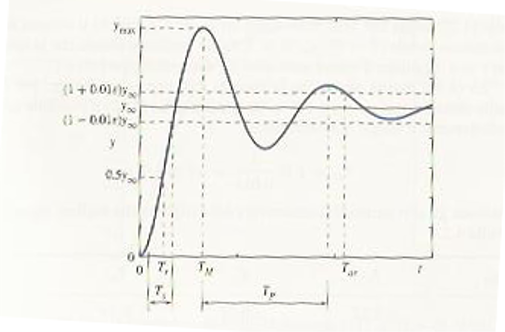
\includegraphics[scale=0.5]{./figures/parms.png}
    \caption{Parametri della risposta al gradino}\label{fig:caratparms}
  \end{center}
\end{figure} 

\section {Sistemi del $I�$ ordine}
Un sistema del primo ordine \`e caratterizzato dalla seguente funzione
di trasferimento:
\begin{equation}\label{eq:firstordfdt}
  G(s) = \dfrac{\mu}{1+sT}
\end{equation}
Calcolando la risposta al gradino:
\begin{displaymath}
  Y(s) = G(s)\dfrac{1}{s} = \dfrac{\mu}{(1+sT)s}
\end{displaymath}
Determiniamo l'antitrasformata (Appendice \ref{apx:laplace}) $y(t)$
sfruttando la teoria dei fratti semplici:
\[
  \dfrac{\mu}{(1 + sT)s} = \dfrac{A}{s} + \dfrac{B}{(1 + sT)}
\]
Moltiplichiamo ambo i membri per $s$:
\[
  \dfrac{\mu s}{(1 + sT)s} = A + \dfrac{Bs}{(1 + sT)}
\]
Facciamo tendere $s$ alla radice del denominatore di $A$, quindi a
zero.
\[
  A = \mu
\]
Per calcolare $B$, moltiplichiamo entrambi i membri per $(1 + sT)$:
\[
  \dfrac{\mu}{(1 + sT)s} \cdot (1 + sT) = \dfrac{A(1 + sT)}{s} + B
\]
Facciamo tendere $s$ alla radice del denominatore di $B$, cio\`e
$-\dfrac{1}{T}$:
\[
  B = - \mu T
\]
A questo punto abbiamo:
\[
  \dfrac{\mu}{s} - \dfrac{\mu T}{(1 + sT)}
\]
Calcoliamo le antitrasformate:
\[
  \mathscr{L}^{-1} \dfrac{\mu}{s} = \mu
\]
perch\`e $\mu$ \`e una costante e l'antitrasformata del gradino $\dfrac{1}{s}$
\`e $1$.
Ci resta:
\[
  - \dfrac{\mu T}{T} \cdot \dfrac{1}{\frac{1}{T} + s}
\]
Operiamo una messa in evidenza ed una semplificazione.
\[
  \mathscr{L}^{-1} \mu \cdot \dfrac{1}{s + \frac{1}{T}} = \mu \cdot
  e^{- \frac{t}{T}}
\]
Abbiamo in definitiva:
\[
  \mathscr{L}^{-1} Y(s) = \mu - \mu \cdot e^{- \frac{t}{T}}
\]
\begin{equation}\label{eq:rispgradfirst}
  y(t) = \mu(1-e^{-\frac{t}{T}}) \qquad, \qquad t\ge0
\end{equation}
Ponendo $t = 0$ si ha che:

\begin{itemize}
\item l'andamento $y(0) = 0$
\item la pendenza {\Large$\dfrac{dy(t)}{dt}\big |_{t=0} = \dfrac{\mu}{T}$}\\
per $T>0$:
\item il valore di regime $y_{\infty} = \mu$
\item $y_{max} = y_{\infty}$
\item $S\% = 0$
\item Il tempo di assestamento\index{Tempo di assestamento}
\begin{displaymath}
  T_{a\varepsilon} = T \ln{\dfrac{1}{0.01\varepsilon}} = -T \ln0.01 \varepsilon 
\end{displaymath}
\end{itemize}
Gli altri parametri caratteristici sono riportati nella tabella
\ref{tab:tabfirstordparms}.
\begin{table}[!h]
  \begin{center}
    \begin{tabular}{|c|c|c|c|c|}
      \hline
      $y_\infty$ & $T_s$ & $T_r$ & $T_{a5}$ & $T_{a1}$\\
      \hline
      $\mu$ & $\simeq 2.2T$ & $\simeq 0.7T$ & $\simeq 3T$ & $\simeq 4.6T$\\
      \hline
    \end{tabular}
  \end{center}
  \caption{Parametri del sistema \ref{eq:firstordfdt}}
  \label{tab:tabfirstordparms}
\end{table}

Da notare che gli ultimi 4 parametri in tabella
\ref{tab:tabfirstordparms} dipendono dalla costante di tempo $T$ e sono
direttamente proporzionali ad essa. In particolare il transitorio si
pu\`o dichiarare esaurito dopo un tempo \\
\begin{center}
  \framebox{$t\simeq 4 \div 5 T$}\label{transit}
\end{center}
\`E il tempo di assestamento ``all'1\%'', cio\`e $\varepsilon = 1$.

\begin{figure}[!h]
\begin{center}
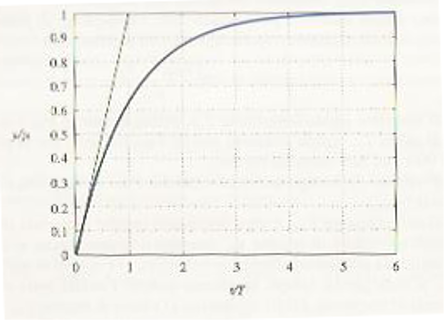
\includegraphics[scale=0.5]{./figures/rispscal1.png}
\caption{Risposta al gradino del sistema \ref{eq:firstordfdt}}\label{fig:risp1}
\end{center}
\end{figure} 
Nota: ad una diminuzione di $T$, cio\`e ad uno spostamento verso
sinistra del polo, corrisponde una diminuzione del tempo di salita,
del tempo di ritardo e del tempo di assestamento.

\section{Sistemi del $II^{\circ}$ ordine}
\subsection{Sistemi con solo poli reali}
\subsubsection{Caso 1: poli distinti}
\begin{equation}\label{eq:secordfdt_c1}
  G(s) = \dfrac{\mu}{(1+sT_1)(1+sT_2)} \qquad, \qquad T_1>T_2
\end{equation}
Appicando la teoria dei fratti semplici, abbiamo che la risposta al
gradino \`e:
\[
  \dfrac{A}{s} + \dfrac{B}{(1 + sT_1)} + \dfrac{C}{(1 + sT_2)} =
  \dfrac{\mu}{(1 + sT_1)(1 + sT_2)s}
\]
Moltiplichiamo ambo i membri per $s$ e facciamo tendere $s$ a zero:
\[
  \dfrac{\mu \xout{s}}{(1 + \xout{sT_1})(1 + \xout{sT_2})\xout{s}} = A
  + 0 + 0
\]
\[
  A = \mu
\]
Stesso discorso per $B$ e $C$. Avremo in questo modo:
\[
  Y(s) = \dfrac{\mu}{s} - \mu \dfrac{\frac{T_1^2}{(T_1 - T_2)}}{(1 + sT_1)} -
  \mu \dfrac{\frac{T_2^2}{(T_1 - T_2)}}{(1 + sT_2)}
\]
Mettendo in evidenza $\mu$ ed antitrasformando, otteniamo:
\begin{equation}\label{eq:rispgradsec_c1}
  y(t) = \mu \left( 1 - \frac{T_1}{T_1-T_2} e^{-\frac{t}{T_1}} +
  \frac{T_2}{T_1-T_2} e^{-\frac{t}{T_2}} \right) \qquad, \qquad t \ge 0
\end{equation}

\begin{figure}[!h]
  \begin{center}
    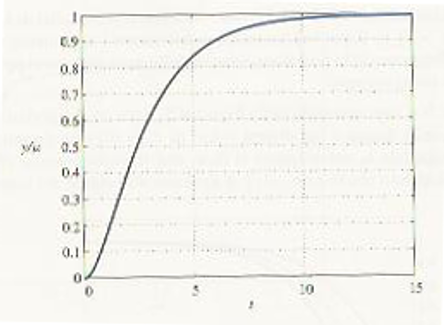
\includegraphics[scale=0.5]{./figures/rispscal2.png}
    \caption{Risposta al gradino del sistema \ref{eq:secordfdt_c1}}
    \label{fig:risp2}
  \end{center}
\end{figure} 

Alcune considerazioni conclusive:
\begin{itemize}
\item La risposta $y(t)$ ci mostra la presenza di due transitori;
\item La posizione del polo influenza la costante di tempo e, di
  conseguenza, la prontezza del sistema: pi\`u il polo \`e vicino allo
  zero pi\`u la costante di tempo \`e grande e pi\`u il sistema evolve
  lentamente;
\item La risposta non presenta sovraelongazione.
\end{itemize}

\subsubsection{Caso 2: poli coincidenti $(T_1 = T_2 = T)$}
\begin{equation}\label{eq:secordfdt_c2}
  G(s) = \dfrac{\mu}{(1 + sT)^2}
\end{equation}
La risposta al gradino della \ref{eq:secordfdt_c2} \`e:
\begin{equation}\label{eq:rispgradsec_c2}
  y(t) = \mu \left( 1 - e^{-\frac{t}{T}} -
  \dfrac{t}{T}e^{-\frac{t}{T}} \right)\qquad, \qquad t\ge 0
\end{equation}
I parametri caratteristici sono:
\begin{itemize}
\item $y_{\infty} = \mu$
\item $T_s \simeq 3.36T$
\item $T_r \simeq 1.68T$
\item $T_{a5} \simeq 4.74T$
\item $T_{a1} \simeq 6.64T$
\end{itemize}

\subsection{Sistemi con poli reali e uno zero}
\begin{equation}\label{eq:secordfdt_cc1}
  G(s)= \dfrac{\mu(1 + \tau s)}{(1 + sT_1)(1 + sT_2)}\qquad, \qquad
  T_1\neq\tau, T_2\neq \tau 
\end{equation}
Applicando, come di consueto la teoria dei fratti semplici, la
risposta al gradino della \ref{eq:secordfdt_cc1} \`e: 
\begin{equation}\label{eq:rispgradsec_cc1}
  y(t) = \mu \left( 1 - \dfrac{T_1-\tau}{T_1 - T_2}e^{-\frac{t}{T_1}} + 
  \dfrac{T_2 - \tau}{T_1 - T_2}e^{-\frac{t}{T_2}}\right) \qquad,
  \qquad t\ge0 
\end{equation}
In funzione della posizione dello zero rispetto ai poli, supposto $T_1
> T_2 > 0$, si distinguono i seguenti casi:

\subsubsection{I caso: $\tau < 0$}
La risposta, come mostrato in figura \ref{fig:risp3}, presenta una
\emph{sottoelongazione} iniziale, o {\em
  risposta inversa}\index{Risposta inversa}, che \`e tanto pi\`u
pronunciata quanto pi\`u lo zero $- \dfrac{1}{\tau}$ si avvicina
all'origine del piano complesso. 
\begin{figure}[!h]
\begin{center}
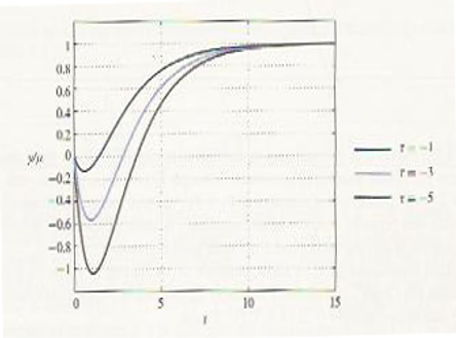
\includegraphics[scale=0.5]{./figures/rispscal3.png}
\caption{Risposta al gradino del sistema \ref{eq:secordfdt_cc1} con
  $\tau < 0$} \label{fig:risp3}
\end{center}
\end{figure}
Ricordiamo che la sottoelongazione\index{Sottoelongazione} $\sigma$
\`e definita come:
\begin{equation}
  \sigma  = \left . \frac{{\bar y - y_{\min }}}{{\bar y}} \right|
\end{equation}
dove $y_{\min }$ \`e il minimo valore assunto dall'uscita del sistema
e $\bar{y}$ \`e l'uscita all'equilibrio.

\subsubsection{II caso: $\tau>T_1>T_2$}
In questo caso (figura \ref{fig:risp4}), la risposta presenta una
\emph{sovraelongazione} tanto pi\`u evidente quanto pi\`u lo zero negativo
\`e vicino all'origine del piano complesso, rispetto alla posizione dei
poli. Per i sistemi di ordine elevato la presenza di una
sovraelongazione (da non confondere con andamenti oscillanti) nella
risposta al gradino, indica la presenza di uno zero reale negativo e
minore in modulo ai poli.
\begin{figure}[!h]
  \begin{center}
    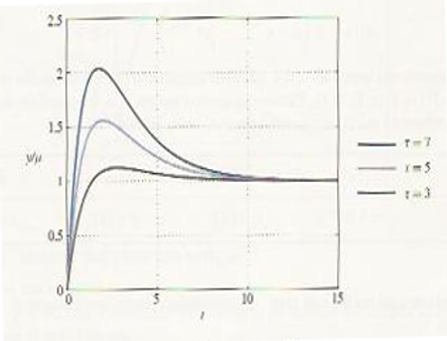
\includegraphics[scale=0.5]{./figures/rispscal4.png}
    \caption{Risposta al gradino del sistema \ref{eq:secordfdt_cc1} con $\tau>0$}\label{fig:risp4}
  \end{center}
\end{figure} 
Ricordiamo che la sovraelongazione\index{Sovraelongazione} $\sigma$
\`e definita come:
\begin{equation}
  \sigma  = \left . \frac{{y_{\max } - \bar y}}{{\bar y}} \right|
\end{equation}
dove $y_{\max }$ \`e il massimo valore assunto dall'uscita del sistema
e $\bar{y}$ \`e l'uscita all'equilibrio.

\subsubsection{III caso: $\tau \simeq T_1\gg T_2$}
Con tali valori di $\tau$ e $T_1$, $T_2$, si pu\`o facilmente verificare
che la \ref{eq:rispgradsec_cc1} diventa approssimativamente:
\begin{equation}\label{eq:2ndOrdineCaso3}
  y(t)\simeq \mu (1 - e^{-\frac{t}{T_2}})\qquad , \qquad t\geq0
\end{equation}
aprossimabile, quindi, ad un sistema del primo ordine. Dalla figura
\ref{fig:risp5} si evince che la coppia polo-zero 
genera comunque un transitorio di piccola entit\`a, il quale fa andare
lentamente $y$ verso $y_\infty$. 
\begin{figure}[!h]\label{fig:risp5}
  \begin{center}
    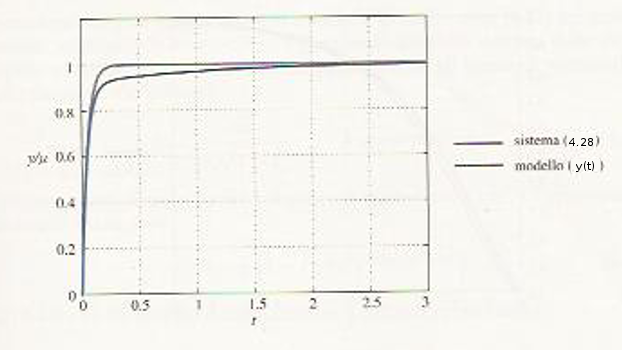
\includegraphics[scale=0.5]{./figures/rispscal5.png}
    \caption{Risposta al gradino del sistema \ref{eq:secordfdt_cc1} con
      $\tau=0.92$}
  \end{center}
\end{figure} 
La \ref{fig:risp5} mostra come l'assenza di un polo nella \ref{eq:2ndOrdineCaso3},
cancellato grazie allo zero, velocizzi il sistema: i poli rallentano,
quindi meno poli portano ad un sistema pi\`u rapido nel raggiungere il
regime. 

\subsubsection{IV caso: $T_1 > \tau > T_2$}
La presenza di uno zero, tende a velocizzare la risposta di un
sistema. In figura \ref{fig:risp6} \`e riportato il caso in cui $T_1 =
2$ e $T_2 = 1$ con valori di $\tau = 0$ e $1.5$ . Con ragionamenti
analoghi al caso III, avendo posto $\tau \simeq T_2$ si ha che la
\ref{eq:rispgradsec_cc1} diventa
\begin{displaymath}
  y(t)\simeq \mu (1-e^{-\frac{t}{T_1}})\qquad , \qquad t\geq0
\end{displaymath}
\begin{figure}[!h]
  \begin{center}
    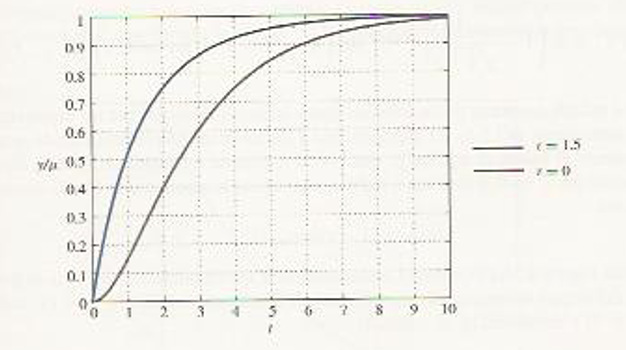
\includegraphics[scale=0.5]{./figures/rispscal6.png}
    \caption{Risposta al gradino del sistema \ref{eq:secordfdt_cc1} con
      due diversi valori di $\tau$}\label{fig:risp6}
  \end{center}
\end{figure}

\subsubsection{V caso: $T_1 > T_2 > \tau > 0$}
Per uno zero che si allontana dall'origine del piano complesso (ovvero
per $\tau$ che diminuisce), la risposta della \ref{eq:rispgradsec_cc1}
tende a diventare come la \ref{eq:rispgradsec_c1}, come mostrato in
figura \ref{fig:risp7}: per uno zero sempre pi\`u lontano dall'origine
del piano complesso, la risposta al gradino di un sistema con poli
reali ed uno zero approssima la risposta di un sistema con solo poli
reali. 
\begin{figure}[!h]
\begin{center}
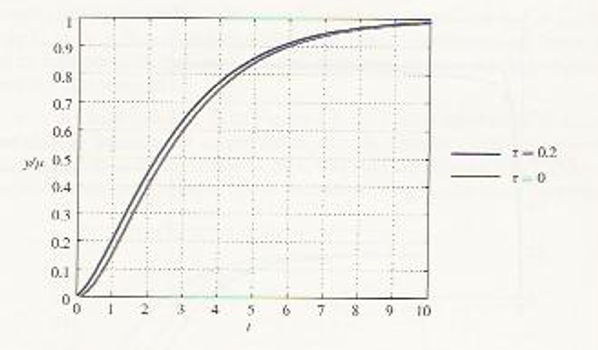
\includegraphics[scale=0.5]{./figures/rispscal7.png}
\caption{Risposta al gradino del sistema \ref{eq:secordfdt_cc1} del
  \emph{caso V}}\label{fig:risp7} 
\end{center}
\end{figure} 

\subsection{Sistemi con poli complessi e coniugati}
La funzione di trasferimento di un sistema avente poli complessi
coniugati \`e:
\begin{equation}\label{eq:fdtcomplex}
  G(s) = \dfrac{\mu \omega^2_n}{s^2 + 2 \xi \omega_n s + \omega^2_n}
\end{equation}
con la pulsazione naturale $\omega_n > 0$ e lo smorzamento dei poli
$\xi$, $|\xi| < 1$. Applicando lo sviluppo in serie di Heaviside, la
risposta al gradino del sistema \ref{eq:fdtcomplex} risulta: 
\begin{equation}\label{eq:rispfdtcomplex}
  y(t) = \mu \left ( 1-\frac{1}{\sqrt{1-\xi^2}}e^{-\xi \omega_n t}\sin
  \left ( \omega_n t\sqrt{1-\xi^2} + \arccos(\xi) \right) \right)
\end{equation}
con $t \geq 0$. Abbiamo quindi un termine esponenziale che moltiplica un
termine sinusoidale, come mostrato in figura \ref{fig:risp8}.
\begin{figure}[!h]
  \begin{center}
    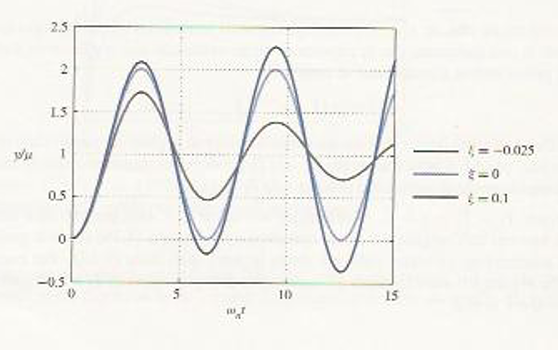
\includegraphics[scale=0.5]{./figures/rispscal8.png}
    \caption{Risposta al gradino del sistema \ref{eq:fdtcomplex}}
    \label{fig:risp8}
  \end{center}
\end{figure} 
In particolare
\begin{itemize}
\item per uno smorzamento $\xi > 0$ (figura \ref{fig:risp9}), il
  sistema \`e ASINTOTICAMENTE STABILE. L'esponenziale \`e decrescente e
  la risposta tende asintoticamente a $\mu$; 
\item per $\xi < 0$ l'esponenziale \`e positivo, il sistema \`e
  INSTABILE e l'uscita \`e divergente; 
\item per $\xi = 0$ l'esponenziale vale $1$, il sistema \`e STABILE,
  ma non asintoticamente e la \ref{eq:rispfdtcomplex} diventa
  \[
    y(t) = \mu(1-\cos(\omega_n t))\qquad , \qquad t\geq0
  \]
\end{itemize}

\begin{figure}[!h]
  \begin{center}
    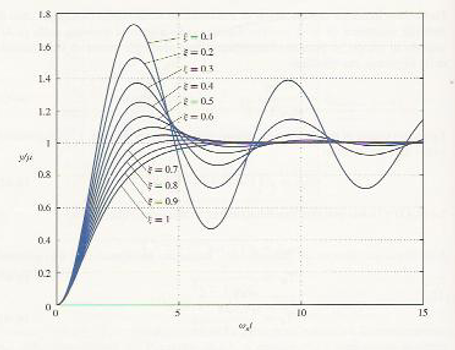
\includegraphics[scale=0.5]{./figures/rispscal9.png}
    \caption{Risposta al gradino del sistema \ref{eq:fdtcomplex} per
      diversi valori di $\xi>0$}\label{fig:risp9}
  \end{center}
\end{figure} 

I parametri caratteristici del sistema con poli complessi e coniugati
sono riassunti nella tabella \ref{tab:tabfdtcomplexparms}:
\begin{table}[!hbp]
  \begin{center}
    \begin{tabular}{|c|c|c|c|c|}
      \hline
      $y_\infty$ & $S\%$ & $T_M$ & $T_P$ & stima di $T_{a\varepsilon}$\\
      \hline
      $\mu$ & $100e^{-\xi \pi / \sqrt1-\xi^2}$ & $\dfrac{\pi}{\omega_n
        \sqrt{1-\xi^2}}$ & $\dfrac{2\pi}{\omega_n \sqrt{1-\xi^2}}$ &
      $-\dfrac{1}{\xi \omega_n}\ln0.01\varepsilon$\\
      \hline
    \end{tabular}
  \end{center}
  \caption{Parametri del sistema \ref{eq:fdtcomplex}}
  \label{tab:tabfdtcomplexparms}
\end{table}

\begin{figure}[!h]
  \begin{center}
    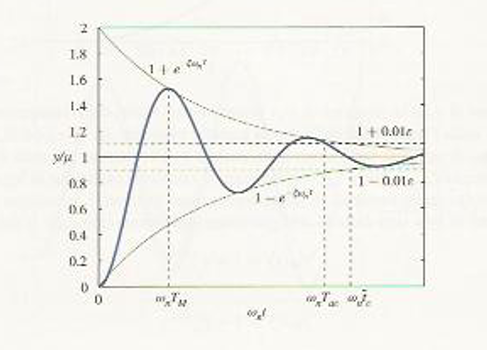
\includegraphics[scale=0.5]{./figures/rispscalX.png}
    \caption{Risposta al gradino del sistema \ref{eq:fdtcomplex} e
      parametri caratteristici}\label{fig:rispX}
  \end{center}
\end{figure} 

% SCHEMI A BLOCCHI - CAPITOLO 5 DEL BOLZERN
\chapter{Interconnessione di sistemi e schemi a blocchi}
I sistemi possono essere collegati in serie, parallelo o in retroazione.

\section{Sistemi in serie}
Abbiamo due sistemi descritti dalle equazioni:
\begin{eqnarray}
  Y_a(s) = G_a(s)U_a(s)\\
  Y_b(s) = G_b(s)U_b(s)
\end{eqnarray}
Essi si dicono connessi in serie (o cascata) quando l'uscita del primo
diventa l'ingresso del secondo: $y_a = u_b$. Quindi, con $u(t) = u_a(t)$
e $y(t) = y_b(t)$, si ricava che 
\begin{equation}
  Y(s) = G_b(s)Y_a(s) = G_b(s)G_a(s)U(s)
\end{equation}
e la funzione di trasferimento diventa
\begin{equation}
  G(s) = \dfrac{Y(s)}{U(s)} = G_a(s)G_b(s)
\end{equation}
ovvero, \emph{la funzione di trasferimento totale di un sistema
  composto dalla serie di due sottosistemi \`e pari al prodotto delle
  singole funzioni di trasferimento}.
\begin{figure}[!hbp]
  \begin{center}
    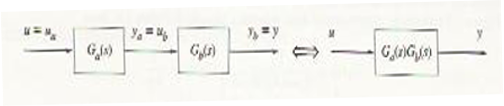
\includegraphics[scale=0.5]{./figures/serie.png}
    \caption{Sistemi connessi in serie}\label{fig:syserie}
  \end{center}
\end{figure}

\section{Sistemi in parallelo}
Due sistemi si dicono connessi in parallelo se hanno lo stesso
ingresso e le loro uscite si sommano, per generare l'uscita del
sistema complessivo. Formalizzando si ha:
\begin{equation}
  Y(s) = Y_a(s) + Y_b(s) = G_a(s)U_a(s) + G_b(s)U_b(s) = (G_a(s) + G_b(s))U(s)
\end{equation}
quindi la funzione di trasferimento \`e:
\begin{equation}
  G(s) = \dfrac{Y(s)}{U(s)} = G_a(s) + G_b(s)
\end{equation}
ovvero \emph{la funzione di trasferimento complessiva di un sistema
  composto dal parallelo di due sottosistemi \`e pari alla somma
  delle singole funzioni di trasferimento}.
\begin{figure}[!hbp]
  \begin{center}
    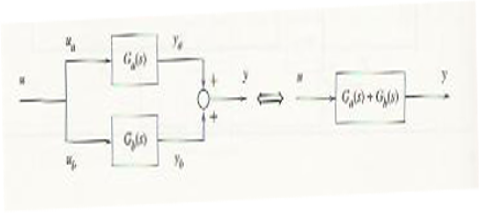
\includegraphics[scale=0.5]{./figures/parallelo.png}
    \caption{Sistemi connessi in parallelo}\label{fig:sysparal}
  \end{center}
\end{figure} 

\section{Sistemi in retroazione}
\begin{figure}[!h]
  \begin{center}
    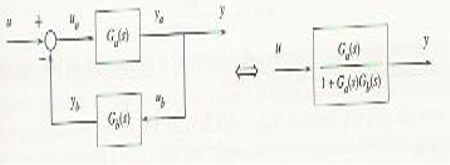
\includegraphics[scale=0.5]{./figures/feedbackneg.png}
    \caption{Sistemi con feedback negativo}\label{fig:sysnegfed}
  \end{center}
\end{figure}
\begin{figure}[!h]
  \begin{center}
    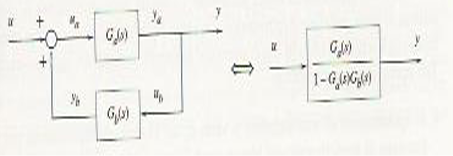
\includegraphics[scale=0.5]{./figures/feedbackpos.png}
    \caption{Sistemi con feedback positivo}\label{fig:sysposfed}
  \end{center}
\end{figure} 
Nelle figure \ref{fig:sysposfed} e \ref{fig:sysnegfed} sono mostrati
dei sistemi aventi due sottosistemi collegati in retroazione\index{Retroazione} o
feedback\index{Feedback} o in anello chiuso\index{Anello chiuso}.
Si ricava che:
\begin{equation}
  Y(s) = G_a(s)(U(s) - Y_b(s)) = G_a(s)(U(s) - G_b(s)Y(s))
\end{equation}
pertanto la funzione di trasferimento complessiva per la
\emph{retroazione negativa} \`e:
\begin{equation}
  G(s) = \dfrac{Y(s)}{U(s)} = \dfrac{G_a(s)}{1 + G_a(s)G_b(s)}
\end{equation}
mentre quella in \emph{retroazione positiva} \`e
\begin{equation}
  G(s)=\dfrac{Y(s)}{U(s)} = \dfrac{G_a(s)}{1 - G_a(s)G_b(s)}
\end{equation}
ovvero \emph{la funzione di trasferimento di un sistema avente due
  sottosistemi retroazionati negativamente (o positivamente) \`e pari al
  rapporto tra la funzione di trasferimento del sottosistema che
  appare lungo la linea di andata tra $u$ e $y$ e la somma (o
  differenza) tra $1$ e il prodotto delle singole funzione di
  trasferimento, detto in questo caso funzione di trasferimento
  d'anello $L(s)$} 
\begin{equation}
  L(s)=G_a(s)G_b(s)
\end{equation}

\subsection{Semplificazione di schemi a blocchi}
Quando lo schema a blocchi  di un sistema, presenta un numero
abbastanza elevato di ``sotto-blocchi'' (ovvero funzioni di
trasferimento), \`e necessario effettuare delle operazioni di riduzione
dello stesso in modo da semplificare l'analisi ed i calcoli. L'operazione
di riduzione e lo spostamento dei blocchi sono rese possibili grazie
alla propriet\`a di \emph{linearit\`a }. Si possono applicare, a tale
scopo, semplici manipolazioni utilizzando le regole di serie,
parallelo e retroazione. Si possono, poi, applicare le seguenti
ulteriori regole: 
\begin{itemize}
\item Per spostare una variabile ``a valle'' di un blocco, \`e necessario
  moltiplicarla per la funzione di trasferimento del blocco;
\item Per spostare una variabile ``a monte'' di un blocco, \`e necessario
  dividerla per la funzione di trasferimento del blocco;
\item Per spostare un blocco ``a monte'' di un nodo sommatore, bisogna
  moltiplicare la funzione di trasferimento del blocco per tutte le
  altre variabili entranti nel nodo;
\item Per spostare un blocco ``a valle'' di un nodo sommatore, bisogna
  dividere la funzione di trasferimento del blocco per tutte le altre
  variabili entranti nel nodo.
\end{itemize}
Per quel che riguarda la stabilit\`a dei sistemi in serie, parallelo e
in retroazione possiamo affermare che:
\begin{itemize}
\item La connessione in serie di sottosistemi asintoticamente stabili
  genera {\em sempre} un sistema asintoticamente stabile;
\item La presenza di un sottosistema non asintoticamente stabile in un
  collegamento in serie rende il sistema complessivo anch'esso non
  asintoticamente stabile;
\item La connessione in parallelo di sottosistemi asintoticamente
  stabili genera {\em sempre} un sistema asintoticamente stabile;
\item La presenza di un sottosistema non asintoticamente stabile in un
  collegamento in parallelo rende non asintoticamente stabile il
  sistema complessivo;
\item La connessione in retroazione di sistemi asintoticamente stabili
  pu\`o generare un sistema {\em non} asintoticamente stabile;
\item Un sistema retroazionato pu\`o essere asintoticamente stabile
  anche se alcuni dei sottosistemi non sono asintoticamente stabili;
\end{itemize}
Le figure presenti in figura \ref{fig:blockex} aiutano a capire le
possibili riduzioni che si possono effettuare sugli schemi a blocchi: 
\begin{figure}[!hbp]
  \begin{center}
    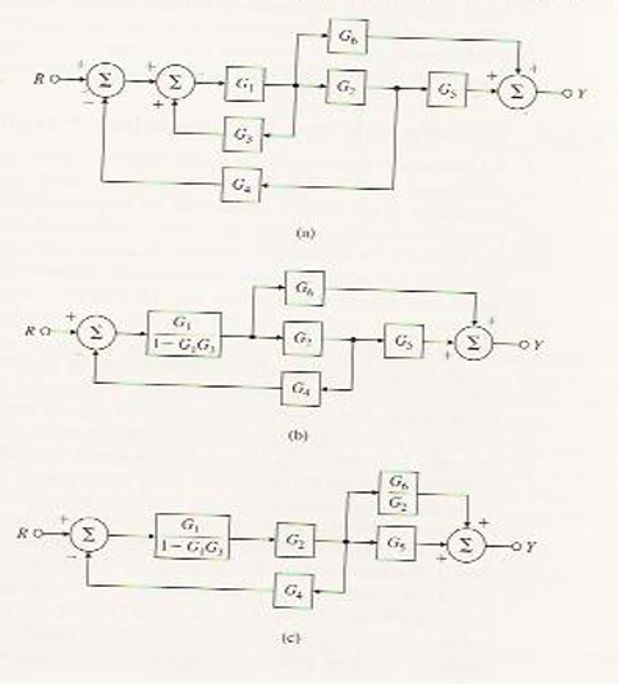
\includegraphics[scale=0.5]{./figures/block_example.png}
    \caption{Esempio di riduzione di schemi a blocchi}
    \label{fig:blockex}
  \end{center}
\end{figure} 

\chapter{Modelli matematici}
Il primo passo per la costruzione di un sistema di controllo \`e lo
sviluppo di una descrizione matematica del processo da
controllare. L'insieme delle equazioni differenziali che descrivono il
comportamento dinamico del processo \`e detto {\bf modello}.

\section{Sistemi Meccanici}
\begin{figure}[!b]
\centering
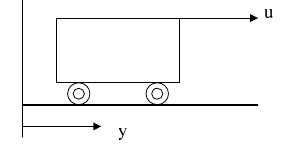
\includegraphics[width=0.5\textwidth]{./images/carrello.png}
\caption{Carrellino\label{fig:carrello}}
\end{figure}
\subsection{Carrello}\label{carrello}
Il carrello di figura \ref{fig:carrello} \`e modellabile come una massa $m$ che si muove spinta da
un ingresso $u$ fino ad un punto $y$. L'equazione del moto del
sistema, stando alla Legge di Newton (\ref{leggedinewton}), 
\`e quindi:
\begin{equation}
  F = m \cdot a \Rightarrow u = m \cdot \ddot{y}
\end{equation}
Integrando due volte si otttiene:
$$y(t) = y(0) + \dot{y}(0) + \int_0^t \left ( \int_o^{\theta} u(\tau)d\tau
\right ) d \theta$$
La soluzione dell'equazione differenziale dipende dallo stato iniziale
del carrello. Se ``sostituiamo'' i differenziali con le $s$ otteniamo
la funzione di trasferimento:
$$y = \frac{1}{ms^2} \cdot u$$
Volendo ottenere la rappresentazione in forma di stato poniamo $x_1 =
y$ e $x_2 = \dot{y}$ e riscriviamo il tutto come:
\begin{eqnarray*}
  \left\{ \begin{array}{l}
    \dot{x_1} = x_2\\
    \dot{x_2} = \frac{1}{m} \cdot u\\
    y = x_1
    \end{array}\right .
\end{eqnarray*}
Per i sistemi \`e, inoltre, possibile riscrivere il tutto in forma
matriciale. Il carrello \`e un sistema lineare e quindi:
\begin{eqnarray*}
  \begin{array}{l}
    \dot{x} = 
    \begin{bmatrix}
      0 & 1\\
      0 & 0
    \end{bmatrix}
    x + 
    \begin{bmatrix}
      0\\
      \frac{1}{m}
    \end{bmatrix}u
    \\
    y = \begin{bmatrix}1 & 0 \end{bmatrix}x
    \end{array}
\end{eqnarray*}
Nota: possiamo considerare il sistema come una serie di due
``blocchetti''. Un primo che ne specifica i comportamenti dinamici,
fornendo come risultato lo stato del sistema, ed un secondo blocchetto
che specifica il comportamento statico, che riceve in ingresso lo
stato e fornisce l'uscita totale del sistema.

\begin{figure}[!b]
\centering
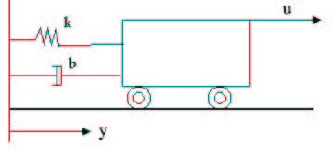
\includegraphics[width=0.5\textwidth]{./images/massa-molla-smorzatore.png}
\caption{Massa-molla-smorzatore\label{fig:massa-molla-smorzatore}}
\end{figure}

\subsubsection{Legge di Newton}\label{leggedinewton}
Per ottenere un modello matematico per qualsiasi sistema meccanico \`e
fondamentale la Legge di Newton, che per il moto traslatorio \`e:
\begin{equation}
  F = ma = m \cdot \dot{v} = m \cdot \ddot{p}
\end{equation}
dove $v$ e $p$ sono rispettivamente ``velocit\`a'' e ``posizione'',
$F$ \`e la somma vettoriale delle forze applicate al sistema (misurata
in Newton: una forza di 1 newton imporr\`a una accelerazione di 1
$\dfrac{m}{s^2}$ ad una massa di un kg), $m$ \`e la massa
(kg) e $a$ \`e l'accelerazione inerziale $\left(\frac{m}{s^2}\right)$.
Il metodo per risolvere questo tipo di problema utilizzando la Legge
di Newton \`e definito dal seguente procedimento:

\begin{itemize}
  \item assegnare delle variabili necessarie e sufficienti per
    descrivere una posizione arbitraria dell'oggetto rispetto ad un
    sistema inerziale
  \item disegnare lo schema di ogni componente indicando le forze
    agenti
  \item applicare la Legge di Newton
  \item combinare le equazioni per eliminare le forze interne: il
    numero delle equazioni indipendenti deve essere uguale al numero
    delle incognite
  \item valutare accuratamente la scelta delle coordinate
\end{itemize}

\subsection{Massa-molla-attrito}
In figura \ref{fig:massa-molla-smorzatore} abbiamo le seguenti variabili:
$k$ \`e il coeffiente elastico della molla, $b$ \`e il coeffiente di
attrito dello smorzatore, $u$ \`e la forza applicata, $y$ \`e lo
spostamento. Dalla formula di Newton (\ref{leggedinewton}) si arriva rapidamente
all'equazione del moto del sistema:
\begin{equation}\label{massa-molla-attrito}
u -ky -b\dot{y} = m \ddot{y}
\end{equation}
Notiamo come l'attrito sia proporzionale alla posizione $y$, mentre lo
smorzamento sia proporzionale alla velocit\`a $\dot{y}$. Sfruttando le
``sostituzioni di Laplace'' ($\dot{y} \rightarrow sy$, $\ddot{y}
\rightarrow s^2y$), possiamo riscrivere la funzione di trasferimento come:
$$m s^2 y + b s y + k y = u \Rightarrow y = \left ( \frac{1}{m s^2 +
  bs + k} \right )u$$
La rappresentazione di stato permette di scrivere l'equazione della
funzione di trasferimento come sistema di equazioni del primo
ordine. Posti $x_1 = y$ e $x_2 = \dot{y}$ si ha:
\begin{eqnarray*}
  \left\{ \begin{array}{l}
    \dot{x}_1 = x_2\\
    \dot{x}_2 = -\left(\dfrac{k}{m}\right)x_1 - \left(\dfrac{b}{m}\right)x_2 + \dfrac{u}{m}\\
    y = x_1
    \end{array}\right .
\end{eqnarray*}
La rappresentazione di stato in forma matriciale:
\begin{eqnarray*}
  \left\{ \begin{array}{lr}
    \dot{x} = \begin{bmatrix}0 & 1\\-\frac{k}{m} &
      -\frac{b}{m}\end{bmatrix}x
    + \begin{bmatrix}0\\ \frac{1}{m}\end{bmatrix}u & \textrm{Come
      l'ingresso modifica lo stato}\\
    y = \begin{bmatrix}1 & 0\end{bmatrix}x & \textrm{Come lo stato
        influisce sull'uscita}
    \end{array}\right .
\end{eqnarray*}
\subsubsection{Stato e uscita di equilibrio}
Supponiamo un ingresso $u = \overline{u}$ costante. \`E sufficiente
ora porre le derivate dello stato uguali a zero:
\begin{eqnarray*}
  \left\{ \begin{array}{l}
    \overline{x_2} = 0\\
    \overline{u} - k \overline{x_1} = 0
    \end{array}\right .
  \Rightarrow
  \left\{ \begin{array}{l}
    \overline{x_2} = 0\\
    \overline{x_1} = \dfrac{\overline{u}}{k}
  \end{array}\right .
  \Rightarrow
  \overline{y} = \dfrac{1}{k} \overline{u} \;\; \textrm{che \`e l'uscita di equilibrio}
\end{eqnarray*}
Il valore $\frac{1}{k} = \frac{\overline{y}}{\overline{u}}$ \`e detto
{\em guadagno statico}\index{Guadagno statico} e per ottenerlo \`e
sufficiente porre $s = 0$ nella funzione di trasferimento. Non sempre
un sistema presenta un guadagno statico. Un sistema senza punti di
equilibrio \`e un sistema senza guadagno statico:
$$\textrm{Punto di equilibrio} \Leftrightarrow \textrm{Guadagno statico}$$

\subsection{Sospensioni}
\begin{figure}[!b]
\centering
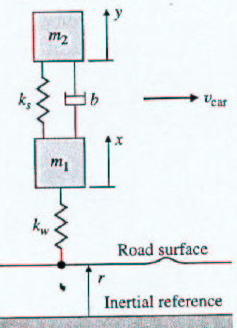
\includegraphics[width=0.4\textwidth]{./images/sospensioni.png}
\caption{Sospensioni\label{fig:sospensioni}}
\end{figure}
Assumiamo il moto della massa dell'automobile su una ruota come
monodimensionale, cio\`e solo verticale. $k_s$ \`e il coeffiente di
elasticit\`a delle sospensioni, $b$ \`e il coeffiente di smorzamento
delle sospensioni, $k_w$ \`e il coeffiente di elasticit\`a del
pneumatico, $m_1$ \`e la massa della ruota, $m_2$ \`e la massa
dell'auto, $u$ \`e la superficie stradale. Il modello tralascia
volutamente la forza di gravit\`a. Lo smorzamento introdotto dalla
sospensione \`e considerato proporzionale alla velocit\`a di
variazione dello spostamento relativo tra le due masse, cio\`e a
$b(\dot{y} - \dot{x})$. Per comodit\`a consideriamo un modello ad
elementi separati, separando le due masse ed analizzandole singolarmente.


Dal punto di vista della della ruota ($m_1$), si hanno tre contributi:
il contributo della molla $k_w$, che rappresenta l'elasticit\`a del
pneumatico, \`e diretto verso il suolo; il contributo della molla
$k_s$ e dello smorzatore $b$ che rappresentano la sospensione e sono
diretti verso l'automobile.

Dal punto di vista dell'automobile ($m_2$) abbiamo solo i contributi
della molla $k_s$ e dello smorzatore $b$, entrambi rivolti verso la ruota.
Il modello complessivo \`e:
\begin{equation}\label{sospensionem1}
  k_s(y-x) + b(\dot{y} - \dot{x}) - k_w(x-r) = m_1\ddot{x}
\end{equation}

\begin{equation}\label{sospensionem2}
  -k_s(y-x) -b(\dot{y} - \dot{x}) = m_2 \ddot{y}
\end{equation}

Cerchiamo la funzione di trasferimento del sistema considerando come
ingresso $r$ e come uscita la sola $y$:
$$G(s) = \frac{Y(s)}{R(s)}$$
Dalla \ref{sospensionem1} otteniamo:
\begin{eqnarray*}
  \begin{array}{l}
    k_s(y-x) + bs(y-x) - k_w(x-r) = m_1s^2x\\
    k_sy - k_sx + bsy - bsx - k_wx + k_wr - m_1s^2x = 0\\
    k_wr = (k_s + bs + k_w + m_1s^2)x - (k_s +bs)y
  \end{array}
\end{eqnarray*}
Dalla \ref{sospensionem2} otteniamo:
\begin{eqnarray*}
  \begin{array}{l}
    -k_s(y-x) -  bs(\dot{y} - \dot{x}) = m_2s^2y\\
    (m_2 s^2 +k_s +bs)y - (k_s + bs)x = 0
  \end{array}
\end{eqnarray*}
\begin{eqnarray*}
  \left\{ \begin{array}{l}
    k_wr = (k_s + bs + k_w + m_1s^2)x - (k_s +bs)y\\
    (m_2 s^2 +k_s +bs)y - (k_s + bs)x = 0
    \end{array}\right .
\end{eqnarray*}
La funzione di trasferimento che si ottiene \`e:
$$\dfrac{Y(s)}{R(s)} = \dfrac{\dfrac{k_wb}{m_1m_2} \left( s +
  \dfrac{k_s}{b}\right)}{s^4 + \left( \dfrac{b}{m_1} +
  \dfrac{b}{m_2}\right)s^3 + \left( \dfrac{k_s}{m_1} +
  \dfrac{k_s}{m_2} + \dfrac{k_w}{m_1}\right)s^2 + \left( \dfrac{k_w
  b}{m_1 m_2}\right)s + \dfrac{k_w k_s}{m_1 m_2}}$$

Valutiamo ora la rappresentazione in termini di variabili di stato,
ponendo $x_1 = x$, $x_2 = \dot{x}$, $x_3 = y$, $x_4 = \dot{y}$:
\begin{eqnarray*}
  \left\{ \begin{array}{l}
    \dot{x_1} = x_2\\
    \dot{x_2} = \frac{k_s}{m_1}(x_3 - x_1) + \frac{b}{m_1}(x_4 - x_2)
    - \frac{k_w}{m_1}(x_1 - r)\\
    \dot{x_3} = x_4\\
    \dot{x_4} = \frac{k_s}{m_2}(x_3 - x_1) + \frac{b}{m_2}(x_4 -
    x_2)\\
    x = x_1\\
    Y = x_3
    \end{array}\right .
\end{eqnarray*}
Mentre in termini matriciali, posto:
\[
  x = 
  \begin{bmatrix}
    x_1\\
    x_2\\
    x_3\\
    x_4
  \end{bmatrix}
\]
possiamo scrivere:
\[
  \dot{x} = 
  \begin{bmatrix}
    0 & 1 & 0 & 0\\
    -\frac{k_s - k_w}{m_1} & -\frac{b}{m_1} & \frac{k_s}{m_1} &
    \frac{b}{m_1}\\
    0 & 0 & 0 & 1\\
    -\frac{k_s}{m_2} & \frac{b}{m_2} & -\frac{k_s}{m_2} &
    -\frac{b}{m_2}
  \end{bmatrix}x +
  \begin{bmatrix}
    0\\
    \frac{k_w}{m_1}\\
    0\\
    0
  \end{bmatrix}r
\]

\[
  \begin{bmatrix}
    y\\x
  \end{bmatrix} = 
  \begin{bmatrix}
    0 & 0 & 1 & 0\\
    1 & 0 & 0 & 0
  \end{bmatrix}x
\]
All'equilibrio le derivate sono nulle e si trova che lo stato di
equilibrio del sistema \`e:

\[
  \left\{
  \begin{array}{l}
    \overline{x_2} = \overline{x_4} = 0\\
    \overline{x_1} = \overline{x_3} = r
  \end{array} \right .
\]
A corredo del precedente esempio, consigliamo l'esercizio 2.1 di
pagina 78 del Franklin Powell e relativa soluzione presente nel file
\url{http://ur1.ca/9fzq} . Un dato importante che emerge dall'analisi
di questo tipo di sistemi \`e la necessit\`a di valutare singolarmente
le diverse masse e scegliere accuratamente i sistemi di
riferimento. Osservando con attenzione la soluzione dell'esercizio del
Franklin Powell si nota un differente approccio rispetto a quello
mostrato in questo paragrafo. Ad un'analisi piu' approfondita si
noter\`a che le soluzioni sono equivalenti. \`E la scelta dei sistemi
di riferimento che \`e differente.
\subsubsection{Errori di segno}
La principale fonte di errori sono i ``segni''. Una volta ottenute le
equazioni di un sistema stabile non ci resta che controllare i
segni delle varie variabili. Tutti i segni devono essere
concordi. Considerando il predente esempio, tutte le variabili
$\ddot{x}$, $\dot{x}$ ed $x$ hanno segno concorde. Stesso discorso per
le $\ddot{y}$, $\dot{y}$ e $y$.

\subsection{Moto rotatorio}
Per il moto rotatorio la Legge di Newton si modifica nel seguente modo:

\begin{equation}\label{momentodelleforze}
  M = I \alpha
\end{equation}
dove $M$ \`e il {\em momento delle forze}\index{Momento delle forze} applicate al
sistema (misurato in $N \cdot m$ e spesso indicato alternativamente
con $\tau$), $I$ \`e il {\em momento di inerzia}\index{Momento di
  inerzia} del corpo rispetto all'asse di rotazione ($I = mr^2$) ed
$\alpha$ \`e l'{\em accelerazione
  angolare}\index{Accelerazione angolare} (misurata in $\frac{rad}{s^2}$).
% IMMAGINE DI PAGINA 14
Supponiamo di avere una massa $m$ che si muova nello spazio con
velocit\`a $\vec{v}$. Definiamo la {\em quantit\`a di
  moto}\index{Quantit\`a di moto} come:
\begin{equation}
  \vec{p} = m \vec{v}
\end{equation}
e definiamo la forza come variazione della quantit\`a di moto
$\Rightarrow \vec{F} = \dfrac{d\vec{p}}{dt}$.
Si definisce {\em Momento della quantit\`a di moto}\index{Momento
  della quantit\`a di moto} del punto materiale $m$ rispetto ad un
riferimento fissato $O$ il vettore $\vec{e}$:
\begin{equation}
  \vec{e} \equiv \vec{r^{'}} \times \vec{p}
\end{equation}
Supponiamo che su $m$ sia applicata una forza $\vec{F}$; allora
definiamo il {\em Momento delle forza applicate}\index{Momento delle
  forza} al punto materiale $m$ come:
\begin{equation}
  \vec{\tau} = \vec{r^{'}} \times \vec{F}
\end{equation}
Calcoliamo la derivata temporale di $\vec{e}$:
$$\frac{d \vec{e}}{dt} = \frac{d \vec{r^{'}}}{dt} \times \vec{p} +
\vec{r^{'}} \times \frac{d \vec{p}}{dt} = \frac{d \vec{r^{'}}}{dt}
\times \vec{p} = \vec{\tau}$$
Ma \`e anche vero che:
$$\vec{r^{'}} = \vec{r} - \vec{r_0} \Rightarrow \frac{d
  \vec{r^{'}}}{dt} = \frac{d (\vec{r} - \vec{r_0})}{dt} =
\frac{d\vec{r}}{dt} - \frac{d \vec{r^{'}}}{dt} = \vec{v} -
\xout{\vec{v_0}} = \vec{v}$$
$$\Rightarrow \frac{d \vec{e}}{dt} = \xout{\vec{v} \times \vec{p}} +
\vec{\tau} \Rightarrow \frac{d \vec{e}}{dt} = \vec{\tau}$$

% IMMAGINI DI PAGINA 15

Se invece di un punto materiale, consideriamo un insieme di punti
materiali ognuno con una sua massa e velocit\`a e su cui agiscono
delle forze. Detto $i$ il generico punto materiale, supponiamo che
$m_i$ si muova con velocit\`a $v_i$ e che sia sottoposto ad una forza
$\vec{F_i}$. Il momento della quantit\`a di moto del punto $i$ sar\`a
(per ogni $i$):
$$\frac{d \vec{e_i}}{dt} = \vec{\tau_i}$$
Sommiamo tutte le equazioni degli $N$ punti materiali:
$$\sum_{i=1}^{N} \frac{d \vec{e_i}}{dt} = \sum_{i=1}^{N}
\vec{\tau_i}$$
La derivazione \`e indipendente dalla operazione di somma, per cui
``posso invertire e ottengo di nuovo'':
$$\frac{d \vec{L}}{dt} = \vec{\tau}$$
Nota: se il numero di punti \`e infinito, si effettua l'integrale
piuttosto che la somma.

Condideriamo ora un corpo, all'interno di esso consideriamo un
volumetto infinitesimo $dv$ la cui posizione \`e approssimata a quella
di $P$, punto interno a $dv$. Nel volumetto $dv$ c'\`e una massa pari
a: $dm = \mu(p) dv$ dove $\mu(p)$ \`e la densit\`a del corpo. Il
momento della quantit\`a di moto in questo caso \`e:
\begin{equation}\label{L}
\vec{L} = \int_{v} \vec{r_p} \times \mu(p) dv \vec{v}(p)
\end{equation}
Supponiamo che il corpo stia ruotando. Se conosciamo l'asse su cui ruota
possiamo calcolare le componenti del vettore posizione rispetto a
quell'asse. Per semplicit\`a supponiamo che sia l'asse $y$. Ci sono
due componenti, una ortogonale e l'altra parallela all'asse:
$$\vec{v}(p) = \vec{\omega} \times \vec{r_p} = \vec{\omega} \cdot
(\vec{a_p} + \vec{R_p}) = \xout{\vec{\omega} \times \vec{a_p}} +
\vec{\omega} \times \vec{R_p}$$
Nota: dobbiamo considerare solo il contributo ortogonale
all'asse. Sostituiamo $\vec{v}(p)$ nella \ref{L}:
$$\vec{L} = \int_v \vec{r_p} \times \mu(p) (\vec{\omega} \times
\vec{R_p}) dv = \underbrace{\int_v \mu(p) R_p^2 dv}_\text{I} \cdot
\vec{\omega}$$
Ma $I = \int_v \mu(p) R_p^2 dv$ \`e il momento di inerzia e quindi
$\vec{L} = I \vec{omega}$. Derivando, infine, membro a membro
otteniamo:
\begin{equation}
  \frac{d \vec{L}}{dt} = I \frac{d \vec{\omega}}{dt} = \vec{\tau}
  \Rightarrow \vec{\tau} = I \vec{\alpha}
\end{equation}
ottenendo finalmente il principio $F = m \cdot a$ per i moti rotatori
della \ref{momentodelleforze}.
\begin{figure}[!t]
  \centering
  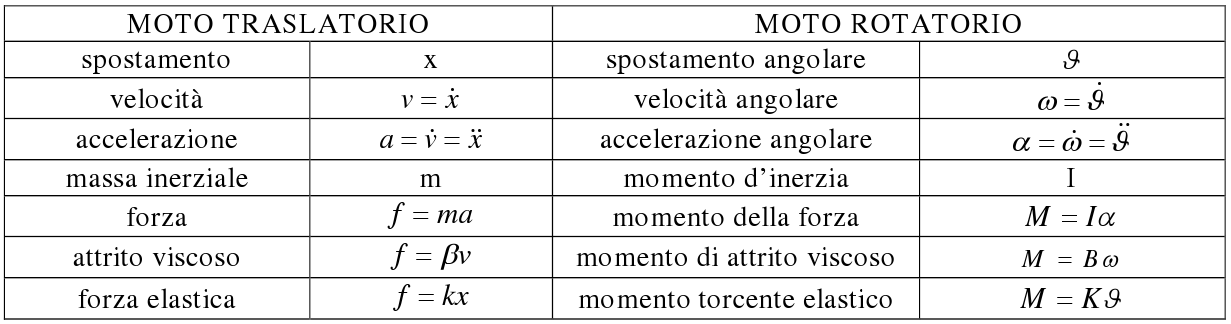
\includegraphics[width=1.0\textwidth]{./images/mototraslatorio-motorotatorio.png}
  \label{fig:mototraslatorio-motorotatorio}
  \caption{Moto traslatorio - Moto rotatorio\label{fig:mototraslatorio-motorotatorio}}
\end{figure}

\subsection{Controllo di un satellite}
\begin{figure}[!h]
  \centering
  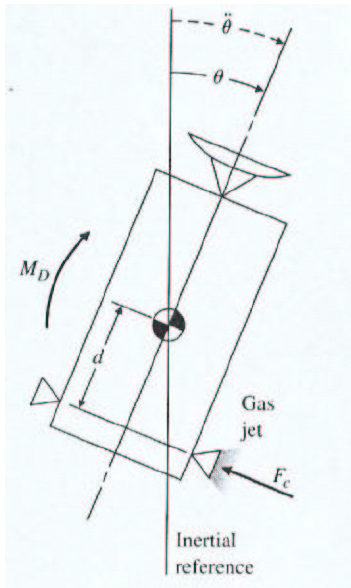
\includegraphics[width=0.3\textwidth]{./images/satellite.png}
  \label{fig:satellite}
  \caption{Schema di controllo di un satellite\label{fig:satellite}}
\end{figure}

Le variabili che considereremo sono la propulsione $F_c$, il momento
delle forze di disturbo $M_D$, la distanza $d$ tra la retta su $F_C$ e
la retta parallela e passante per il centro di massa e infine $y =
\theta$, l'uscita.
La Legge di Newton per il moto
rotatorio\label{leggedinewtonmotorotatorio} \`e:
$$M = I \alpha$$
con $M$ pari alla somma di tutti i momenti esterni, $I$ pari al
momento di inerzia del corpo e $\alpha$ pari al momento angolare.
Applicando la legge sul moto rotatorio e considerando
che sul satellite agisce una forza provocata dalla propulsione che \`e
una coppia di momento $F_c \cdot d$ e un momento $M_D$ dovuto a forze
di disturbo, per lo pi\`u la pressione solare sulle superfici
asimmetriche dei pannelli solari:
$$F_C \cdot d + M_D = I \ddot{\theta}$$
Le ipotesi semplificative sono quindi due: il motore che agisce come
una coppia e il moto in un piano ortogonale all'asse di
rotazione. L'uscita di questo sistema si ottiene per doppia
integrazione della somma della coppie di ingresso. Per questa ragione
questo sistema viene spesso detto {\em doppio
  integratore}\index{Doppio integratore}. La funzione di trasferimento
partendo dall'equazione del moto \`e:

\[
  F_c \cdot M_D = I s^2 \theta \Rightarrow \frac{\theta(s)}{U(s)} =
  \frac{1}{Is^2} \binom{\textrm{2 ingressi}}{\textrm{1 uscita}}
\]
La rappresentazione di stato, posto $x_1 \equiv \theta$ e $x_2 \equiv
\dot{\theta}$ \`e:
\[
  \left\{
  \begin{array}{l}
    \dot{x_1} = x_2\\
    \dot{x_2} = \frac{M_D}{I} + \frac{(F_C \cdot d)}{I}\\
    y = \theta = x_1
  \end{array}\right .
  \Rightarrow
  \begin{array}{l}
    \dot{x} = 
    \begin{bmatrix}
      0 & 1\\
      0 & 0
    \end{bmatrix}x +
    \begin{bmatrix}
      0\\
      \frac{1}{I}
    \end{bmatrix}u\\
    y =
    \begin{bmatrix}
      1 & 0
    \end{bmatrix}x
  \end{array}
\]
Per questo sistema non esiste alcun punto di equilibrio. \'E
deducibile anche dal fatto che manca una qualsiasi forza che si
opponga ad $F_C$.

\subsection{Disco rotante intorno ad un asse con attrico}\label{par:discorotanteattrito}
\begin{figure}[!b]
  \centering
  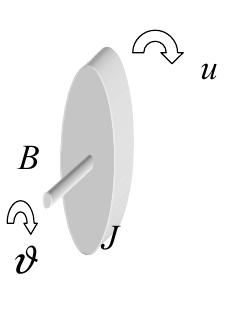
\includegraphics[width=0.2\textwidth]{./images/discorotanteattrito.png}
  \label{fig:discorotanteattrito}
  \caption{Schema di disco rotante con attrito\label{fig:discorotanteattrito}}
\end{figure}
Le variabili del sistema sono: la coppia motrice in ingresso $u$, il
momento inerziale $I$, lo spostamento angolare $\theta$ e il coeffiente
di attrito $B$. L'equazione del moto \`e:
$$u - B \dot{\theta} = I \ddot{\theta} \;\;\;\textrm{con}\;\;\; I =
\frac{1}{2} m_D R^2$$
La rappresentazione di stato \`e:
\[
  \left\{
  \begin{array}{l}
    \dot{x_1} = x_2 = \dot{\theta}\\
    \dot{x_2} = -\frac{B}{I}x_2 + \frac{u}{I}\\
    y = x_1 = \theta
  \end{array}\right .
\]
La funzione di trasferimento \`e:
\[
  \begin{array}{l}
    \ddot{\theta} = -(\frac{B}{I})\dot{\theta} + \frac{u}{y}\\
    s^2 y = -\frac{B}{I} \cdot sy + \frac{u}{I}\\
    s^2 y + \frac{B}{I} sy = \frac{u}{I}\\
    \frac{y}{u}(s^2 + \frac{B}{I}s) = \frac{u}{I} \cdot \frac{1}{u}
  \end{array}
\]
$$G(s) = \frac{1}{I(s^2 + \frac{B}{I}s)} = \frac{1}{s^2 I +sB}$$

\subsection{Disco rotante intorno ad un asse con attrico ed
  elasticit\`a}
\begin{figure}[!b]
  \centering
  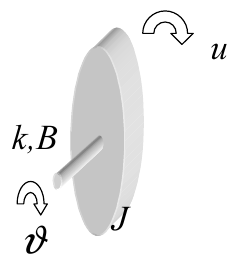
\includegraphics[width=0.2\textwidth]{./images/discorotanteattritoelasticita.png}
  \label{fig:discorotanteattritoelasticita}
  \caption{Schema di disco rotante con attrito ed elasticit\`a\label{fig:discorotanteattritoelasticita}}
\end{figure}
Consideriamo lo stestto esempio. In questo caso, per\`o, \`e presente
anche una certa elasticit\`a dell'asse di rotazione, con $k$ costante
elastica. L'equazione del moto \`e:
$$u - B\dot{\theta} - k \theta = I \ddot{\theta}$$
La funzione di trasferimento \`e:
$$s^2 I \theta = u - s B \theta - k \theta \Rightarrow
\frac{\theta}{u} = \frac{1}{s^2 I + s B  + k}$$
Si nota che l'equilibrio \`e del tutto simile a quella del caso
massa-molla-attrito. Essendo la stessa funzione di trasferimento del
caso massa-molla-attrito (eq. \ref{massa-molla-attrito}) non \`e
necessario procedere con le considerazioni sullo stato, l'equilibrio e
la rappresentazione matriciale.

\subsection{Satellite-Terra}
\begin{figure}[!b]
  \centering
  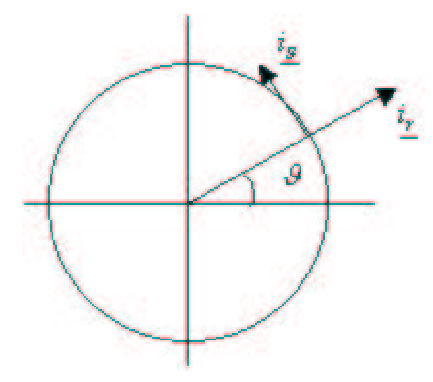
\includegraphics[width=0.5\textwidth]{./images/terrasatellite.png}
  \label{fig:terrasatellite}
  \caption{Schema di un satellite che ruota intorno alla Terra\label{fig:terrasatellite}}
\end{figure}
Le variabili del sistema sono: la Terra $T$, il satellite $S$,
il versore della direzione tangenziale $i_{\theta}$, il versore
della direzione radiale $i_r$. Modelliamo le interazioni tra due corpi
quando uno ruota intorno all'altro (Satellite-Terra). Per semplicit\`a
supporremo che il satellite si muova sempre lungo un'orbita circolare,
sempre sullo stesso piano perpendicolare all'asse di rotazione e le
dimensioni di Terra e satellite siano trascurabili. Questo tipo di
problema si risolve bene in coordinate cilindriche dove $i_r$
(direzione radiale) e $i_{\theta}$ (direzione tangenziale) ruotano
anch'essi. Da ricordare, la {\em Legge di gravitazione
  universale}\index{Legge di gravitazione universale}:
$$-k \frac{M_T M_S}{r^2}$$
e le {\em Relazioni di Poisson}\index{Poisson}:
\[
  \left\{
  \begin{array}{l}
    \dfrac{di_r}{dt} = \dot{\theta}i_{\theta}\\
    \dfrac{di_{\theta}}{dt} = - \dot{\theta} i_r
  \end{array}\right .
\]
Detta $P$ la posizione del satellite: $\vec{P} = r i_r$, ricordando
che $\dot{P} = r \dot{\theta} i_{\theta} + \dot{r}i_r$, derivando due
volte si ottiene l'accelerazione del satellite:
$$\ddot{P} = (\ddot{r} - r \dot{\theta}^2)i_r + (r \ddot{\theta} + 2r \dot{\theta})i_{\theta}$$
Le forze agenti sul satellite sono:
$$F = \left( -k \dfrac{M_T M_S}{r^2} + u_1 \right)i_r + u_2
i_{\theta}$$
Le equazioni del moto lungo i versori $i_r$ e $i_{\theta}$:
\[
  M_S (\ddot{r} - r \dot{\theta}^2) = -k \dfrac{M_T M_S}{r^2} + u_1
\]
\[
  M_S (r \ddot{\theta} + 2r \dot{\theta}) = u_2
\]
Il modello in forma di stato prevede $x_1 = r$, $x_2 = \dot{r}$, $x_3
= \theta$ e $x_4 = \dot{\theta}$:
\[
  \left\{
  \begin{array}{l}
    \dot{x}_1 = x_2\\
    \dot{x}_2 = - \dfrac{k M_T}{x_1^2} + x_1 x_4^2 +
    \dfrac{u_1}{M_S}\\
    \dot{x}_3 = x_4\\
    \dot{x}_4 = -2 x_4 + \dfrac{u_2}{x_1}\\
    y_1 = x_1\\
    y_2 = x_3
  \end{array}
  \right .
\]
ANDREBBE INTEGRATO, MA NON RIESCO A TROVARE MATERIALE

\subsection{Pendolo}\label{pendolo}
\begin{figure}[!h]
  \centering
  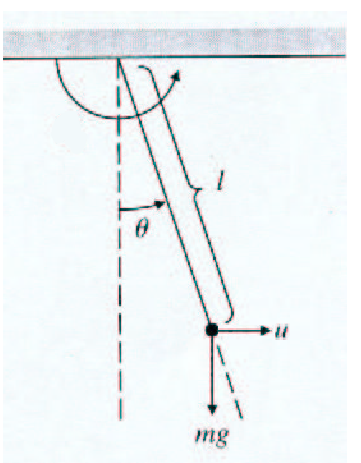
\includegraphics[width=0.3\textwidth]{./images/pendolo.png}
  \label{fig:pendolo}
  \caption{Schema di un pendolo\label{fig:pendolo}}
\end{figure}
Supponiamo di avere un pendolo di lunghezza $l$. L'asta del pendolo
\`e rigida. Alla baste dell'asta c'\`e una massa $m$. \`E presente un
attrito $B$. Le forze agenti
sono la forza applicata e la forza peso. Considereremo le componenti
tangenziali al moto e la componente dovuta all'attrito. Abbiamo che
l'ascissa curvilinea $s$ \`e pari a $s = l \theta$ e l'accelerazione
tangenziale \`e pari a $\ddot{s} = l \ddot{\theta}$. L'equazione del
moto \`e:
\begin{equation}
  u cos\theta - mg sin\theta - B \dot{\theta} = m l \ddot{\theta}
\end{equation}
cio\`e alla forza $u$ in ingresso si oppongono la gravit\`a (lungo
l'asse verticale) e l'attrito $B$.
Scriviamo la rappresentazione di stato ponendo $x_1 = \theta$ e $x_2 =
\dot{\theta}$:
\[
  \left\{
  \begin{array}{l}
    \dot{x_1} = x_2\\
    \dot{x_2} = \dfrac{1}{ml}\;u\;cos{x_1} - \dfrac{B}{ml}\;x_2 -
    \dfrac{g}{l}\;sin{x_1}
  \end{array}\right .
\]
Ponendo le derivate pari a zero, $x_2 = 0$ e, quindi, i punti di
equilibrio del sistema sono:
$$mg\sin{\overline{\theta}} = \overline{u}cos{\overline{\theta}}
\Rightarrow \overline{\theta} \;arctg
\left(\frac{\overline{u}}{mg}\right)$$
Se l'ingresso $\overline{u}$ di equilibrio \`e nullo si ottengono due
punti di equilibrio:
$\overline{\theta_1} = 0$ e $\overline{\theta_2} = \pi$.

\subsection{Carro-Ponte}
\begin{figure}[!h]
  \centering
  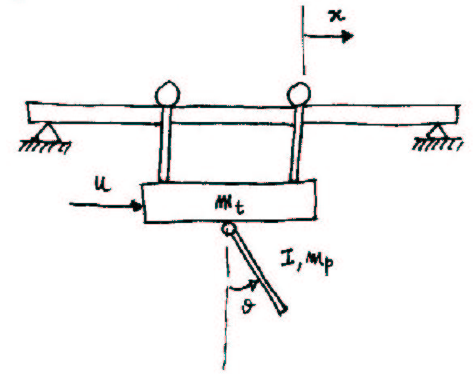
\includegraphics[width=0.5\textwidth]{./images/carroponte.png}
  \label{fig:carroponte}
  \caption{Schema di un carro-ponte\label{fig:carroponte}}
\end{figure}
Il Carro-Ponte \`e un sistema complesso che, per\`o, pu\`o essere diviso in due
sottosistemi che gi\`a abbiamo studiato: il carrello (\ref{carrello})
ed il pendolo (\ref{pendolo}).
\begin{figure}[!b]
  \centering
  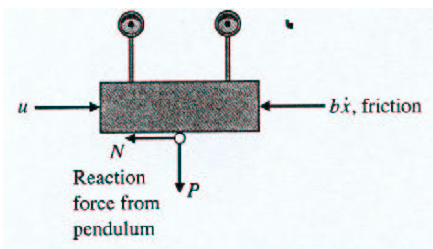
\includegraphics[width=0.5\textwidth]{./images/carroponte-carrello.png}
  \label{fig:carroponte-carrello}
  \caption{Schema di un carro-ponte: dettaglio del carrello\label{fig:carroponte-carrello}}
\end{figure}
Per il sottosistema ``carrello'', le equazioni sono quelle gi\`a
ampiamente discusse:
\begin{equation}\label{eq:carroponte-carrello}
  m_t \ddot{x} = u - N - b \dot{x}
\end{equation}
con lo spostamento $x$, l'attrito $b$ ed una sconosciuta forza di
reazione $N$ applicata dal pendolo.
Per il sottosistema del pendolo, le considerazioni sono leggermente diverse da
quelle fatte in precedenza poich\`e il fulcro del pendolo non \`e
fisso rispetto al sistema di riferimento inerziale: vanno considerate,
quindi, anche la rotazione del pendolo e lo spostamento del suo centro
di massa.
\begin{figure}[!h]
  \centering
  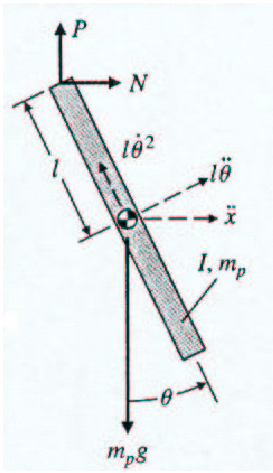
\includegraphics[width=0.3\textwidth]{./images/carroponte-pendolo-a.png}
  \label{fig:carroponte-pendolo-a}
  \caption{Schema di un carro-ponte: dettaglio del pendolo\label{fig:carroponte-pendolo-a}}
\end{figure}
La figura \ref{fig:carroponte-pendolo-a} mostra alcune delle
caratteristiche di questo sottosistema:
\begin{itemize}
\item $l \dot{\theta}^2$ \`e la componente accelerazione lungo il
  pendolo ed \`e detta {\em accelerazione
    centripeta}\index{Accelerazione centripeta} ed \`e presente in
  ogni oggetto la cui velocit\`a cambi direzione;
\item $\ddot{x}$ \`e una componente dell'accelerazione ed \`e una
  conseguenza del fulcro del pendolo che accelera a causa
  dell'accelerazione del carrello. Avr\`a sempre la stessa direzione e
  modulo di quella del carrello;
\item $l \ddot{\theta}$ \`e il risultato dell'accelerazione angolare
  del pendolo ed \`e sempre perpendicolare al pendolo stesso.
\end{itemize}
Questi risultati possono essere confermati considerando il centro di
massa del pendolo come un vettore, in riferimento ad un sistema di
riferimento inerziale, come mostrato in figura \ref{fig:carroponte-pendolo-b}.
\begin{figure}[!h]
  \centering
  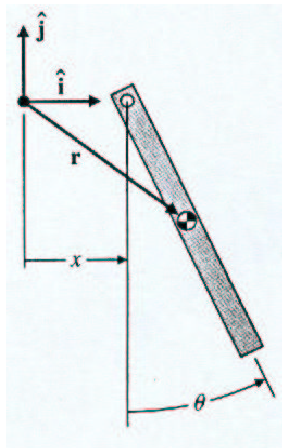
\includegraphics[width=0.3\textwidth]{./images/carroponte-pendolo-b.png}
  \label{fig:carroponte-pendolo-b}
  \caption{Schema di un carro-ponte: dettaglio del pendolo\label{fig:carroponte-pendolo-b}}
\end{figure}
La figura \ref{fig:carroponte-pendolo-b} mostra gli assi
$\hat{i}$ e $\hat{j}$, inerzialmente fissi e il vettore $\vec{r}$ che
descrive la posizione del centro di massa del pendolo. Il vettore
$\vec{r}$ pu\`o essere espresso come:
\[
  \vec{r} = x \hat{i} + l (\hat{i} sin \theta - \hat{j} cos \theta)
\]
Derivando otteniamo:
\[
\begin{array}{l}
  \dot{\vec{r}} = \dot{x} \hat{i} + l \dot{\theta} (\hat{i} cos \theta
  + \hat{j} sin \theta)\\
  \ddot{\vec{r}} = \ddot{x} \hat{i} + l \ddot{\theta} (\hat{i} cos
  \theta + \hat{j} sin \theta) - l \dot{\theta}^2 ( \hat{i} sin \theta
  - \hat{j} cos \theta)
\end{array}
\]
Abbiamo ottenuto tutte le equazioni del sistema. In teoria potremmo
applicare le equazioni per il moto traslatorio e rotatorio fino ad
ottenere tre equazioni in tre incognite: $N$, $P$ e $\theta$. Questo
sistema di equazioni pu\`o per\`o essere manipolato fino ad arrivare
ad una sola equazione in $\theta$:
\begin{equation}\label{eq:carroponte-N}
  N = m_p \ddot{x} + m_p l \ddot{\theta} cos \theta - m_p l
  \dot{\theta}^2 sin \theta
\end{equation}
Tuttavia possiamo limitare notevolmente i calcoli se applichiamo le
equazioni perpendicolarmete al pendolo:
\begin{equation}\label{eq:carroponte-P}
P sin \theta + N cos \theta - m_p g sin \theta = m_p l \ddot{\theta} +
m_p \ddot{x} cos \theta
\end{equation}
Applicando le equazioni intorno al centro di massa del pendolo
otteniamo:
\begin{equation}\label{eq:carroponte-I}
  - P l sin \theta - N l cos \theta = I \ddot{\theta}
\end{equation}
Combinando la \ref{eq:carroponte-N} e la \ref{eq:carroponte-carrello} otteniamo:
\begin{equation}
  (m_t + m_p) \ddot{x} + b \dot{x} + m_p l \ddot{\theta} cos \theta -
  m_p l \dot{\theta}^2 sin \theta = u
\end{equation}
Combinando la \ref{eq:carroponte-P} e la \ref{eq:carroponte-I}
otteniamo:
\begin{equation}
  (I + m_p l^2) \ddot{x} + m_p g l sin \theta = - m_p l \ddot{x} cos \theta
\end{equation}
Entrambe le equazioni sono non-lineari e vanno linearizzate per
piccoli spostamenti ($\theta = 0$). Supponiamo che $cos \theta
\cong 1$, $sin \theta \cong 0$ e $\dot{\theta}^2 \cong
0$. In questo modo le equazioni diventano:
\begin{equation}\label{eq:carroponte-nonlineare}
  \left\{
  \begin{array}{l}
    ( I + m_p l^2) \ddot{\theta} + m_p g l \theta = - m_p l \ddot{x}\\
    (m_t + m_p) \ddot{x} + b \dot{x} + m_p l \ddot{\theta} = u
  \end{array}
  \right .
\end{equation}
Trascurando l'attrito otteniamo la funzione di trasfermimento:
\begin{equation}
  \dfrac{\Theta(s)}{U(s)} = \dfrac{- m_p l}{((I + m_p l^2)(m_t + m_p)
    - m_p^2 l^2)s^2 + m_p g l (m_t + m_p)}
\end{equation}

\subsubsection{Pendolo inverso}\index{Pendolo inverso}
Nel caso del pendolo inverso, cio\`e considerando un carrello che si
muove su un piano e il fulcro del pendolo posto sul carrello le
considerazioni da fare sono diverse. Quando, in precedenza, abbiamo
assunto che $\theta \cong \pi$ assumiamo ora $\theta \cong \pi +
\theta'$, con $\theta'$ pari al movimento verso l'alto. In questo
caso, $cos \theta \cong -1$ e $sin \theta \cong - \theta'$ trasformano
la \ref{eq:carroponte-nonlineare} in:
\begin{equation}\label{eq:carroponte-pendoloinverso}
  \left\{
  \begin{array}{l}
    ( I + m_p l^2) \ddot{\theta'} - m_p g l \theta' = m_p l \ddot{x}\\
    (m_t + m_p) \ddot{x} + b \dot{x} - m_p l \ddot{\theta'} = u
  \end{array}
  \right .
\end{equation}
Come detto in precedenza, un sistema stabile ha sempre segni concordi
per le stesse variabili. Nelle equazioni precedenti notiamo che
$\theta'$ e $\ddot{\theta'}$ hanno segno opposto; ci\`o indica
``instabilit\`a'', che \`e la caratteristica principale del pendolo
inverso. La funzione di trasferimento, nuovamente ignorando l'attrito,
\`e: 
\begin{equation}
   \dfrac{\Theta'(s)}{U(s)} = \dfrac{m_p l}{((I + m_p l^2) - m_p^2
     l^2) s^2 - m_p g l (m_t + m_p)}
\end{equation}

\section{Sistemi elettrici}

\subsection{Legge di Kirchhoff ai nodi}
\begin{equation}\label{eq:kirchhoff-nodi}
  \sum_{i=1}^{N} I_k = 0
\end{equation}
La sommatoria delle correnti afferenti ad un nodo \`e nulla

\subsection{Legge di Kirchhoff alle tensioni}
\begin{equation}\label{eq:kirchhoff-tensioni}
  \sum v_{ij} = 0
\end{equation}
La sommatoria delle tensioni appartenenti ad una maglia \`e nulla.

\subsection{I principali elementi elettrici}

\begin{itemize}
  \item Il resistore
    $$ V_R = R i_R \Rightarrow V_R = R I_R$$
  \item Il condensatore
    $$ i_C = C \frac{dV_c}{dt} \Rightarrow V_C = \frac{1}{sC} I_C$$
  \item L'induttore
    $$V_L = L \frac{di_l}{dt} \Rightarrow V_L = sL I_L$$
\end{itemize}

\subsection{Sistemi elettromagnetici}

\begin{itemize}
  \item Una carica elettrica\index{Carica elettrica} $q$, in moto in un campo di induzione
    magnetica $B$ con velocit\`a $\vec{v}$, \`e soggetta ad una forza
    magnetica $$ \vec{F} = q \vec{v} \times \vec{B}$$
  \item Dato un filo rettilineo\index{Filo} di lunghezza $l$, percorso da corrente
    di intensit\`a $I$, immerso in un campo di induzione magnetica
    $B$, la forza magnetica agente sul filo \`e $$\vec{F} = I \vec{l}
    \times \vec{B}$$
  \item Data una spira\index{Spira} immersa in un campo di induzione
    magnetica $\vec{B}$ entrante, il flusso magnetico concatenato con
    la spira \`e $$\Phi_B = Blx$$ con $x$ pari alla distanza tra il
    lato sinistro della spira ed il limite del campo magnetico. Quando
    la spira si muove con velocit\`a $\vec{v}$ il flusso varia:
    $$\dot{\Phi}_B = Bl \dot{x} = -Blv$$
    Tale variazione di flusso produce una {\em forza
      elettromotrice}\index{Forza elettromotrice}
    $$e = Blv$$ sulla spira, che fa fluire nella spira stessa una
    corrente $I$.
\end{itemize}

\subsection{Circuito RLC}
\begin{figure}[!b]
\centering
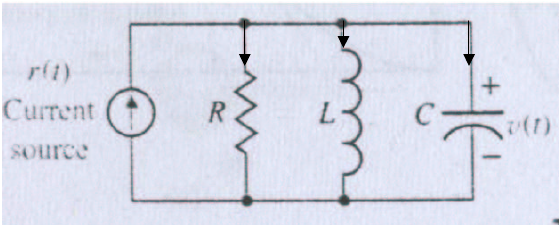
\includegraphics[width=0.5\textwidth]{./images/circuitorlc.png}
\caption{Circuito RLC\label{fig:circuitorlc}}
\end{figure}
Applicando le leggi di Kirchhoff (\ref{eq:kirchhoff-nodi} e
\ref{eq:kirchhoff-tensioni}) otteniamo le seguenti equazioni:
\[
  \left\{
  \begin{array}{l}
    i_L + i_R + i_C = r\\
    v_R = v_L = v_C = y
  \end{array}
  \right .
\]
Sostituendo le caratteristiche tensione-corrente per i singoli
elementi elettrici, si ottiene:
\[
  \left\{
  \begin{array}{l}
   \dfrac{y}{R} + i_L + C \dfrac{dv_C}{dt} = r\\
   y = L \dfrac{di_L}{dt}
  \end{array}
  \right .
\]
Derivando la prima equazione e sostituendo alla derivata di $i_L$ la
seconda equazione, se ne ricava una finale pari a:
\[
  \ddot{y} + \dfrac{\dot{y}}{RC} + \dfrac{y}{LC} = \dfrac{\dot{r}}{C}
\]
Sostituendo $s$ a $\dfrac{d}{dt}$ possiamo ottenere la funzione di
trasferimento: 
\[
  \begin{array}{l}
    \ddot{y} + \dfrac{\dot{y}}{RC} + \dfrac{y}{LC} =
    \dfrac{\dot{r}}{C}\\
    s^2 Y + \dfrac{sY}{RC} + \dfrac{Y}{LC} = \dfrac{sr}{C}\\
    Y(s^2 + \dfrac{s}{RC} + \dfrac{1}{LC}) = \dfrac{sr}{C}\\
  \end{array}
\]
\begin{equation}\label{eq:fdt-circuitorlc}
  G(s) = \dfrac{1}{sC + \dfrac{1}{R} + \dfrac{1}{sL}}
\end{equation}
Per ottenere la rappresentazione in forma di stato, poniamo $i_L =
x_1$, $v_C = x_2$:
\[
  \left\{
  \begin{array}{l}
    \dot{x}_1 = \dfrac{x_2}{L}\\
    \dot{x}_2 = - \dfrac{x_1}{C} - \dfrac{x_2}{RC} + \dfrac{r}{C}\\
    y = x_2
  \end{array}
  \right .
\]


\subsection{Amplificatore operazionale}
\begin{figure}[!b]
\centering
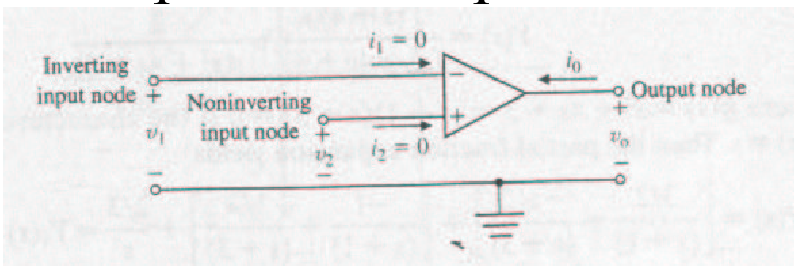
\includegraphics[width=0.8\textwidth]{./images/opamp.png}
\caption{Amplificatore operazionale\label{fig:opamp}}
\end{figure}
\`E un elemento attivo e fornisce un alto guadagno nella regione di
funzionamento lineare. L'amplificatore ideale ha le seguenti principali
propriet\`a:
\begin{itemize}
\item $i_1 = i_2 = 0$ cio\`e la corrente entrante nell'amplificatore
  \`e nulla, quindi si ha una impedenza d'ingresso infinita;
\item $v_2 - v_1 = 0$ cio\`e il corto circuito virtuale tra i due
  morsetti d'ingresso;
\item $R_1 = \infty$, $R_O = 0$ e $K = \infty$;
\end{itemize}
Il legame ingresso-uscita \`e quindi:
\[
  v_O = - K (v_1 - v_2)
\]
\subsubsection{Configurazione invertente}
\begin{figure}[!t]
\centering
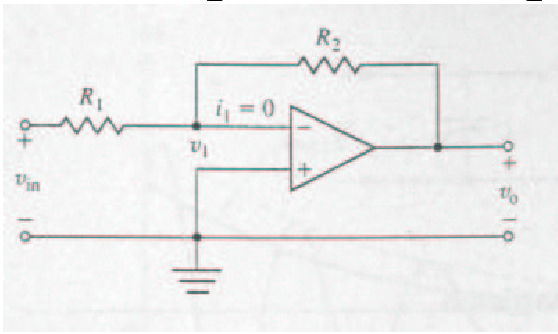
\includegraphics[width=0.5\textwidth]{./images/opamp02.png}
\caption{Amplificatore operazionale in configurazione invertente\label{fig:opamp-inv}}
\end{figure}
Il generatore \`e collegato al morsetto ``-'' e il morsetto ``+'' \`e
posto a massa:
\[
  \begin{array}{c}
    \dfrac{v_1 - v_{in}}{R_1} + \dfrac{v_1 - v_o}{R_2} = 0\\
    \textrm{ che con } v_1 - v_2 = 0 \textrm{ e } v_2 \textrm{ a massa
    ci porta a }\\
    -\dfrac{v_{in}}{R_1} = \dfrac{v_o}{R_2}\\
    \Downarrow\\
    \dfrac{v_o}{v_{in}} = -\dfrac{R_2}{R_1}
  \end{array}
\]

\subsubsection{Integratore di Miller}\index{Integratore di Miller}
\begin{figure}[!h]
\centering
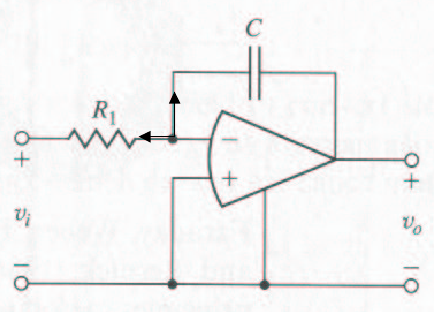
\includegraphics[width=0.5\textwidth]{./images/opamp03.png}
\caption{Amplificatore operazionale - Integratore di Miller\label{fig:opamp-mil}}
\end{figure}
Date le propriet\`a dell'amplificatore ideale, si ha:
\[
  \left\{\begin{array}{l}
    i_c = C \dfrac{d(v_1 - v_o)}{dt}\\
    i_R = \dfrac{v_1 - v_{in}}{R}
  \end{array}\right .
  \Rightarrow - \dfrac{v_{in}}{R} - C \dfrac{dv_o}{dt} = 0
\]
\[
  - \int\dfrac{v_{in}}{R} = \int C \dfrac{dv_o}{dt} \Rightarrow
\]
\[
  - \dfrac{1}{RC}\int\limits_0^t v_{in}(\tau)d\tau = v_o(t) - v_o(0)
\]
Ecco l'integratore:
\[
  v_o(t) = - \dfrac{1}{RC}\int\limits_0^t v_{in}(\tau)d\tau + v_o(0)
\]
La funzione di trasferimento \`e:
\[
  \dfrac{V_O (s)}{V_{in} (s)} = G (s) = - \dfrac{1}{sRC}
\]

\subsection{Forza magnetica}
\begin{figure}[!h]
\centering
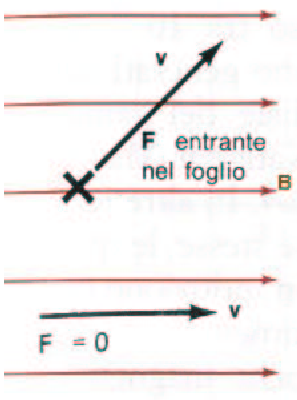
\includegraphics[width=0.2\textwidth]{./images/forza-magnetica.png}
\caption{Forza magnetica\label{fig:forza-magnetica}}
\end{figure}
Una carica elettrica $q$, in moto in un campo di induzione magnetica $B$ con
velocità $v$, \`e soggetta ad una forza magnetica
\begin{equation}\label{eq:forza-magnetica}
  \vec{F} = q \vec{v} \times \vec{B}
\end{equation}
Il modulo di $F$ \`e $q v B sin \theta$, il verso \`e perpendicolare a
$v$ e $B$ e si calcola con la regola della mano destra.

\subsubsection{Forza magnetica su un filo conduttore}
\begin{figure}[!h]
\centering
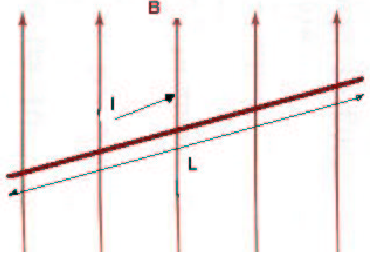
\includegraphics[width=0.2\textwidth]{./images/forza-magnetica02.png}
\caption{Forza magnetica su un filo conduttore\label{fig:forza-magnetica02}}
\end{figure}
Dato un filo rettilineo di lunghezza $L$, percorso da corrente di
intensit\`a $I$, immerso in un campo di induzione magnetica $B$, la
forza magnetica agente sul filo \`e:
\begin{equation}\label{eq:forza-magnetica-filo}
  \vec{F} = I \vec{L} \times \vec{B}
\end{equation}

\subsubsection{Forza elettromotrice indotta}
\begin{figure}[!h]
\centering
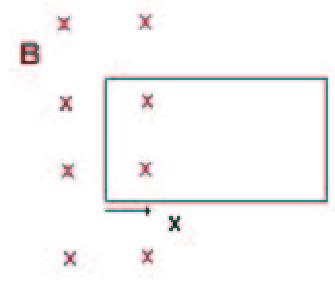
\includegraphics[width=0.3\textwidth]{./images/forza-magnetica03.png}
\caption{Forza elettromotrice indotta\label{fig:forza-magnetica03}}
\end{figure}
Data una spira immersa in un campo di induzione magnetica $B$
entrante, il flusso magnetico concatenato con la spira
\[
  \Phi_B = B l x
\]
dove $x$ \`e la distanza tra il lato sinistro della spira e il limite
destro del campo magnetico. Quando la spira si muove con velocit\`a
$v$, il flusso varia:
\[
  \dot{\Phi}_B = B l \dot{x} = - B l v
\]
Tale variazione di flusso produce una forza elettromotrice 
\[
  e(t) = B l v
\]
sulla spira, che  fa fluire nella spira stessa una corrente $I$.
\subsubsection{Forza contro-elettromotrice}
\begin{figure}[!h]
\centering
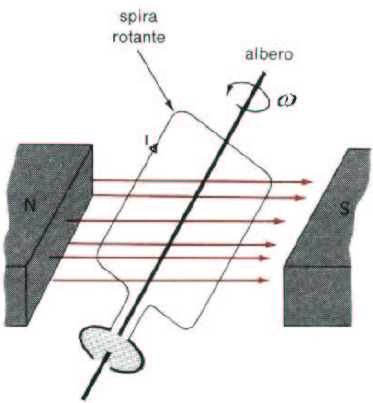
\includegraphics[width=0.3\textwidth]{./images/forza-magnetica04.png}
\caption{Forza contro-elettromotrice\label{fig:forza-magnetica04}}
\end{figure}
Una spira percorsa da corrente $I$, che ruota in un campo di induzione
magnetica $B$ con velocit\` angolare $\omega$ il flusso magnetico
concatenato con la spira è
\[
  \Phi_B = B l sin \alpha
\]
con $\alpha$ pari all'angolo formato dalla spira con il campo $B$. Al
ruotare della spira, il flusso varia:
\[
  \dot{\Phi}_B = B l x \dot{\alpha} cos \alpha = - B l x \omega cos \alpha
\]
La forza elettromotrice indotta, pari a
\[
  e = B l x \omega cos \alpha
\]
si oppone alla tensione d'alimentazione della spira ed \`e detta {\em
  forza contro-elettromotrice}.

\subsection{Altoparlante}
\begin{figure}[!h]
\centering
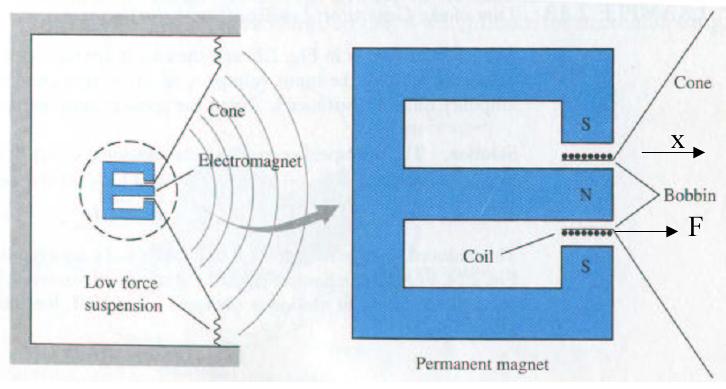
\includegraphics[width=0.5\textwidth]{./images/altoparlante.png}
\caption{Altoparlante\label{fig:altoparlante}}
\end{figure}
L'altoparlante \`e composto da $N$ spire di lunghezza $l$ avvolte
intorno al polo $N$ dell'elemento ferromagnetico. Le spire sono
attraversate dalla corrente $i$. Il campo di induzione magnetica \`e
$B$. La forza magnetica che agisce sulle spire \`e:
\[
  F = N l i B
\]
Questa forza induce le spire ad un movimento orizzontale. Durante il
loro movimento, le spire, di massa $M$, incontrano un attrico viscoso $b$ imposto
dall'ambiente. Applicando la Legge di Newton (\ref{leggedinewton})
abbiamo:
\begin{equation}\label{eq:amplificatore}
  M \ddot{x} + b \dot{x} = F
\end{equation}
\begin{figure}[!h]
\centering
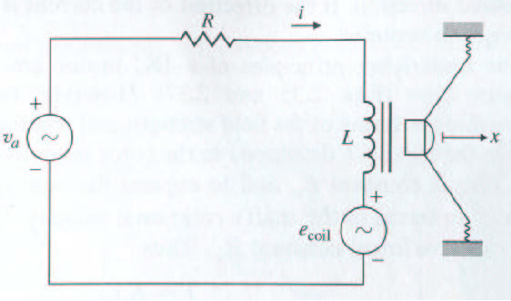
\includegraphics[width=0.5\textwidth]{./images/altoparlante02.png}
\caption{Altoparlante e circuito di alimentazione\label{fig:altoparlante02}}
\end{figure}
Consideriamo il circuito con cui sono alimentate le spire (figura
\ref{fig:altoparlante02}). Questo circuito avr\`a una sua resistenza
$R$ ed una induttanza $L$. \`E presente anche un generatore di
tensione $v_a$. Lo spostamento delle spire nel campo $B$ produce una
forza contro-elettromotrice
\[
  e = B l v
\]
dove $v = \dot{x}$. L'equazione alla maglia di alimentazione \`e:
\begin{equation}\label{eq:Altoparlante-circuito}
  L \dfrac{di}{dt} + Ri = v_a - e
\end{equation}

\subsection{Motore in corrente continua}
\begin{figure}[!t]
\centering
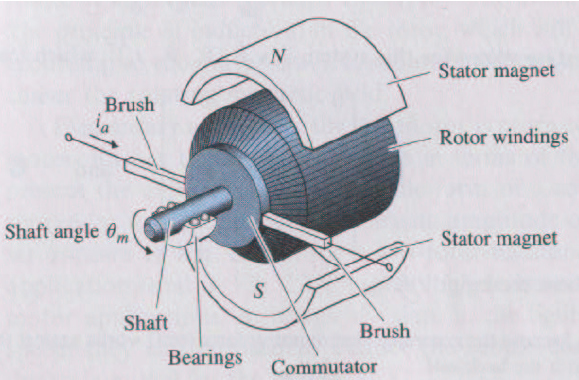
\includegraphics[width=0.5\textwidth]{./images/motoreDC.png}
\caption{Motore in corrente continua\label{fig:motoreDC}}
\end{figure}
Lo statore di figura \ref{fig:motoreDC} pu\`o essere di materiale ferromagnetico, oppure un magnete
permanente. Il rotore \`e avvolto, parallelamente al suo asse di
rotazione, da $N$ bobine. Le bobine sono alimentate a turno da un
commutatore e due spazzole, alle quali arriva la corrente $i$ dal
circuito di alimentazione. All'albero motore si collega un carico, che
viene messo in rotazione dal motore.
\begin{figure}[!t]
\centering
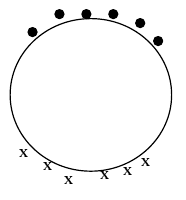
\includegraphics[width=0.2\textwidth]{./images/motoreDC02.png}
\caption{Motore in corrente continua - Vista frontale\label{fig:motoreDC02}}
\end{figure}
La corrente entra in ogni bobina nella parte superiore del rotore ed
esce da quella inferiore. Su ogni bobina agisce la  forza magnetica
\[
F=Bli
\]
dal lato in ingresso della corrente e dal lato in uscita. La coppia
prodotta su ciascuna bobina \`e:
\[
  T = F r sin \alpha
\]
\begin{figure}[!t]
  \centering
  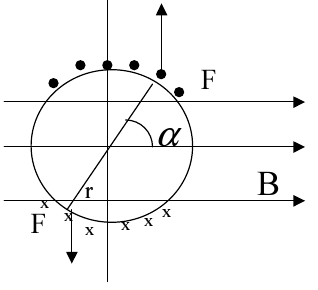
\includegraphics[width=0.3\textwidth]{./images/motoreDC03.png}
  \caption{Motore in corrente continua - Vista frontale dettagliata
    \label{fig:motoreDC03}}
\end{figure}
La coppia prodotta sul rotore dipende dall'angolo $\alpha$ (figura
\ref{fig:motoreDC03}): usando $N$ 
bobine avvolte al rotore, la coppia totale sar\`a una media di tutte
le coppie applicate alle singole bobine e sar\`a eliminata la dipendenza da
$\alpha$. La coppia complessiva sar\`a
\[
  T = K_t i_a
\]
con $K_t$ costante di coppia ed $i_a$ corrente nelle
armature. 

Analogamente si pu\`o vedere che ogni bobina alimentata subisce una
forza contro-elettromotrice dipendente dalla velocit\`a angolare
$\dot{\theta}_m$ del motore e da $\alpha$. La forza
contro-elettromotrice complessiva \`e
\[
  e = K_e \dot{\theta}_m
\]
con $K_e$ equivalene elettrica della costante di coppia $K_t$ e
$\dot{\theta}_m$ velocit\`a di rotazione dell'albero motore.
\begin{figure}[!t]
\centering
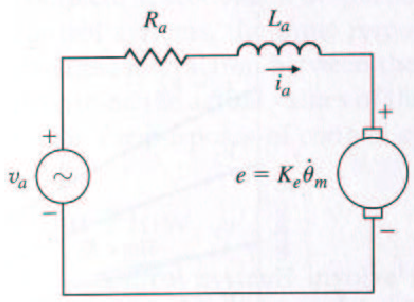
\includegraphics[width=0.5\textwidth]{./images/motoreDC04.png}
\caption{Circuito di alimentazione del motore DC\label{fig:motoreDC04}}
\end{figure}
Consideriamo il circuito di alimentazione del motore di figura
\ref{fig:motoreDC04}: esso \`e costituito da un generatore di tensione
$v_a$, una resistenza $R_a$ ed un'induttanza $L_a$. L'equazione di
tale circuito \`e:
\[
  L_a \dfrac{di_a}{d_t} + R_a i_a + K_e \dot{\theta} = v_a
\]
\begin{figure}[!b]
\centering
\includegraphics[width=0.3\textwidth]{./images/motoreDC05.png}
\caption{Motore DC - Parte meccanica\label{fig:motoreDC05}}
\end{figure}
Per quanto riguarda la parte meccanica del motore (figura
\ref{fig:motoreDC05}), se sull'asse del rotore si pone un carico di
inerzia $J_l$, la Legge di Newton (\ref{leggedinewton}) ci porta alle equazioni:
\[
  \begin{array}{l}
    J_m \ddot{\theta}_m + b( \dot{\theta}_m - \dot{\theta}_l) + k
    (\theta_m - \theta_l) = K_t i_a\\
    J_l \ddot{\theta}_l + b( \dot{\theta}_l - \dot{\theta}_m) + k
    (\theta_l - \theta_m) = 0
  \end{array}
\]
Per qualche approfonfimento sul moto rotatorio fate riferimento al
paragrafo \ref{par:discorotanteattrito}.



\section{Dinamica dei fluidi}
Le relazioni fisiche che governano i flussi di fluidi sono la
continuit\`a, l'equilibrio tra le forze e la resistenza. La relazione
di continuit\`a \`e semplicemente una dichiarazione di conservazione
della materia:
\begin{equation}\label{eq:conservazione-massa}
  \dot{m} = \omega_{in} - \omega_{out}
\end{equation}
dove
\begin{itemize}
\item $m$ = massa del fluido
\item $\omega_{in}$ = portata dell'ingresso
\item $\omega_{out}$ = portata dell'uscita
\end{itemize}

\subsection{Serbatoio}
\begin{figure}[!h]
\centering
\includegraphics[width=0.5\textwidth]{./images/serbatoio.png}
\caption{Serbatoio\label{fig:serbatoio}}
\end{figure}
Nel caso di un semplice contenitore, applicando la
\ref{eq:conservazione-massa} otteniamo l'equazione del {\em moto
  fluidi per i serbatoi}\index{Serbatoio}\index{Serbatoio}:
\begin{equation}\label{eq:fluidi-serbatoio}
  \dot{h} = \frac{\omega_{in} - \omega_{out}}{A \rho}
\end{equation}
dove
\begin{itemize}
\item $A$ \`e l'area del serbatoio;
\item $\rho$ \`e la densit\`a del fluido;
\item $h = \dfrac{m}{A \rho}$ \`e l'altezza dell'acqua;
\item $A \rho$ definisce la quantit\`a di fluido, in litri, che
  attraversa la sezione;
\item $m$ \`e la massa di acqua nel serbatoio.
\end{itemize}

\subsection{Pistone idraulico}
\begin{figure}[!h]
\centering
\includegraphics[width=0.5\textwidth]{./images/pistone.png}
\caption{Pistone\label{fig:pistone}}
\end{figure}
Considerata una forza $F_D$ che aziona un pistone idraulico ed una
pressione $p$ nella camera del pistone, possiamo applicare la
\ref{leggedinewton} e la sua equivalente per i fluidi:
\begin{equation}\label{eq:newton-fluidi}\index{Legge di Newton per i fluidi}
  f = p A
\end{equation}
dove
\begin{itemize}
\item $f$ \`e la forza;
\item $p$ \`e la pressione;
\item $A$ \`e l'area della superficie contro cui il fluido preme
\end{itemize}
Ne consegue l'equazione del moto del pistone:
\begin{equation}\label{eq:pistone}
  M\ddot{x} = A \cdot p - F_D
\end{equation}
dove
\begin{itemize}
\item $A$ \`e l'area del pistone;
\item $p$ \`e la pressione della camera;
\item $M$ \`e la massa del pistone;
\item $x$ \`e la posizione del pistone.
\end{itemize}

\subsection{Flusso attraverso un orifizio}\index{Orifizio}
Se nel corso del suo flusso, il liquido incontra una restrizione
(pu\`o essere rappresentata da un orifizio o da una valvola, figura \ref{fig:orifizio}), la
pressione varia e quindi anche il flusso:
\begin{equation}\label{eq:orifizio}
  \omega = \frac{1}{R} (p_1 - p_2)^{\frac{1}{\alpha}}
\end{equation}
dove
\begin{itemize}
\item $p_1$ \`e la pressione prima della costrizione;
\item $p_2$ \`e la pressione dopo la costrizione;
\item $R$ \`e la resistenza idrica;
\item $\omega$ \`e la portata di fluido che passa per la costrizione.
\end{itemize}
Tipicamente si pone $\alpha = 1$ se il condotto \`e lungo e il flusso
\`e laminare e lento. Diversamente $\alpha = 2$ se il condotto \`e
corto e il flusso \`e turbolento. Noi supporremo sempre $\alpha = 2$.

\subsection{Attuatore idraulico}
\begin{figure}[!b]
\centering
\includegraphics[width=0.9\textwidth]{./images/attuatoreidraulico.png}
\caption{Attuatore idraulico\label{fig:attuatoreidraulico}}
\end{figure}
``In senso lato, un attuatore \`e talvolta definito come un qualsiasi
dispositivo che converte dell'energia da una forma ad un'altra, in
modo che questa agisca nell'ambiente fisico al posto dell'uomo.'' -
Wikipedia 

L'ingresso di controllo \`e $x$, il segnale di attuazione \`e
$y$. Supponendo i flussi attraverso gli orifizi proporzionali ad $x$:
\[
  \omega_1 = \dfrac{1}{R_1} (p_s - p_1)^{1/2}x
\]
\[
  \omega_2 = \dfrac{1}{R_2} (p_2 - p_e)^{1/2}x
\]
Applicando la relazione di continuit\`a otteniamo:
\begin{equation}
  \rho A \dot{y} = \omega_1 = \omega_2
\end{equation}
dove $A$ \`e l'area del pistone e $\rho$ \`e la densit\`a del
liquido. In aggiunta definiamo il bilancio delle forze sul pistone
come:
\begin{equation}
  A (p_1 - p_2) - F = m \ddot{y}
\end{equation}
dove $F$ \`e la forza applicata all'asta del pistone dal punto di
aggancio del sistema controllato. L'equazione del moto del sistema
controllato \`e:
\begin{equation}
  I \ddot{\theta} = F l cos \theta - F_a d
\end{equation}
dove $F_a$ \`e la forza dovuta al carico aerodinamico.

\subsection{Esempio di serbatoio con costrizione}
\begin{figure}[!t]
\centering
\includegraphics[width=0.5\textwidth]{./images/orifizio.png}
\caption{Orifizio\label{fig:orifizio}}
\end{figure}
Abbiamo gi\`a visto che per l'altezza $h$ vale la legge:
\begin{equation}
  \dot{h} = \dfrac{\omega_{in} - \omega_{out}}{A \rho}
\end{equation}
In questo caso c'\`e per\`o una restrizione, come nel punto di uscita
in figura \ref{fig:serbatoio}, che ci porta a riscrivere
la relazione:
\begin{equation}
  \omega_{out} = \dfrac{1}{R} \left(p_i - p_a \right)^{\frac{1}{2}}
\end{equation}
con
\begin{equation}
  p_i = \rho g h + p_a
\end{equation}
con $p_i$ pressione dell'acqua e $p_a$ pressione
dell'ambiente. Sostituendo, si ottiene:
\begin{equation}
  \dot{h} = \dfrac{1}{A \rho} \left(\omega_{in} - \dfrac{1}{R}\sqrt{\rho g h}\right)
\end{equation}
\subsubsection{Punto di equilibrio}
Dato un $\overline{\omega}_{in}$ costante, se esiste un punto di
equilibrio deve essere $\overline{h}$ costante:
\[
  0 = \dfrac{1}{A \rho} \left( \overline{\omega}_{in} -
  \dfrac{1}{R}\sqrt{\rho g \overline{h}} \right) \Rightarrow
  \overline{\omega}_{in} = \dfrac{\sqrt{\rho g \overline{h}}}{R}
  \Rightarrow \overline{h} = \dfrac{R^2 \cdot \omega_{in}^2}{\rho g}
\]
\subsubsection{Linearizzazione intorno ad $\overline{h}$}
\[
  \begin{array}{l}
    \omega_{in} = \overline{\omega}_{in} + \delta \omega_{in}\\
    h = \overline{h} + \delta h\\
    \delta \dot{h} = \dfrac{1}{\rho A} (\overline{\omega}_{in} + \delta
    \omega_{in}) - \dfrac{1}{\rho AR}\sqrt{\rho g (\overline{h} +
      \delta h)}
  \end{array}
\]
Sviluppando in serie di $\sqrt{\overline{h} - \delta h}$ con $\delta h
\rightarrow 0$ si ha:
\[
  \sqrt{\overline{h}} + \left . \frac{1}{2} \cdot \dfrac{1}{\sqrt{\overline{h}
      + \delta h}}\right|_{\delta h \rightarrow 0} \cdot \delta h =
  \sqrt{\overline{h}} + \frac{1}{2} \dfrac{\delta h}{\sqrt{\overline{h}}}
\]
Sostituendo si ottiene l'equazione lineare in $\delta h$:
\[
  \delta \dot{h} = \dfrac{1}{\rho A} \delta \omega_{in} =
  \dfrac{\sqrt{g} \delta h}{\sqrt{\rho \overline{h}} \cdot 2 AR}
\]

\section{Scambio termico}
\begin{figure}[!h]
  \centering
  \includegraphics[width=0.4\textwidth]{./images/scambiotermico01.png}
  \caption{Scambio termico\label{fig:scambiotermico01}}
\end{figure}
Abbiamo due ambienti separati da una parete, la quale lascia passare
il calore. La quantit\`a di calore $q$ che viene scambiata attraverso
la parete \`e:
\begin{equation}
  q = \frac{1}{R} (T_1 - T_2)
\end{equation}
$R$ \`e la resistenza termica della parete, $T_1$ \`e la temperatura
dell'ambiente 1 e $T_2$ quella dell'ambiente 2. Se $T_1 > T_2$, il flusso
di calore si muove dall'ambiente $1$ all'ambiente $2$. In generale
questa relazione vale nel caso in cui il passaggio di calore non
modifichi in modo significativo la temperatura. Per la variazione di
temperatura $\Delta T$ si pu\`o fare riferimento ad un'altra relazione:

\begin{equation}
\dot{T} = \frac{1}{C}q
\end{equation}
con $C$ capaticit\`a termica. La capaticit\`a termica \`e quel flusso
di calore necessario da applicare in ingresso ad un sistema per
determinare una variazione unitaria della temperatura.

\subsection{Temperatura in una stanza}
Consideriamo una stanza con tutti i lati isolati tranne due, i quali
scambiano calore con l'esterno. Detta $T_i$ la temperatura interna,
$T_o$ quella esterna e $C$ la capaticit\`a termica dell'aria
all'interno della stanza, si ha:
\begin{equation}
  \dot{T} = \frac{1}{C} \left[ \frac{1}{R_1}(T_o - T_i) +
    \frac{1}{R_2}(T_o - T_i) \right] 
\end{equation}
dove $R_1$ ed $R_2$ sono pari alle resistenze delle pareti al passaggio del
calore, $q_{in}$ \`e la quantit\`a di calore che la stanza
``acquista'', $q_{out}$ \`e la quantit\`a di calore che la stanza ``cede''
ad un ambiente pi\`u freddo. L'esercizio 2.25 del Franklin-Powell offre un interessante
esempio di applicazione di questi concetti. Il cardine di tutta
la risoluzione \`e l'analisi del comportamento del calore in relazione
ad ogni singola parete. Il calore muove sempre dall'ambiente pi\`u caldo all'ambiente
pi\`u freddo. Va, quindi, valutata la temperatura interna della stanza
e valutata l'eventualit\`a che la stanza sia collegata ad una stanza
pi\`u fredda o pi\`u calda, cio\`e che ``ceda'' o ``acquisti'' calore.

\subsection{Fluidi che si mescolano}
Il calore pu\`o anche fluire quando una massa pi\`u calda si mescola
con una pi\`u fredda. In questo caso:
\begin{equation}
  q = W C_s (T_1 - T_2)
\end{equation}
con $C_s$ calore specifico a volume costante e $W$ portata ponderale a
temperatura $T_1$ che flusce nel serbatoio a $T_2$.

\section{Esempi dalle prove d'esame}
\subsection{Sistema di riscaldamento elettrico}
Si supponga che un sistema di riscaldamento elettrico sia
schematizzabile come in figura \ref{fig:esempio01}: la tensione $v$
alimenta il circuito di riscaldamento e la potenza dissipata sul
resistore $R_2$ \`e integralmente trasformata in flusso di calore
immesso nell'ambiente $A$, il quale, a sua volta, pu\`o scambiare
calore con l'ambiente esterno attraverso la parete $S$. Assunto che:
\begin{itemize}
  \item[a)] $T$ indichi la temperatura interna dell'ambiente $A$, $T_E$
  quella dell'ambiente esterno, $C_T$ sia la capacit\`a termica del
  flusso in $A$ ed $r$ la resistenza termica della parete $S$;
  \item[b)] il calore scambiato tra l'ambiente $A$ e l'ambiente
    esterno attraverso $S$ non modifichi sensibilmente $T_E$ (in altre
    termini, si consideri $T_E$ costante);
  \item[c)] il resistore $R_2$ abbia resistenza elettrica dipendente
    dalla temperatura secondo la legge: $R_2 = R_0 + \alpha \cdot T$;
  \item[d)] la relazione tra flusso di calore $q$ e potenza $p$ sia $q
    = b \cdot p$ con $b$ costante nota;
\end{itemize}

Si chiede di:
\begin{itemize}
\item fornire una rappresentazione i-s-u per il sistema assegnato;
\item determinare il valore della tensione di alimentazione $v$
  (supposto $> 0$) da assegnare affinch\`e la temperatura in $A$
  rimanga in equilibrio al valore $T = 10^{\circ}C$;
\item linearizzare il modello sopra determinato intorno al punto di
  equilibrio sopra calcolato;
\end{itemize}
$[R_0 = 1 k\Omega; R_1 = 9 k\Omega; \alpha = 2 kW/^{\circ}C; C = 1 mF; C_T = 1
  cal/^{\circ}C; r = 2 ^{\circ}C \cdot sec/cal; T_E= 4 ^{\circ}C; b = 1
  cal/J]$
\begin{figure}[!h]
  \centering
  \includegraphics[width=0.7\textwidth]{./images/esempio01.png}
  \label{fig:esempio01}
  \caption{Sistema di riscaldamento elettrico\label{fig:esempio01}}
\end{figure}

\subsubsection{Equazioni del circuito}
\[
v = v_1 + v_2 = R_1(i_C + i_2) + v_2 = R_1 \left(C \frac{dv_2}{dt} +
\frac{v_2}{R_2}\right) + v_2
\]
\[
  v = R_1C\dot{v_2} + \left( \frac{R_1}{R_2} + 1\right)v_2 \Rightarrow
  \dot{v_2} = - \left( \frac{1}{R_1C} + \frac{1}{R_2C}\right)v_2 + \frac{1}{R_1C}v
\]
Essendo $R_2 = R_0 + \alpha T$ si ha:
\[
  \dot{v_2} = - \left( \frac{1}{R_1C} + \frac{1}{C(R_0 + \alpha T)}\right)v_2 + \frac{1}{R_1C}v
\]

\subsubsection{Equazioni di scambio termico}
\[
  \begin{array}{ll}
    \dot{T} = \dfrac{1}{C_T} (q_{in} - q_{out}) &  \\
    q_{in} = b i_2 v_2 = b \dfrac{v_2^2}{R_2} = \dfrac{b v^2}{R_0 +
      \alpha T} & \textrm{Flusso di calore in ingresso}\\
    q_{out} = \dfrac{1}{r}(T - T_E) & \textrm{Flusso di calore in
      uscita}\\
     & \\
    \dot{T} = \dfrac{b}{C_T} \cdot \dfrac{v_2^2}{R_0 + \alpha T} -
    \dfrac{1}{C_T r}T + \dfrac{1}{C_T r}T_E & 
  \end{array}
\]
\\
Posto: $x = v_1$ ; $x_2 = T$ ; $u = v$ ; $y = T$ si ha:
\[
  \begin{array}{l}
    \dot{x_1} = - \left( \dfrac{1}{R_1C} + \dfrac{1}{C R_0 + \alpha C
      x_2}\right)x_1 + \dfrac{1}{R_1 C}u\\
    \dot{x_2} = \dfrac{b}{C_T} \dfrac{x_1^2}{R_0 + \alpha x_2} -
    \dfrac{1}{C_T r}x_2 + \dfrac{1}{C_T r}T_E\\
    y = x_2
  \end{array}
\]
Sostituendo ai parametri i valori numerici assegnati si ha:
\[
  (S)
  \left\{
  \begin{array}{l}
    \dot{x_1} = - \left( \dfrac{1}{9} + \dfrac{1}{1 + 2x_2}\right)x_1 + \dfrac{1}{9}u\\
    \dot{x_2} = \dfrac{x_1^2}{1 + 2x_2} - \dfrac{1}{2}x_2 + 2\\
    y = x_2
  \end{array}
  \right .
\]
\\
Affinch\`e la temperatura $T = x_2$ sia in equilibrio a $10 ^{\circ}C$
deve essere soddisfatto l'equilibrio:

\[
  \begin{array}{ll}
    (1) & 0 = - \left( \frac{1}{9} + \frac{1}{1 + 2x_2}\right)x_1 +
    \frac{1}{9}u\\
    (2) & 0 = \frac{x_1^2}{1 + 2x_2} - \frac{1}{2}x_2 + 2\\
  \end{array}
\]
Sostituendo $x_2 = 10 ^{\circ}C$ si ha dalla (2):
\[
  \dfrac{\overline{x_1}^2}{21} - 5 + 2 = 0 \Rightarrow \overline{x_1}^2
  = 63 \Rightarrow \overline{x_1} = 
  \left\{
  \begin{array}{l}
    -3 \sqrt{7}\\
    +3 \sqrt{7}
  \end{array} \right .
\]
Dalla (1) invece si ha: $$\overline{u} = \left(1 +
\frac{9}{21}\right)\overline{x_1}$$
Poich\`e deve essere $\overline{u} > 0$, si ha: $$ \overline{u} =
\frac{30}{21} \cdot (+3\sqrt{7}) = \frac{30}{\sqrt{7}}$$
Si procede quindi alla Linearizzazione del sistema (S) intorno al
punto di equilibrio sopra determinato $(\overline{x_1},
\overline{x_2}, \overline{x_3}) = \left(+3\sqrt{7}, +10, \frac{30}{\sqrt{7}}\right)$

\[
  \left\{
  \begin{array}{l}
    \delta \dot{x_1} = - \left( \frac{1}{9} + \frac{1}{1 +
      2\overline{x}_2}\right)\delta x_1 + \frac{1}{(1 +
      2\overline{x}_2)^2}\delta x_2 + \frac{1}{9} \delta u\\
    \delta \dot{x_2} = \frac{2 \overline{x}_1}{1 + 2 \overline{x}_2}
    \delta x_1 + \left( - \frac{2 \overline{x}_1^2}{(1 + 2
      \overline{x}_2)^2} - \frac{1}{2} \right) \delta x_2\\
    \delta y = \delta x_2
  \end{array}
  \right .
\]

\subsection{Serbatoio su carrello con molla e smorzatore}
\begin{figure}[!b]
  \centering
  \includegraphics[width=0.5\textwidth]{./images/esempio02.png}
  \caption{Serbatoio su carrello con molla e smorzatore\label{fig:esempio02}}
\end{figure}
Si fornisca una rappresentazione i-s-u per il sistema riportato in
figura \ref{fig:esempio02}. Esso \`e costituito da un serbatoio con area
di base $A$ posto su un carrello di massa trascurabile. Il
collegamento tra la parete ed il serbatoio avviene mediante una molla
lineare (di costante elastica $k_1$) ed un ammortizzatore lineare (di
costante $b_1$). Il serbatoio \`e sottoposto alla forza di trazione
$F$. Si supponga che:
\begin{itemize}
\item nel serbatoio sia immesso un fluido avente densit\`a $\rho$ con
  portata massica $\omega_{in}$. Lo stesso fluido fuoriesca in
  condizioni di moto turbolento dall'orifizio con resistenza idrica
  $R$;
\item la forza $F$ sia l'uscita del sistema rappresentato in
  figura \ref{fig:esempio02-2} mediante schema a blocchi;
\item l'effetto del moto traslatorio sia trascurabile sia sulla
  fuoriuscita del fluido che sulla sua distribuzione all'interno del
  serbatoio; 
\item nello schema di figura \ref{fig:esempio02-2}, $G_1$ e $G_2$ siano
  due costanti di guadagno;
\item l'uscita del sistema complessivo sia lo spostamento dell'insieme
  carrello+serbatoio.
\end{itemize}
\begin{figure}[!b]
  \centering
  \includegraphics[width=0.5\textwidth]{./images/esempio02-2.png}
  \caption{Serbatoio su carrello con molla e smorzatore\label{fig:esempio02-2}}
\end{figure}

\subsubsection{Soluzione}
\begin{itemize}
\item Equazioni del serbatoio
  \[
    \begin{array}{l}
      \dot{h} = \frac{1}{\rho A} \left( \omega_{in} -
      \frac{1}{R}\sqrt{\rho g h} \right)\\
      m = \rho A h
    \end{array}
    \]
  con $m$ pari alla massa del liquido
  nel serbatoio; la massa \`e uguale, per le ipotesi fatte, alla massa
  del sistema carrello+serbatoio.
\item Equazioni del moto del carrello
  \[
    \begin{array}{l}
      m \ddot{y} = F - k_1 y - b_1 \dot{y}\\
      m = \rho A h
    \end{array}
    \]
\item Equazioni del sistema generante la forza di trazione $F$
  \[
    \dot{F} = \sqrt[3]{G_1 h - y} -
    G_2 \dot{y}
  \]
\end{itemize}
Poniamo come variabili di stato $x_1 = h$; $x_2 = y$; $x_3 = \dot{y}$;
$x_4 = F$. Scegliamo come ingresso $u = \omega_{in}$. Scegliamo come
uscita $w = y$. Otteniamo la seguente rappresentazione I-S-U:
{\Large\[
  \left\{
  \begin{array}{l}
    \dot{x_1} = \frac{1}{\rho A} \left( -\frac{1}{R} \sqrt{\rho g x_1}
    + u\right)\\
    \dot{x_2} = x_3\\
    \dot{x_3} = - \frac{k_1}{\rho A} \cdot \frac{x_2}{x_1} -
    \frac{b_1}{\rho A} \cdot \frac{x_3}{x_1} + \frac{x_4}{\rho A
      x_1}\\
    \dot{x_4} = \sqrt[3]{G_1 x_1 - x_2} - G_2 x_3\\
    w = x_2
  \end{array}
  \right .
\]
}

\subsubsection{Esempio}
Dato il sistema avente rappresentazione di stato:
{\Large
  \[
    \left\{
      \begin{array}{l}
        \dot{x_1} = -3x_2 + x_1x_3\\
        \dot{x_2} = lnx_1 + 5u\\
        \dot{x_3} = -4x_3 + \frac{x_1}{x_2} - u
      \end{array}
    \right .
    \]
}
Si determinano i punti di equilibrio del sistema per $ u =
\overline{u}$:
{\large
  \[
    \left\{
      \begin{array}{l}
        -3\overline{x}_2 + \overline{x}_1\overline{x}_3 = 0\\
        ln\overline{x}_1 + 5\overline{u} = 0\\
        -4\overline{x}_3 + \frac{\overline{x}_1}{\overline{x}_2} - \overline{u}
      \end{array}
    \right .
    \Leftrightarrow
    \left\{
    \begin{array}{l}
      \overline{x}_1 = e^{-5\overline{u}}\\
      \overline{x}_2 = \frac{1}{3}\overline{x}_3 e^{-5\overline{u}}\\
      -4\overline{x}_3 + \frac{3}{\overline{x}_3} - \overline{u} = 0
    \end{array}
    \right .
    \begin{array}{l}
      \\
      \Leftrightarrow\\
      \textrm{assumendo}\\
       \overline{x}_3 = 0
    \end{array}
    \left\{
    \begin{array}{l}
      \overline{x}_1 = e^{-5\overline{u}}\\
      \overline{x}_2 = \frac{1}{3}\overline{x}_3 e^{-5\overline{u}}\\
      4\overline{x}_3^2 + \overline{x}_3 \overline{u} - 3 = 0
    \end{array}
    \right .
    \]
}
Si calcolano le radici di $\overline{x}_3$ e sostituendo $\overline{u}
= 1$ si hanno i due punti di equilibrio:
\[
  P_1 = \begin{pmatrix}
    e^{-5}\\
    -\frac{1}{3} e^{-5}\\
    -1
  \end{pmatrix}
  \;\;\;\;
  P_2 = \begin{pmatrix}
    e^{-5}\\
    \frac{1}{4} e^{-5}\\
    \frac{3}{4}
  \end{pmatrix}
\]
Si linearizza intorno al punto di equilibrio $P_2$ e per ingresso
$\overline{u} = 1$:
{\Large
\[
  \left\{
  \begin{array}{l}
    \delta \dot{x_1} = \overline{x}_3 \cdot \delta x_1 - 3 \delta x_2
    + \overline{x}_1 \delta x_3\\
    \delta \dot{x_2} = \frac{1}{\overline{x}_1}\delta x_1 + 5 \delta
    u\\
    \delta \dot{x_3} = \frac{1}{\overline{x}_2} \delta x_1 -
    \frac{\overline{x}_1}{\overline{x}_2^2} \delta x_2 - 4 \delta x_3
    - \delta u
  \end{array}
  \right .
\]
}
dove si \`e posto:
\[
  \left\{
  \begin{array}{l}
    \delta x_1 = x_1 - \overline{x}_1\\
    \delta x_2 = x_2 - \overline{x}_2\\
    \delta x_3 = x_3 - \overline{x}_3\\
    \delta u = u - \overline{u}
  \end{array}
  \right .
\]

\subsection{Circuito elettrico con componente non-lineare}
Si fornisca una rappresentazione i-s-u per il sistema riportato in
Fig. \ref{fig:esempio03}, nell'ipotesi che la tensione ai capi
$1 \rightarrow 2$ sia scelta dall'utente e quella ai capi $3
\rightarrow 4$ debba essere
valutata. Si supponga che il componente non-lineare $NL$ abbia la
rappresentazione ingresso-uscita rappresentata in Fig. \ref{fig:esempio03-2}.
\begin{figure}[!b]
  \centering
  \includegraphics[width=0.5\textwidth]{./images/esempio03.png}
  \caption{Circuito elettrico con componente non-lineare\label{fig:esempio03}}
\end{figure}
\begin{figure}[!t]
  \centering
  \includegraphics[width=0.5\textwidth]{./images/esempio03-2.png}
  \caption{Circuito elettrico con componente non-lineare\label{fig:esempio03-2}}
\end{figure}

\subsubsection{Soluzione}
\begin{figure}[!t]
  \centering
  \includegraphics[width=0.7\textwidth]{./images/esempio03-3.png}
  \caption{Circuito elettrico con componente non-lineare - Soluzione\label{fig:esempio03-3}}
\end{figure}
\[
  \begin{array}{l}
    v_c = v_2\\
    v_L = L \dfrac{di_l}{dt}\\
    i_2 = \dfrac{v_C}{R_2}\\
    i_1 = \dfrac{v_1}{R_1}\\
    i_1 = i_c + i_2 + i_L
  \end{array}
\]
Ecco le equazioni di Kirchhoff alla prima maglia:
\[
  u = v_1 + v_C = R_1i_1 + v_c = R_1 (i_c + i_2 + i_L) + v_C = R_1C
  \dfrac{dv_C}{dt} + \dfrac{R_1}{R_2}v_C + R_1i_L + v_C
\]
Le equazioni di Kirchhoff alla seconda maglia:
\[
v_c = v_L + y = L \dfrac{di_L}{dt} + y
\]
\begin{figure}[!t]
  \centering
  \includegraphics[width=0.7\textwidth]{./images/esempio03-4.png}
  \caption{Circuito elettrico con componente non-lineare - Soluzione\label{fig:esempio03-4}}
\end{figure}
Lo schema di figura \ref{fig:esempio03-4} ci fornisce la seguente
equazione:
\[
  \dfrac{dy}{dt} = e^{i_L} + \alpha \sqrt[3]{y - K \sqrt{i_L^3}} - 3y^2
\]
Ponendo $x_1 = v_c$ , $x_2 = i_L$ , $x_3 = y$ si perviene ad una
rappresentazione I-S-U.

\subsection{Circuito elettrico con componente non-lineare}
\begin{figure}[!t]
\centering
\includegraphics[width=0.8\textwidth]{./images/esempio04.png}
\caption{Circuito elettrico con componente non-lineare\label{fig:esempio04}}
\end{figure}
Dato il circuito in figura \ref{fig:esempio04} con $L = 10^{-4}H$, $C
= 10^{-3}F$, $R = 104\Omega$ . L'impedenza $Z$ \`e non lineare. La
corrente $i_z$ \`e in funzione della tensione $v_z = y$ secondo la
seguente legge: $$i_z = G (v_z^3 - 5v_z )$$ con $G = 10^{-4}$. \\
Determinare:
\begin{itemize}
\item una rappresentazione i-s-u del sistema.
\item gli stati di equilibrio per ingresso nullo $u = 0$
\item il tipo di stabilit\`a degli stati di equilibrio.
\end{itemize}

\subsubsection{Soluzione}
\[
  \begin{array}{l}
    x_1 = i_L\\
    x_2 = v_C = v_Z\\
    Y = x_2
  \end{array}
\]
\[
  \begin{array}{l}
    x_1 - C\dot{x}_2 - G(x_2^3 - 5 x_2) = 0\\
    u = R x_1 + L \dot{x}_1 + x_2
  \end{array}
  \Rightarrow
  \begin{array}{l}
    \dot{x}_1 = - \dfrac{R}{L}x_1 - \dfrac{1}{L}x_2 + \dfrac{1}{L}u\\
    \dot{x}_2 = \dfrac{1}{C}x_1 - \dfrac{G}{C}(x^3_2 - 5x_2)\\
    y = x_2
  \end{array}
\]
Tre stati di equilibrio:
\[
  \begin{array}{l}
    0 = - \dfrac{R}{L}x_1 - \dfrac{1}{L}x_2\\
    0 = \dfrac{1}{C}x_1 - \dfrac{G}{C}(x^3_2 - 5x_2)\\
    y = x_2
  \end{array}
  \Rightarrow
  \begin{array}{l}
    0 = Rx_1 - x_2\\
    0 = x_1 - G(x^3_2 - 5x_2)\\
    y = x_2
  \end{array}
  \Rightarrow
  \begin{array}{l}
    x_1 = - \dfrac{1}{R}x_2
    0 = - \dfrac{1}{R}x_2 - \dfrac{G}{C}(x^3_2 - 5x_2)\\
    y = x_2
  \end{array}
\]
\[
  \begin{array}{l}
    x_1 = - 10^{-4} x_2
    0 = x_2 - (x^3_2 - 5x_2) = x^3_2 - 4x_2\\
    y = x_2
  \end{array}
  \Rightarrow
  \begin{array}{l}
    \overline{x_1} = 
        \begin{bmatrix}
          -2 \cdot 10^{-4}\\ 2
        \end{bmatrix}\\
    \overline{x_2} =
        \begin{bmatrix}
          2 \cdot 10^{-4}\\ -2
        \end{bmatrix}\\
    \overline{x_3} =
    \begin{bmatrix}
      0\\
      0
    \end{bmatrix}
  \end{array}
  \begin{array}{l}
  \overline{y}_1 = 2\\
  \overline{y}_2 = -2\\
  \overline{y}_3 = 0
  \end{array}
\]
\[
  \delta\dot{x} =
  \left .
  \begin{bmatrix}
    - \dfrac{R}{L} & - \dfrac{1}{L}\\ \dfrac{1}{C} & -
    \dfrac{G}{C}\left(3 x_2^2 - 5\right)
  \end{bmatrix}
  \right |_{x = \overline{x}} \delta x + \begin{bmatrix} \dfrac{1}{L}
    \\ 0 \end{bmatrix} \delta u
\]

\[
  \begin{bmatrix}
    \lambda + \dfrac{R}{L} & \dfrac{1}{L}\\
    - \dfrac{1}{C} & \lambda + \dfrac{G}{C}\left(3 x_2^2 - 5\right)
  \end{bmatrix}
\]
Si calcola il determinante della matrice e i relativi autovalori per i
diversi valori di $x_2$. Per $x_2 = 0$ si hanno un polo positivo ed
uno negativo: ``il punto di equilibrio \`e instabile''. Sostituendo,
invece, $x_2 \pm 2$ si hanno due poli negativi che ci portano ad un
``sistema asintoticamente stabile''.

\subsection{Forza elettromotrice - Coppia - Pendolo}
Linearizzare il sistema intorno al punto di equilibrio trovato per $u
= V = 10$ con i seguenti valori dei parametri: $R=10\Omega$, $L=0.2H$,
$k=9.8\dfrac{N \cdot m}{A}$, $b~=~0.1\dfrac{N \cdot m \cdot s}{rad}$,
$m=1kg$, $l=1m$, $g = 9.8\dfrac{m}{s^2}$ .
Si commenti in poche righe il significato fisico del punto di
equilibrio trovato. (Si ricordi che la costante di coppia, $k$ , lega
la forza contro-elettromotrice $e$ alla velocit\`a angolare del motore
e la coppia motrice $C_m$ alla corrente di alimentazione).

\subsubsection{Soluzione qualitativa}
\[
  \begin{array}{l}
    L \dfrac{di}{dl} = v - Ri - k \dot{\theta}\\
    ki - b \dot{\theta} - mgl~sin{\theta} = m l^2 \theta
  \end{array}
\]
\[
  \left\{
  \begin{array}{l}
    x_1 = i\\
    x_2 = \theta\\
    x_3 = \dot{\theta}
  \end{array}
  \right .
\]
La rappresentazione in forma di stato \`e: 
\[
  \left\{
  \begin{array}{l}
    L \dot{x}_1 = v - Rx_1 - kx_3\\
    m l^2 x_3 = kx_1 - bx_3 - mgl~sinx_2\\
    \dot{x}_2 = x_3\\
    y = x_2\\
    (u = v)
  \end{array}
  \right .
\]
Punto di equilibrio:
\[
  \left\{
  \begin{array}{l}
    \overline{x}_1 = \dfrac{\overline{u}}{R}\\
    sin(\overline{x}_2) = \dfrac{k \overline{u}}{mglR}\\
    \overline{x}_3 = 0
  \end{array}
  \right .
  \Rightarrow
  \overline{x}_e = 
        \begin{pmatrix}
        1\\
        \dfrac{\pi}{2}\\
        0
        \end{pmatrix}
\]
\[
  A_{linearizzato} = 
  \begin{pmatrix}
    -\dfrac{R}{L} & 0 & \dfrac{k}{L}\\
    0 & 0 & 1\\
  \dfrac{k}{ml^2} & -\dfrac{g}{l}~cos\overline{x}_2 & -\dfrac{b}{ml^2}
  \end{pmatrix}
\]
\[
  B_{linearizzato} =
  \begin{pmatrix}
    \dfrac{1}{L}\\
    0\\
    0
  \end{pmatrix}
  C_{linearizzato} =
  \begin{pmatrix}
    0 & 1 & 0
  \end{pmatrix}
\]

\subsection{Scambio termico}
Si consideri un ambiente suddiviso in 4 aree (stanze), come riportato
in Fig. \ref{fig:esempio06}, ciascuna a temperatura $T_i$ e con
capacit\`a termica $C_i$, $i=1,2,3,4$. Sia, invece, $T_0$ la
temperatura ed infinita la capacit\`a termica all'esterno. Lo scambio
termico tra i vari ambienti e l'esterno avvenga lungo le pareti
tratteggiate secondo le resistenze termiche $R_i$, $i=0,1,2,3,4$. Si
supponga che all'interno del primo ambiente sia posizionata una stufa
$S$ che eroga un flusso di calore $q$. Assumendo di schematizzare la
stufa come il circuito in Fig. \ref{fig:esempio06-2}, sia $q$
proporzionale alla potenza dissipata sulla resistenza $R_e$.
Nell'ipotesi che $T_4$ sia l'uscita e $V$ l'ingresso, si richiede una
rappresentazione i-s-u per il sistema complessivo in
Fig. \ref{fig:esempio06} e \ref{fig:esempio06-2}.
\begin{figure}[!t]
  \centering
  \includegraphics[width=0.6\textwidth]{./images/esempio06.png}
  \caption{Scambio termico\label{fig:esempio06}}
\end{figure}
\begin{figure}[!t]
  \centering
  \includegraphics[width=0.6\textwidth]{./images/esempio06-2.png}
  \caption{Scambio termico\label{fig:esempio06-2}}
\end{figure}
\subsubsection{Soluzione}
\begin{figure}[!t]
  \centering
  \includegraphics[width=0.6\textwidth]{./images/esempio06-3.png}
  \caption{Scambio termico - Soluzione\label{fig:esempio06-3}}
\end{figure}
Parte elettrica:
\[
  \begin{array}{l}
    v = v_{R_S} + v_C = R_s i_{R_s} + v_c\\
    i_{R_s} = i_c + i_e = C \dfrac{dv_c}{dt} + \dfrac{v_e}{R_e}\\
    v_c = v_e\\
    v = R_s \left( C \dfrac{dv_c}{dt} + \dfrac{v_c}{R_e}\right) + v_c
  \end{array}
\]
Parte termica:
\[
  q = b \cdot \dfrac{v_e^2}{R_e^2}
\]
con $b>0$: costante di proporzionalit\`a.

\[
  \begin{array}{l}
    \dot{T}_1 = \dfrac{1}{C_1} \left[ q + \dfrac{1}{R_4}(T_4 - T_1) +
      \dfrac{1}{R_1}(T_2 - T_1)  \right]\\
    \dot{T}_2 = \dfrac{1}{C_2} \left[ \dfrac{1}{R_1}(T_1 - T_2) +
      \dfrac{1}{R_2}(T_3 - T_2) + \dfrac{1}{R_0}(T_0 - T_2) \right]\\
    \dot{T}_3 = \dfrac{1}{C_3} \left[ \dfrac{1}{R_3}(T_4 - T_3) +
      \dfrac{1}{R_2}(T_3 - T_2)  \right]\\
    \dot{T}_4 = \dfrac{1}{C_4} \left[ \dfrac{1}{R_3}(T_4 - T_3) +
      \dfrac{1}{R_4}(T_4 - T_1)  \right]\\
  \end{array}\\
\]
Posto:
$x_1 = T_1$, $x_2 = T_2$, $x_3 = T_3$, $x_4 = T_4$, $x_5 = v_c$, $u =
v$, $y = T_4$ si ottiene la rappresentazione I-S-U del sistema
considerato:
\[
  \left\{
  \begin{array}{l}
    \dot{x}_1 = \dfrac{1}{C_1} \left[ b \cdot \dfrac{x_5^2}{R_e^2} +
      \dfrac{1}{R_4}(x_4 - x_1) + \dfrac{1}{R_1}(x_2 - x_1) \right]\\
    \dot{x}_2 = \dfrac{1}{C_2} \left[ \dfrac{1}{R_1}(x_1 - x_2) +
      \dfrac{1}{R_2}(x_3 -x_2) + \dfrac{1}{R_0} (T_0 - x_2)  \right]\\
    \dot{x}_3 = \dfrac{1}{C_3} \left[ \dfrac{1}{R_3}(x_4 - x_3) -
      \dfrac{1}{R_2}(x_3 - x_2) \right]\\
    \dot{x}_4 = \dfrac{1}{C_4} \left[ \dfrac{1}{R_3}(x_4 - x_3) +
      \dfrac{1}{R_4}(x_4 - x_1) \right]\\
    \dot{x}_5 = \dfrac{u}{R_s C} - \dfrac{R_s + R_e}{R_s R_e C}x_5\\
    y = x_4
  \end{array}
  \right .
\]
La capacit\`a termica all'esterno si pu\`o supporre infinita,
quindi $T_0$ pu\`o considerarsi costante.

\subsection{Amplificatore}
Determinare il modello in forma di stato del sistema complessivo
formato dalla serie del Sistema $1$ e del Sistema $2$ rappresentati in
figura ($V_{out}=V_{1_{in}}$).
\begin{figure}[!t]
\centering
\includegraphics[width=0.8\textwidth]{./images/esempio07.png}
\caption{Amplificatore\label{fig:esempio07}}
\end{figure}
\[
  \begin{array}{ll}
    \textrm{Sistema 1} & \dot{V}_{out} = - \dfrac{1}{RC} V_{in}\\
    \textrm{Sistema 2} & \left\{
            \begin{array}{l}
              R_1C_1\dot{V}_c = V_{1_{in}} - R_1 i_{L_{1}} - V_c\\
              L \dfrac{d i_{L_{i}}}{dt} = V_c
            \end{array} \right .
  \end{array}
\]
Poste $x_1 = V_{1_{in}}$, $x_2 = V_c$, $x_3 = i_{L_{1}}$, $V_{in} =
u$, $V_c = y$
\[
  \left\{
  \begin{array}{l}
    \dot{x}_1 = - \dfrac{u}{RC}\\
    \dot{x}_2 = \dfrac{x_1}{R_1 C_1} - \dfrac{1}{C_1}x_3 -
    \dfrac{x_2}{R_1 C_1}\\
    \dot{x}_3 = \dfrac{x_2}{L_1}\\
    y = x_2
  \end{array}
  \right .
\]

\subsection{Amplificatore}
\begin{figure}[!b]
  \centering
  \includegraphics[width=0.9\textwidth]{./images/esempio08.png}
  \caption{Amplificatore\label{fig:esempio08}}
\end{figure}
Si fornisca una rappresentazione i-s-u del sistema riportato in figura
\ref{fig:esempio08}. Si supponga che la temperatura esterna $T_e$ non
sia influenzabile dal sistema ($T_e$ \`e costante) e la resistenza $R$
non vari con la temperatura; si linearizzi in un intorno del punto di
equilibrio che soddisfa la condizione $x_2>0$, con ingresso costante $VR=10$;
Parametri elettrici: $R_1=250$ ; $R_2=1k\Omega$; $R_3=250k\Omega$;
$C=1 \mu F$; $R=1$ ; Parametri termici: $R_T=350 k/W$; $C_T=1 J/k$.

\subsubsection{Soluzione}
\begin{figure}[!b]
  \centering
  \includegraphics[width=0.9\textwidth]{./images/esempio08-2.png}
  \caption{Amplificatore\label{fig:esempio08-2}}
\end{figure}
Equazioni del circuito elettrico:
\[
  \begin{array}{l}
    \textrm{in A: } i_{R_{i}} = i_{R_{2}} + i_{R_{3}}\\
    V_{in} = i_{R_{1}} + i_{R_{2}}R_2 = (i_{R_{2}} + i_{R_{3}})R_1 +
    i_{R_{2}}R_2\\
    R_2 i_{R_{2}} = V_{R_{3}} + V_C \Rightarrow i_{R_{2}} =
    \dfrac{V_{R_{3}} + V_C}{R_2}\\
    i_{R_{3}} = i_C = C \dot{V}_C; V_{R_{3}} = i_{R_{3}}R_3 = i_C R_3
    = R_3 C \dot{V}_C
  \end{array}
\]
Possiamo scrivere:
\[
  \begin{array}{l}
    V_{in} = \dfrac{R_3 C \dot{V}_C + V_C}{R_2} (R_1 + R_2) + C R_1
    \dot{V}_C\\
    \dot{V}_C \left( \dfrac{R_3 C}{R_2} (R_1 + R_2) + R_1 C  \right) =
    V_{in} - V_C \dfrac{R_1 + R_2}{R_2}\\
    \dot{V}_C \left( \dfrac{R_3 (R_1 + R_2) + R_1R_2}{R_2} \right)C =
    - \dfrac{R_1 + R_2}{R_1}V_C + V_{in}\\
    \dot{V}_C = - \dfrac{R_2}{R_1 R_2 + R_3(R_1 + R_2)} \cdot
    \dfrac{R_1 + R_2}{C}V_C + \dfrac{R_2}{CR_1 R_2 + CR_3(R_1 + R_2)}V_{in}
  \end{array}
\]
La potenza dissipata sulla resistenza R \`e:
\[
  P = \dfrac{V_0^2}{R} = \dfrac{V_C^2}{R}
\]
Equazioni di scambio termico:
\[
  \dot{T}_i = \dfrac{1}{C_T} (q_{in} - q_{out}) \textrm{ dove }
  \left\{
  \begin{array}{l} 
    q_{in} = P = \dfrac{V_c^2}{R}\\
    q_{out} =  \dfrac{1}{R_T} (T_i - T_E)
  \end{array}
  \right .
\]
\[
  \dot{T}_i = \dfrac{1}{C_T} \dfrac{V_c^2}{R} - \dfrac{1}{R_T C_T}(T_i
  - T_E)
\]
Posto $x_1 = V_C$, $x_2 = T_i$, $u_i = V_{in}$, $u_2 = T_E$, $y =
T_i - T_e$ si ha:
\[
  \left\{
  \begin{array}{l}
    \dot{x}_1 = - \dfrac{R_2}{R_1R_2 + R_3(R_1 + R_2)} \cdot
    \dfrac{R_1 + R_2}{R_2}x_1 + \dfrac{R_2}{R_1 R_2 + R_3(R_1 +
      R_2)}u_1\\
    \dot{x}_2 = - \dfrac{1}{R_TC_T}x_2 + \dfrac{x_1^2}{R C_T} +
    \dfrac{1}{R_T C_T}u_2\\
    y = x_2 - u_2
  \end{array}
  \right .
\]
Sostituendo i valori numerici e ponendo le derivate a ``zero''
abbiamo:
\[
  \left\{
  \begin{array}{l}
    \overline{x}_1 = \dfrac{1}{5} \overline{u}_1 = 2\\
    \overline{x}_2 = 1400 - T_E
  \end{array}
  \right .
\]
La linearizzazione prevede il calcolo della matrice Jacobiana e si
conclude con:
\[
  \left\{
  \begin{array}{l}
    \delta \dot{x}_1 = - \dfrac{5}{312750} \delta x_1 +
    \dfrac{1}{312750} u_1\\
    \delta x_2 = 2 \overline{x}_1 \delta x_1 - \dfrac{1}{350} \delta x_2 +
    \dfrac{1}{350} u_2\\
    Y = x_2 - u_2
  \end{array}
  \right .
\]
\[
  \left\{
  \begin{array}{l}
    \delta \dot{x}_1 = - \dfrac{5}{312750} \delta x_1 +
    \dfrac{1}{312750} u_1\\
    \delta x_2 = 4 \delta x_1 - \dfrac{1}{350} \delta x_2 +
    \dfrac{1}{350} u_2\\
    Y = x_2 - u_2
  \end{array}
  \right .
\]


\chapter{Analisi in frequenza}
L'analisi in frequenza \`e lo studio del comportamento di un
sistema che viene sollecitato con un ingresso sinusoidale.

\section{Sviluppo in serie di Fourier} \label{apx:sdf}
Lo sviluppo in serie di Fourier (S.d.F.) \`e utilizzato per la
rappresentazione di funzioni periodiche come somma di un termine
costante e infiniti termini sinusoidali e cosinusoidali, aventi
pulsazioni multiple di quella fondamentale.

Si ricorda che una funzione periodica, di periodo $T$, \`e definita
come: 
\begin{eqnarray*}
  \begin{array}{l}
    f(t+T)=f(t)\qquad,\qquad \forall t\\
    \textrm{oppure}\\
    f(t+mT)=f(t)\qquad,\qquad \forall t,m \textrm{ con } m \textrm{
      intero} 
  \end{array}
\end{eqnarray*}
dove T \`e il periodo misurato in [s]. In particolare:
\begin{eqnarray*}
\textrm{PULSAZIONE: } \omega \triangleq \frac{2\pi}{T} \Longrightarrow
\omega = 2\pi f [rad/s]\\
\textrm{FREQUENZA: } f\triangleq \frac{1}{T} = \frac{\omega}{2\pi}
       [Hz] = [1/s]
\end{eqnarray*}

\subsection{Forma trigonometrica}
La Serie di Fourier della funzione periodica $f(t)$ \`e:
\begin{equation}\label{eq:serieDiFourier}
  f(t) = \dfrac{a_o}{2} + \sum_{n = 1}^{\infty} [ a_n cos(n \omega t)
    + b_n sin(n \omega t)]
\end{equation}
Per calcolare il coefficiente $a_0$:
\begin{equation}
  a_0 = \frac{2}{T}\int_0^T f(t) dt
\end{equation}
Esso \`e il valor medio del segnale su di un periodo $(<f(t)>)$. $a_0$
viene anche detta {\em componente a pulsazione nulla}\index{Componente
a pulsazione nulla}.
I coefficienti $a_n$ e $b_n$ sono calcolati come:
\[
  a_n = \dfrac{2}{T} \int_0^T f(t) cos(n \omega t) dt
\]
\[
  b_n = \dfrac{2}{T} \int_0^T f(t) sin(n \omega t) dt
\]

Le componenti cosinusoidali sono dette {\em armoniche}\index{Armonica}, di
pulsazione multipla di $\omega$. L'{\em armonica fondamentale} \`e
proprio quella di pulsazione $\omega$, mentre le armoniche di generica
pulsazione $n\omega$ sono dette {\em armoniche n-esime}.

La banda \`e l'intervallo di pulsazione compreso tra la minima $n_1
\omega$ e la massima $n_2 \omega$. Se $n_2 < \infty$ il segnale \`e a
      {\em banda limitata}\index{Banda limitata} con larghezza di
      banda $(n_2 - n_1)\omega$, altrimenti \`e a banda illimitata.
      
Per il calcolo dei coefficienti $a_n$ e $b_n$, tornano spesso utili le
seguenti identit\`a trigonometriche:
\begin{eqnarray*}
  \cos A \sin B = \dfrac{1}{2}\sin (A+B)-\dfrac{1}{2}\sin(A-B)\\
  \cos A \cos B = \dfrac{1}{2}\cos(A+B)+\dfrac{1}{2}\cos(A-B)\\
  \sin A \sin B = - \dfrac{1}{2} \cos (A + B) - \dfrac{1}{2} \cos(A - B)\\
  \sin A \cos B = \dfrac{1}{2} \sin (A + B) + \dfrac{1}{2} \sin (A - B)
\end{eqnarray*}

\subsection{Propriet\`a della serie di Fourier}
\begin{itemize}
\item Linearit\`a
  \subitem 
  \begin{displaymath}
    F[\alpha f + \beta g] = \alpha F_n + \beta G_n
  \end{displaymath}
\item Funzione Pari o Dispari
  \subitem 
  \begin{eqnarray*}
    f(t) = f(-t) \Longrightarrow \textrm{FUNZIONE PARI}\\
    -f(t) = f(-t)\Longrightarrow \textrm{FUNZIONE DISPARI}
\end{eqnarray*}
  Ricordiamo che una funzione {\em pari} \`e simmetrica rispetto
  all'asse delle ordinate; una funzione dispari \`e simmetrica
  rispetto all'origine degli assi.
\subitem 
\begin{eqnarray*}
  \textrm{if ($f(t)=$PARI)$\Longrightarrow b_n=0$ e si calcolano $a_n$ e $a_0$}\\
  \textrm{if ($f(t)=$DISPARI)$\Longrightarrow a_n=0$ e $a_0=0$ e si calcola $b_n$}
\end{eqnarray*}
\end{itemize}

\subsection{Trasformata di Fourier}
Data $f(t)$, funzione complessa della variabile reale tempo $t$, la
Trasformata di Fourier \`e definita come:
\begin{equation}\label{eq:tdf}
  F(j\omega) = \int_{-\infty}^{+\infty}f(t) e^{-j\omega t} dt
\end{equation}
Essa \`e chiamata anche \emph{spettro}\index{Spettro} di $f(t)$. In particolare
\begin{eqnarray*}
  |F(j\omega)| \triangleq \textrm{spettro di ampiezza}\index{Spettro
    di ampiezza}\\
  \arg F(j\omega)\triangleq \textrm{spettro di fase}\index{Spettro di fase}
\end{eqnarray*}
L'antitrasformata di Fourier (indicata con $F(j\omega)^{-1}$) \`e:
\begin{equation}\label{eq:antitrasfF}
  f(t) = \frac{1}{2\pi} \int_{-\infty}^{+\infty} F(j\omega)e^{j\omega t} d\omega
\end{equation}

\subsubsection{Relazione con la trasformata di Laplace}
La trasformata di Laplace e la trasformata di Fourier possono essere
messe in relazione se le funzioni $f(t)$ in esame sono nulle per $t <
0$ e se l'ascissa di convergenza \`e $\bar{\sigma} < 0$. In questo
caso abbiamo:

\begin{equation}
  F[f(t)] = \left . L[f(t)] \right |_{s = j\omega}
\end{equation}

\section{Risposta in frequenza}
Il movimento di un sistema lineare e stazionario sollecitato da un
ingresso di tipo sinusoidale \`e detto \emph{risposta alla sinusoide o
 risposta in frequenza}\index{Risposta alla sinusoide}\index{Risposta
  in frequenza}. Si considera il
sistema SISO caratterizzato dalle equazioni seguenti:
\begin{equation*}
  \dot{x}(t) = Ax(t) + Bu(t)
\end{equation*}
\begin{equation*}
  y(t) = Cx(t) + Du(t)
\end{equation*}
e dalla funzione di trasferimento associata:
\begin{displaymath}
  G(s) = C(sI-A)^{-1}B + D
\end{displaymath}
Si vuole determinare la risposta del sistema asintoticamente stabile
ad un ingresso  
\begin{equation}\label{eq:sininput}
  u(t) = U \sin (\omega t)\qquad, \qquad t\geq 0
\end{equation}
La trasformata di Laplace di $u(t)$ \`e (v. appendice
~\ref{apx:laplace}): 
\begin{equation}\label{eq:rispsfreq}
  U(s) = \dfrac{U\omega}{s^2 + \omega^2}
\end{equation}
\begin{equation}\label{eq:squadropiuomegaquadro}
  s^2 + \omega^2 = (s + j \omega)(s - j \omega) = s^2 +
  \xout{sj\omega} - \xout{sj\omega} - j^2 \omega^2
\end{equation}
dove $-j^2 = 1$.
L'uscita $y(t)$, calcolata antitrasformando
\begin{displaymath}
  Y(s) = G(s)\dfrac{U\omega}{s^2 + \omega^2}
\end{displaymath}
\`e pari a~\footnote{Si scompone la \ref{eq:rispsfreq} in fratti
  semplici (ad esempio mediante lo sviluppo di Heaviside).}
\begin{equation}\label{eq:risptfreq}
  y(t)=\mathfrak{L}^{-1}\left [ \sum_{i=1}^n
    \underbrace{\frac{P_i}{s+p_i}}_{Y_1(s)} +
    \underbrace{\frac{Q}{s-j\omega} + \frac{\bar
        Q}{s+j\omega}}_{Y_2(s)} \right ] = y_1(t) + y_2(t)
\end{equation}
dove $P_i$ e $Q$ sono costanti e $\bar{Q}$ \`e il complesso coniugato
di $Q$. Valutiamo $Q$ e $Y(s)$ e applichiamo lo sviluppo di
Heaviside:
\[
  G(s) U \dfrac{\omega}{s^2 + \omega^2} = \dfrac{P_i}{s + p_i} +
  \dfrac{Q}{s - j\omega} + \dfrac{\bar{Q}}{s + j \omega}
\]
Ricordiamo la \ref{eq:squadropiuomegaquadro} e moltiplichiamo entrambi
i membri per $(s - j\omega)$: 
\[
  G(s) U \dfrac{\omega}{(s + j \omega)(s - j \omega)} (s - j \omega)=
  \dfrac{P_i (s - j \omega)}{(s + p_i)} + 
  \dfrac{Q\xout{(s - j \omega)}}{\xout{(s - j\omega)}} +
  \dfrac{\bar{Q}(s - j \omega)}{(s + j \omega)} 
\]
Facendo tendere $s \rightarrow j \omega$ otteniamo:
\[
  G(j\omega) U \dfrac{\omega}{(j\omega + j \omega)\xout{(s - j \omega)}} \xout{(s
    - j \omega)} =
  \dfrac{\xout{P_i (s - j \omega)}}{\xout{(s + p_i)}} + 
  Q + \dfrac{\xout{\bar{Q}(s - j \omega)}}{\xout{(s + j \omega)}}
\]

\begin{displaymath}
  Q = G(j\omega)\dfrac{U}{2j}\qquad,\qquad
\bar{Q} = -\bar{G}(j\omega)\dfrac{U}{2j}
\end{displaymath}
Da notare che per $t \to \infty, ~y_1(t)$ tende asintoticamente a zero
e quindi $y(t)$ tende asintoticamente a $y_2(t)$
\begin{displaymath}
  y_2(t)=\mathfrak{L}^{-1}\{Y_2(s)\} = \mathfrak{L}^{-1} \left[ \dfrac{Q}{s
      - j\omega} + \dfrac{\bar{Q}}{s + j\omega} \right] = Q e^{j\omega
    t}+\bar Q e^{-j\omega t}=
\end{displaymath}
\begin{displaymath}
  = G(j\omega)\dfrac{U}{2j} e^{j\omega t} - \bar
  G(j\omega)\dfrac{U}{2j} e^{-j\omega t} =
\end{displaymath}
Ricordando la formula di Eulero\label{formulaDiEulero}\index{Formula
  di Eulero}:
\[
  e^{j \omega t} = cos(\omega t) + j sin{\omega t}
\]
\[
  e^{-j \omega t} = cos(\omega t) - j sin{\omega t}
\]
possiamo riscrivere come:
\[
  \dfrac{U}{2j} \left\{G(j \omega) cos(\omega t) + j G(j \omega)
  sin(\omega t) - [\bar{G}(j \omega) cos(\omega t) - j\bar{G}(j
    \omega)sin(\omega t)] \right\}
\]
\begin{displaymath}
  =\dfrac{U}{2j}\left[\left(G(j\omega)-\bar G(j\omega)\right)\cos (\omega
    t) + j\left(G(j\omega)+\bar G(j\omega)\right)\sin (\omega t)\right]=
\end{displaymath}
A questo punto, possiamo effettuare alcune considerazioni:
\[
  G(j \omega) - \bar{G}(j \omega) = \Re e\{G(j \omega)\} + j \Im m\{G(j \omega)\} -
  \Re e\{G(j \omega)\} + j \Im m\{G(j \omega)\}
\]
\[
  G(j \omega) + \bar{G}(j \omega) = \Re e\{G(j \omega)\} + j \Im m\{G(j \omega)\} +
  \Re e\{G(j \omega)\} - j \Im m\{G(j \omega)\}
\]
Sostituendo e semplificando, otteniamo:
\begin{displaymath}
  =\dfrac{U}{2j}[2j~\Im m\{ G(j\omega)\}\cos (\omega t) + 2j~\Re e
    \{G(j\omega)\}\sin(\omega t)]
\end{displaymath}

\begin{equation*}
  \begin{array}{l}
    \Im m[G(j\omega))] = |G(j\omega)| sin(arg(G(j\omega)))\\
    \Re e[G(j\omega))] = |G(j\omega)| cos(arg(G(j\omega)))
  \end{array}
\end{equation*}

\begin{displaymath}
  =U\left [  |G(j\omega)|\sin(\arg G(j\omega))\cos(\omega t) +
    |G(j\omega)|\cos(\arg(G(j\omega))\sin(\omega t)\right ] 
\end{displaymath}
Se consideriamo:
\[
  \arg G(j\omega) = a
\]
e
\[
  \omega t = b
\]
possiamo sfruttare:
\[
  sin(a)cos(b) = \dfrac{sin(a + b) + sin(a - b)}{2}
\]
\[
  cos(a)sin(b) = \dfrac{sin(a + b) - sin(a - b)}{2}
\]
Sostituendo e semplificando, otteniamo:
\begin{equation}\label{eq:rispfreqfdt}
  =|G(j\omega)| U \sin (\omega t+\arg G(j\omega))
\end{equation}
In definitiva, l'uscita $y(t)$ converge verso una sinusoide avente la
stessa pulsazione di quella in ingresso e ampiezza pari a
$|G(j\omega)|U$ e fase $\arg G(j\omega)$.\footnote{/!$\backslash$
  Quando manca l'ipotesi di asintotica stabilit\`a, non \`e detto che
  se si applica un ingresso sinusoidale il sistema risponda con una
  sinusoide, per cui \`e necessario agire scegliendo valori opportuni
  dello stato iniziale, in modo tale da ottenere la risposta sinusoidale attesa.}
Si enuncia pertanto il \emph{teorema fondamentale della risposta in
  frequenza}\index{Teorema fondamentale della risposta in
  frequenza}. La funzione di trasferimento in frequenza,
  assume la forma $G(j\omega)=C(j\omega I - A)^{-1}B+D$.
\newtheorem{rispinfreq}{Theorem}[chapter]
\begin{rispinfreq}
  Se si applica ad un sistema LTI asintoticamente stabile con funzione
  di trasferimento $G(s)$ l'ingresso sinusoidale
\begin{displaymath}
  u(t) = U \sin (\omega_0 t)
\end{displaymath}
l'uscita a regime, quindi a transitorio esaurito, assume la
forma
\begin{equation}\label{eq:genrispfreq} 
  \tilde{y}(t) = |G(j\omega_0)| U \sin(\omega_0 t +\arg G(j\omega_0))
\end{equation}
indipendentemente dallo stato iniziale.
\end{rispinfreq}



% DIAGRAMMA I BODE
\section{Diagrammi di Bode}
Per rappresentare la risposta in frequenza $G(j\omega)$ di sistemi
SISO, si usano i \emph{diagrammi di Bode (o diagrammi cartesiani)}. Si
parla di risposta in frequenza quando la funzione di trasferimento di
un sistema lineare tempo invariante viene sollecitata da un ingresso
di tipo sinusoidale con pulsazione $\omega$ al variare di questa. I
diagrammi di Bode sono costituiti da una coppia di curve che
rappresentano il modulo e la fase di $G(j\omega)$ in funzione della
pulsazione  $\omega$, ascissa comune ad entrambi i diagrammi.  Le due
curve sono dette  
\emph {diagramma di Bode del modulo} e \emph{diagramma di Bode della
  fase}.

\subsubsection{Scala logaritmica}
Convenzionalmente si usa una scala logaritmica in base dieci
per l'ascissa (viene rappresentato $\log_{10}\omega_n$ con $\omega_n
\neq 0$) in modo tale che la distanza tra due pulsazioni  $\omega_1$ e
$\omega_2 > \omega_1$ sia proporzionale alla differenza dei loro
logaritmi, ovvero al rapporto $\dfrac{\omega_2}{\omega_1}$ per ogni
coppia di pulsazioni.

Si definisce \emph{decade}\index{Decade}  l'intervallo tra due
pulsazioni che sono tra loro in rapporto pari a dieci.

I vantaggi nell'uso di diagrammi logaritmici sono sostanzialmente la
possibilit\`a di rappresentare col dovuto dettaglio grandezze che
variano in campi notevolmente estesi e la possibilit\`a di semplificare
i calcoli di moltiplicazione che nel caso di logaritmi si riconducono
semplicemente a somme.

\subsubsection{Bode-form o forma canonica}
Nel tracciare i diagrammi, \`e conveniente trasformare la
funzione di trasferimento nella cosiddetta
\emph{Bode-form}~\footnote{Viene trasformata la forma fattorizzata
  rappresentata dall'eq. \ref{eq:secformfdt}, ponendo $s=j\omega$}:

\begin{equation}\label{eq:bodeform}
  G(j\omega) = \dfrac{\mu \prod_i \left( 1 + j\omega \tau_i \right)
    \prod_i \left( 1 +\dfrac{2 j\omega \zeta_i}{\alpha_{ni}} -
    \dfrac{\omega^2}{\alpha^{2}_{ni}}\right)} {(j\omega)^g \prod_i( 1 +
    j\omega T_i ) \prod_i\left( 1 + \dfrac{2 j\omega \xi_i }{\omega_{ni}} -
    \dfrac{\omega^2}{\omega^{2}_{ni}}\right)}
\end{equation}

\section{Diagrammi dei moduli}
Nel diagramma del modulo, l'asse delle ordinate riporta in scala
lineare il $|G(j\omega)|_{dB}$ espresso in decibel (dB)~\footnote{Il
  valore in decibel di $x$ \`e pari a $20\log x$.}:
\begin{equation}\label{eq:modfdtindb}
  |G(j\omega)|_{dB} = 20\log|G(j\omega)|~\footnote{Valori positivi,
    negativi o nulli di $|G(j\omega)|_{dB}$, corrispondono a  valori
    maggiori, minori o pari a 1 di $|G(j\omega|$.} 
\end{equation}
mentre l'asse delle ascisse rappresenta la pulsazione $\omega$.
Effettuando quindi il modulo della risposta in frequenza in $dB$ si ha:
\begin{equation}\label{eq:modrispfreq}
  \begin{array}{l}
  |G(j\omega)|_{dB} = 20\log|\mu| - 20g\log|j\omega| + \sum_i
  20\log|1+j\omega \tau_i|+ \\
  +\sum_i 20\log \left|1 + 2j\zeta_i
  \dfrac{\omega}{\alpha_{ni}} - \dfrac{\omega^2}{\alpha^2_{ni}}\right|
  + \\
  - \sum_i 20\log |1+j\omega T_i| - \sum_i 20\log \left|1 + 2j\xi_i
  \dfrac{\omega}{\omega_{ni}} - \dfrac{\omega^2}{\omega^2_{ni}}\right| 
  \end{array}
\end{equation}
Per tracciare il diagramma di Bode del modulo in $dB$ della risposta
in frequenza \`e sufficiente tracciare i diagrammi dei singoli termini
che compaiono nella \ref{eq:modrispfreq}.

Ricordando che per
ogni numero complesso $s\neq 0$ vale $|\dfrac{1}{s}|_{dB} = -|s|_{dB}$, il
diagramma di Bode relativo agli zeri della funzione di trasferimento
si ricava a partire da quello relativo ai poli, cambiato di segno.
I termini che ci interessano sono quindi:
\begin{eqnarray}
  G_a(s)=\mu\\
  G_b(s)=\frac{1}{s}\\
  G_c(s)=\frac{1}{1+sT}\\
  G_d(s)=\frac{1}{1+2\xi \dfrac{s}{\omega_n} + \dfrac{s^2}{\omega_n^2}}
\end{eqnarray}
\`E importante far notare che i diagrammi che verranno mostrati sono i
cosiddetti \emph{diagrammi asintotici} di Bode, i quali sono diagrammi
approssimati in grado di dare informazioni qualitativamente
accettabili. In ogni caso \`e possibile stimare l'errore che
si commette nell'approssimazione ed apportare le opportune modifiche.

\subsubsection{Diagramma del modulo di $G_a(j\omega)$}
\[
  G_a(s)=\mu
\]
\begin{displaymath}
  |G_a(j\omega)|_{dB} = 20\log|\mu|
\end{displaymath}
Il diagramma corrisponde ad una retta parallela all'asse delle
$\omega$ con ordinata maggiore di zero, minore di zero o pari a zero a
seconda che $|\mu|$ sia maggiore di uno, minore di uno o unitario:
\[
\begin{array}{l}
  ordinata > 0 \;\; se \;\; |\mu| > 1\\
  ordinata < 0 \;\; se \;\; |\mu| < 1\\
  ordinata = 0 \;\; se \;\; |\mu| = 1
\end{array}
\]

\subsubsection{Diagramma del modulo di $G_b(j \omega)$}
\[
  G_b(s)=\frac{1}{s}
\]
\begin{displaymath}
  |G_b(j\omega)|_{dB} = 20\log\left | \frac{1}{j\omega}\right |  = 20
  (\log |1| - \log |j\omega|)
\end{displaymath}
Il modulo \`e pari a:
\begin{equation}\label{eq:modulo}
  | | =  \sqrt{\Re e^2 + \Im m^2}
\end{equation}
Quindi il modulo di $j \omega$ \`e $\omega$:
\[
  |G_b(j\omega)|_{dB} = -20 \log \omega
\]
Il diagramma \`e una retta poich\`e sia sull'asse delle ordinate che
sull'asse delle ascisse abbiamo un valore logaritmico.
Per essere tracciata necessita della conoscenza di due punti:
convenzionalmente, osservando che 
\[
|G_b(j1)|_{dB} = 0
\]
e
\[
|G_b(j10)|_{dB}=-20
\]
si usa indicare come pendenza unitaria il valore \textbf{20dB/dec}. Si
dice che la retta ha pendenza $-1$ o che ``perde 20 dB/decade''.

In generale il diagramma del $|G(s)| = \dfrac{1}{s^g}$ \`e una retta con
ordinata pari a zero in $\omega = 1$ e pendenza pari a  $-g$: ovvero perde $20g$
dB/dec per ogni azione integrale ($g > 0$) e guadagna $20|g|$ dB/dec
per ogni azione derivativa ($g > 0$).
\begin{figure}[!t]
  \begin{center}
    \includegraphics[scale=0.5]{./figures/diagmod2.png}
    \caption{Diagramma di Bode di $|G_b(j\omega)|_{dB}$}
    \label{fig:bode2}
  \end{center}
\end{figure}
 
\subsubsection{Diagramma del modulo di $G_c(j\omega)$}
\begin{figure}[!t]
  \begin{center}
    \includegraphics[scale=0.5]{./figures/diagmod3.png}
    \caption{Diagramma di Bode di $|G_c(j\omega)|_{dB}$}
    \label{fig:bode3}
  \end{center}
\end{figure} 
\[
  G_c(s)=\frac{1}{1+sT}
\]
\begin{displaymath}
  |G_c(j\omega)|_{dB} = 20\log\left | \dfrac{1}{1 + j\omega T}\right |
  = 20 ( \log 1 - \log | 1 + j \omega T |)
\end{displaymath}
Ricordando l'equazione \ref{eq:modulo}:
\[
  |G_c(j\omega)|_{dB} = - 20\log \sqrt {1 + \omega^2T^2}
\]
Il suo grafico \`e riportato in figura \ref{fig:bode3}. In particolare
il suo valore \`e:
\begin{displaymath}
  |G_c(j\omega)|_{dB}\simeq \left\{ 
  \begin{array}{l}
    -20\log 1 = 0\qquad,\qquad \omega \ll \frac{1}{|T|} \\ 
    -20\log \omega |T| \qquad , \qquad \omega \gg \frac{1}{|T|}
  \end{array}
  \right.
\end{displaymath}
Sostituendo il diagramma esatto con quello asintotico si commette un
errore $E_c(\omega)$ pari $20\log\sqrt{2} \simeq -3dB$, nei cosiddetti
\emph{punti di rottura}\index{Punto di rottura}: $\omega =
\dfrac{1}{|T|}$. 

\subsubsection{Diagramma del modulo di $G_d{(j\omega)}$}
\begin{figure}[!b]
  \begin{center}
    \includegraphics[scale=0.5]{./figures/diagmod4.png}
    \caption{Diagramma di Bode di $|G_d(j\omega)|_{dB}$}
    \label{fig:bode4}
  \end{center}
\end{figure}
\[
  G_d(s)=\dfrac{1}{1+2\xi \dfrac{s}{\omega_n} + \dfrac{s^2}{\omega_n^2}}
\]
\begin{eqnarray*}
  \lefteqn{|G_d(j\omega)|_{dB}=20\log \left| \dfrac{1}{1 +
      2j\xi\dfrac{\omega}{\omega_n} -
      \dfrac{\omega^2}{\omega_n^2}}\right| = {} } \\
  & & {}=-20\log\sqrt{\left(1 - \dfrac{\omega^2}{\omega_n^2}\right)^2
    + 4\dfrac{\xi^2\omega^2}{\omega_n^2}}
\end{eqnarray*}
Il diagramma di questa funzione non dipende dal segno di $\xi$ ed in
particolare il suo massimo si ha per $|\xi| < \dfrac{1}{\sqrt{2}}
\simeq 0.707$. Tale massimo \`e chiamato \emph{picco di
  risonanza}\index{Picco di risonanza} ed \`e in corrispondenza della
\emph{pulsazione di risonanza}\index{Pulsazione di risonanza} che
vale
\begin{equation}\label{eq:pulsrison}
  \omega_r=\omega_n\sqrt{1-2\xi^2}
\end{equation}
mentre il picco di risonanza risulta
\begin{equation}\label{eq:piccodirison}
  |G_d(j\omega_r)|_{dB} = \dfrac{1}{2|\xi|\sqrt{1-2\xi^2}}
\end{equation}
ovvero
\begin{equation}
  |G_d(j\omega_n)|_{dB} = \dfrac{1}{2|\xi|}
\end{equation}
Il valore del $|G_d(j\omega)|_{dB}$ \`e
\begin{displaymath}
  |G_d(j\omega)|_{dB}\simeq \left\{ 
  \begin{array}{l}
    -20\log 1 = 0\qquad,\qquad \omega \ll \omega_n\\ 
    -40\log \left( \dfrac{\omega}{\omega_n}\right) \qquad , \qquad \omega \gg  \omega_n
  \end{array}
  \right.
\end{displaymath}

\subsection{Diagrammi delle fasi}
Nel diagramma della fase, si riporta sulle ordinate, in scala lineare,
il valore di $\arg{G(j\omega)}$ in radianti o
gradi~\footnote{Trasformazione gradi in radianti
  \framebox{$180[�]:\pi[rad]=angolo[�]:x [rad]$}}. Il tracciamento del
diagramma delle fasi degli zeri di $G(s)$ si ricava a partire da
quello dei poli cambiato di segno. Per ogni numero complesso
$s\neq0$ vale che $\arg{1/s} = -\arg{s}$. Si ha quindi:
\begin{eqnarray*}
  \lefteqn{\arg G(j\omega) = \underbrace{\arg
      \mu}_{G_a(j\omega)}\underbrace{-g\arg(j\omega)}_{G_b(j\omega)} +
    \sum_i \arg(1+j\omega \tau_i)+{} }\\
  & & {}+\sum_i \arg \left(1 + 2j\zeta_i
  \dfrac{\omega}{\alpha_{ni}} - \dfrac{\omega^2}{\alpha^2_{ni}}
  \right) \underbrace{-\sum_i
    \arg(1 + j\omega T_i)}_{G_c(j\omega)}+
\end{eqnarray*}
\begin{equation}\label{eq:phaserispfreq}
  \underbrace{-\sum_i \arg \left(1 + 2j\xi_i
    \dfrac{\omega}{\omega_{ni}} - \dfrac{\omega^2}{\omega^2_{ni}}
    \right)}_{G_d(j\omega)} 
\end{equation}
Il diagramma della fase di $G(j\omega)$ si pu\`o quindi calcolare
tracciando i diagrammi delle singole componenti della
\ref{eq:phaserispfreq} e sommandoli.

\subsubsection{Diagramma della fase di $G_a(j\omega)$}
\begin{displaymath}
  \arg G_a(j\omega)= \arg \mu = \left
  \{ \begin{array}{c}0^{\circ}\qquad,\qquad \mu >0
      \\ -180^{\circ}\qquad,\qquad \mu < 0\end{array} \right. 
\end{displaymath}
E' una retta parallela all'asse delle $\omega$~\footnote{La scelta di
  uno sfasamento di $-180^{\circ}$ \`e puramente convenzionale}

\subsubsection{Diagramma della fase di $G_b(j\omega)$}
\begin{equation}\label{fase1/s}
  \arg G_b(j\omega) = \arg \left ( \frac{1}{j\omega}\right )=-90^{\circ}
\end{equation}
Questo risultato \`e ottenuto considerando che:
\[
arg \left( \dfrac{x}{y} \right) = arg(x) - arg(y)
\]
Se condideriamo:
\[
x = a + jb
\]
possiamo continuare con:
\[
arg(a + jb) = arctan \left( \dfrac{b}{a} \right)
\]
Ricordano che:
\[
arctan(\infty) = \dfrac{\pi}{2}
\]
otteniamo il risultato \ref{fase1/s}.

Dato che la fase risulta negativa, si dice che il polo nell'origine in
questo caso produce un \emph{ritardo di fase}.

In generale, il diagramma di Bode della fase di $G(s) =
\dfrac{1}{s^g}$ \`e una retta parallela all'asse delle $\omega$ e di
ordinata $-g \cdot 90^{\circ}$. Nel caso di azioni derivative $(g~<~0)$
questo contributo \`e positivo e si usa dire che gli zeri nell'origine
producono un \emph{anticipo di fase}.

\subsubsection{Diagramma della fase di $G_c(j\omega)$}
\begin{displaymath}
  \arg G_c(j\omega)=-arg(1 + j\omega T)= -\arctan (\omega T)
\end{displaymath}
In figura \ref{fig:fasi3} \`e riportato il grafico di $\arg
G_c(j\omega)$. La fase \`e negativa se il polo $s= -\dfrac{1}{T}$ \`e
negativo (il polo negativo ritarda), viceversa \`e positiva (il polo
positivo anticipa). Si noti che:
\begin{displaymath}
  \arg G_c(j\omega) \simeq
  \left\{
  \begin{array}{l}
    -\arg(1)=0^{\circ},\qquad \omega \ll1/|T| \\
    -\arg(j\omega T) = \left\{\begin{array}{l}-90^{\circ} \textrm{ per } T>0 \\
    +90^{\circ} \textrm{ per }  T<0
    \end{array}\right\},\qquad \omega \gg1/|T|
  \end{array}\right.
\end{displaymath}
\begin{figure}[!hbp]
  \begin{center}
    \includegraphics[scale=0.5]{./figures/diagfas3.png}
    \caption{Diagramma di Bode di $\arg G_c(j\omega)$}
    \label{fig:fasi3}
  \end{center}
\end{figure} 
Il diagramma associato al termine $G(s)=1 + sT$, corrispondente ad uno
zero reale \`e simmetrico rispetto a quello di $G_c(s)$, per cui si
dice che lo zero negativo ``anticipa'', mentre lo zero positivo
``ritarda''.

\subsubsection{Diagramma della fase di $G_d(j\omega)$}
\begin{displaymath}
  \arg G_d(j\omega)=-\arg \left ( 1 + 2j\xi \dfrac{\omega}{\omega_n} -
  \dfrac{\omega^2}{\omega_n^2} \right)
\end{displaymath}
\begin{figure}[!hbp]
  \begin{center}
    \includegraphics[scale=0.5]{./figures/diagfas4.png}
    \caption{Diagramma di Bode di $\arg G_d(j\omega)$}\label{fig:fasi4}
  \end{center}
\end{figure} 

Il grafico di questa funzione, come mostrato in figura
\ref{fig:fasi4}, dipende dal valore (modulo e segno) dello smorzamento
$\xi$. Per $\xi > 0$, cio\`e poli a parte reale negativa, si ha $\arg
G_d(j\omega_n) = -90^{\circ}$, ovvero i poli danno un contributo di
ritardo. Per $\xi < 0$, cio\`e con poli a parte reale positiva, si ha
$\arg G_d(j\omega_n)= + 90^{\circ}$, ovvero i poli danno un contributo
di anticipo. Per $\xi = 0$ invece, si ha:
\begin{displaymath}
  G_d(j\omega)=\dfrac{1}{1-\frac{\omega^2}{\omega_n}}
\end{displaymath}
Quindi $G_d(j\omega)$ \`e un numero reale positivo (con sfasamento
nullo) per $\omega < \omega_n$ e negativo (con un convenzionale
sfasamento di $-180^{\circ}$) per $\omega > \omega_n$.

\section{Tracciamento dei diagrammi dei moduli}
\subsection{Calcolo di $g_0$}\label{g0}
$g_0$ \`e la differenza tra il numero di poli nello zero e gli zeri
nello zero.
\begin{equation}
  g_0 = m_0 - n_0
\end{equation}

\subsection{Calcolo del guadagno generalizzato}\label{guadagnogeneralizzato}
\begin{equation}
  k = \lim_{s \to 0} G(s) \cdot s^{g_0}
\end{equation}
Nota: spesso il guadagno generalizzato\index{Guadagno generalizzato}
\`e erroneamento confuso col guadagno statico $\mu$. A volte coincidono, ma
sono comunque due parametri ben distinti.

\subsection{Pendenza iniziale}
\begin{equation}\label{pendezainiziale}
  - g_0 \cdot 20dB/dec
\end{equation}

\subsection{Punti di rottura}
I punti di rottura si ricavano calcolando i poli e gli zeri della
funzione di trasferimento. \`E bene considerare il seguente caso
generale:
{\Large\begin{equation}
  \frac{s^n (sT + 1)\left(\frac{s^2}{\omega_n^2} +
    2\frac{\zeta}{\omega_n}s + 1\right)}{s^m (sT + 1) \left(
    \frac{1}{\omega_n^2}s^2 + \frac{2}{\omega_n}\zeta s + 1\right)}
\end{equation}}
Consideriamo adesso un comodo esempio:
\[
  \frac{s^2 (1 + 0.01S)}{(s + 1)(100 s^2 + 14s + 1)}
\]
Nel nostro esempio abbiamo:
\begin{itemize}
  \item Zeri:
    \begin{itemize}
    \item[*] $0$ (x2)
    \item[*] $-100$
    \end{itemize}
  \item Poli:
    \begin{itemize}
      \item[*] $-1$
      \item[*] $-0.07 \pm 0.071j$
    \end{itemize}
\end{itemize}
Tipicamente i punti di rottura sono i valori dei poli e degli zeri,
presi in modulo. Naturalmente vanno escluse le radici pari a $0$ ;-)
Nel caso si abbiamo delle radici immaginarie e coincidenti si procede
individuando $\omega_n$ e $\zeta$. Considerando il nostro esempio
abbiamo che $\frac{1}{\omega_{n^2}} s^2$ della formula generale \`e pari
a $100 s^2$. Una rapida manipolazione matematica ed otteniamo
che $$\frac{1}{\omega_n^2} = 100 \Rightarrow \omega_n = 0.1$$
Stesso discorso per $\zeta$, che nel nostro caso
vale $$\frac{2}{\omega_n}\zeta = 14 \Rightarrow \zeta = 0.7$$
In definitiva, abbiamo che in nostri punti di rottura sono:
\[
\left\{
\begin{array}{l}
  0.1\\
  1\\
  100
\end{array}
\right .
\]
Nota: Dobbiamo considerare anche i tipi di poli e di zeri. $-100$ \`e
uno zero negativo. $-1$ \`e un polo negativo. Non ci sono n\`e poli
positivi n\`e zeri positivi. I {\em poli complessi e coniugati} vanno
valutati con attenzione:
\begin{itemize}
\item $\zeta < 0 \Rightarrow$ il polo \`e positivo
\item $\zeta \geq 0 \Rightarrow$ il polo \`e negativo
\end{itemize}
Nel caso degli {\em zeri complessi e coniugati} abbiamo che:
\begin{itemize}
  \item $\zeta < 0 \Rightarrow$ lo zero \`e positivo
  \item $\zeta \geq 0 \Rightarrow$ lo zero \`e negativo
\end{itemize}
In conclusione aggiungiamo che per il diagramma dei moduli vale la
seguente dichiarazione: {\em I poli fanno scendere. Gli zeri fanno salire}.

\subsection{Punto di partenza}\index{Punto di partenza}
Il punto di partenza ha tipicamente ascissa pari al valore del punto
di rottura pi\`u piccolo ``-2 decadi''. Nel nostro caso
$$\omega_0 = 10^{-3}$$
Per ottendere l'ordinata del punto di partenza calcoliamo:
\[
  20 log (|k|) - \left[ g_0 \cdot 20 log (\omega_0)\right]
\]

\subsection{Pendenza finale}\index{Pendenza finale}
Calcoliamo prima $g_{_{TOT}}$:
\begin{equation}\label{gtotale}
  g_{_{TOT}} = poli - zeri
\end{equation}
Nel nostro caso $g_{_{TOT}} = 3 - 3 = 0$. La pendenza finale \`e
dunque:
\begin{equation}\label{pendenzafinale}
  - g_{_{TOT}} \cdot 20\;dB/dec
\end{equation}

\section{Tracciamento dei diagrammi delle fasi}
\subsection{Fase iniziale}
Abbiamo bisogno di $g_0 = -2$. La fase iniziale \`e:
\[
  \phi_0 = -g_0 \cdot 90^{\circ}
\]
Nel nostro caso \`e $\phi_0 = -g_0 \cdot 90^{\circ} = 180^{\circ}$

\subsection{Fase finale}
Considerando che:
\[
  g_{_{TOT}} = (P_0 + P_{neg} + Z_{pos}) - (Z_0 + Z_{neg} + P_{pos})
\]
la fase finale \`e:
\begin{equation}\label{fasefinale}
  -g_{_{TOT}} \cdot 90^{\circ}
\end{equation}

Nota: Per il diagramma delle fasi vale la seguente dichiarazione:
{\em I poli fanno scendere e gli zeri fanno salire solo se sono
  negativi. Nel caso di zeri e poli positivi, i poli fanno salire e
                     gli zeri fanno scendere} ;-)


% SISTEMI A TEMPO DISCRETO - CORSO DI CONTROLLI
\chapter{Sistemi a tempo discreto}
Quando lo spazio di stato di un sistema \`e descritto da un insieme
discreto di tipo $\{0, 1, 2, ...\}$ e le transizioni di stato si
verificano solo ad instanti discreti nel tempo, associamo queste
transizioni di stato ad {\em eventi}\index{Evento} e parliamo di
sistemi a tempo discreto.

\begin{definizione}\label{def:des}
  Un sistema ad eventi discreti \`e un sistema dinamico il cui
  comportamento \`e caratterizzato dal verificarsi asincrono di eventi
  che individuano lo svolgimento di attivit\`a di durata non sempre nota.
\end{definizione}

\section{Il concetto di evento}
Le principali considerazioni da fare sul concetto di evento:
\begin{itemize}
\item \`e istantaneo
\item causa la transizione da uno stato ed un altro
\end{itemize}

Nel nostro studio, ci riferiremo al singolo evento con la lettera $e$
ed all'insieme di eventi con la lettera $E$.

\section{DES logici e temporizzati}
Esistono due principali tipi di sistemi ad eventi discreti:
\begin{description}
\item[Temporizzati]:
  Le transizioni di stato possono verificarsi sia a causa di eventi
  che a causa di determinate condizioni temporali: es. si verifica
  l'evento $e$ o trascorrono $n$ secondi;
\item [Logici]:
  Le transizioni di stato solo determinate unicamente dal verificarsi
  di specifici e determinati eventi $e$, appartenenti ad $E$;
\end{description}

I DES (Discrete Events Systems) Logici sono anche detti {\em
  Event-driven DES}\index{Event-driven Discrete Events
  Systems}. Questo tipo di sistema \`e particolarmente complicato da
modellare ed analizzare a causa della natura asincrona delle
transizioni di stato.

\begin{definizione}\label{def:DES}
  Un sistema ad eventi discreti (DES) \`e un sistema con un numero di
  stati finiti e transizioni di stato generate da specifici eventi,
  cio\`e la sua evoluzione nel tempo dipende esclusivamente dal
  verificarsi di eventi asincroni nel tempo.
\end{definizione}

\section{Gli automi a stati finiti}
Un automa a stati finiti (ASF) \`e un sistema dinamico, invariante,
discreto nell'avanzamento e nelle interazioni nel quale gli insiemi
dei possibili valori di ingresso, uscita e stato sono insiemi finiti.

\begin{itemize}
\item dinamico: evolve nel tempo passando da uno stato all'altro in
  funzione dei segnali d'ingresso e dello stato precedente;
\item invariante: a parit\`a di condizioni iniziali il comportamento
  del sistema \`e sempre lo stesso;
\item discreto: le variabili d'ingresso, di stato, d'uscita, possono
  assumere solo valori discreti.
\end{itemize}

\subsection{Automi a stati finiti deterministici}
Un automa a stati finiti deterministico (ASFD) \`e un'automa a stati
finiti dove per ogni coppia di stato e simbolo in ingresso c'\`e una
ed una sola transizione allo stato successivo.

Un ASFD \`e costituito da una quintupla:
\begin{equation}
  A = \{ E, \overline{\underline{X}}, \overline{\underline{X}}_m, x_0,
  \delta \}
\end{equation}
\begin{description}
\item[$E$] insieme degli eventi: $\{ e_1, e_2, e_3, ..., e_n\}$
\item[$\overline{\underline{X}}$] insieme degli stati: $\{ x_0, x_1,
  x_2, ..., x_n\}$
\item[$\overline{\underline{X}}_m$] insieme degli stati finali o {\em
  marcati}
\item[$x_0$] lo stato iniziale
\item[$\delta$] funzione di transizione: $\overline{\underline{X}}
  \times E$
\end{description}

\subsection{Automi composizione concorrente}
Si possono unire pi\`u automi per formare un automa piu\`u complesso,
detto tipicamente ``automa composizione concorrente''. I due automi
originali vengono ``collegati'' tramite un evento comune.

Dati $k$ automi da $N$ stati, l'automa composizione concorrente avr\`a
$k^N$ stati. \`E palese la difficolt\`a di utilizzare questo genere di
strumento per l'analisi di sistemi complessi.

\section{Reti di Petri}
\begin{figure}[!h]
  \begin{center}
    \includegraphics[scale=0.5]{./figures/petri.png}
    \caption{Esempio di una rete di Petri}\label{fig:petri01}
  \end{center}
\end{figure} 

Una rete di Petri (conosciuta anche come rete posto/transizione o rete
P/T) \`e una delle varie rappresentazioni matematiche di un sistema
distribuito discreto. Una rete di Petri ha dei {\bo nodi posti}, dei
{\bo nodi transizioni} e degli {\bo archi diretti} che connettono
posti e transizioni. Possono esserci archi tra posti e transizioni, ma
non tra posti e posti o transizioni e transizioni. 

I posti possono contenere un certo numero di {\em
  token}\index{Token}\index{Gettone} o gettoni. Una distribuzione di
token sull'insieme dei posti della rete \`e detta marcatura.

Le transizioni agiscono sui token in ingresso secondo una regola, detta
regola di scatto (in inglese firing). Una transizione \`e {\em
  abilitata} se pu\`o scattare, cio\`e se ci sono token in ogni posto
di input. Quando una transizione scatta, essa consuma token dai suoi
posti di input, esegue dei task e posiziona un numero specificato di
token in ognuno dei suoi posti di uscita. Il numero totale di token
{\em non \`e conservativo}: una transizione $t_x$ pu\`o portare un generico
posto $p_n$ a perdere $k$ token e un generico posto $p_m$ a guadagnare
$z$ token.

\subsection{Definizione formale}
Una rete di Petri pu\`o essere una tupla $\{ P, T, M, Post, Pre \}$ dove:
\begin{itemize}
\item $P$ \`e l'insieme dei posti
\item $T$ \`e l'insieme delle transizioni
\item $M$ \`e il vettore marcatura
\item $Post$ \`e la matrice di Post-incidenza\index{Matrice di
  Post-incidenza} 
\item $Pre$ \`e la matrice di Pre-incidenza\index{Matrice di
  Pre-incidenza} 
\end{itemize}

\subsection{Vettore marcatura}\index{Vettore marcatura}
Il vettore marcatura \`e lo {\em stato} della rete di Petri. Indica
quanti token sono contenuti in ogni posto. \`E un vettore colonna di
interi non negativi:
\[
M = 
 \begin{bmatrix}
  k\\
  n\\
  m
 \end{bmatrix}
\]

\subsection{Matrice di Post-incidenza}
\`E una matrice $n \times m$, con $n$ pari al numero di posti ed $m$
pari al numero di transizioni. Indica la quantit\`a di token che il
posto $p_n$ guadagna allo ``scattare'' della transizioni $t_m$.

Dal punto di vista grafico, la matrice di post-incidenza ``muove''
dalla transizione al posto.

\subsection{Matrice di Pre-incidenza}
\`E una matrice $n \times m$, con $n$ pari al numero di posti ed $m$
pari al numero di transizioni. Indica il peso degli archi che
collegano posti e transizioni. 

Dal punto di vista grafico, la matrice di pre-incidenza ``muove''
dal posto alla transizione.





% APPENDICI
\appendix
\chapter {Calcolo della Jacobiana per la valutazione della stabilit\`a}\label{apx:jacob}
Per valutare il tipo (stabile o instabile) di un punto di equilibrio,
si pu\`o procedere calcolando gli autovalori del determinante di una
matrice detta \textsl{Jacobiana}. In particolare essa si calcola come
segue:
\begin{equation}\label{eq:jacobian}
  J\triangleq (\lambda I - A)~\footnote{$I$ \`e la matrice identit\`a}
\end{equation}
dove $A$ \`e la matrice della dinamica trattata nel paragrafo
\ref{eq:matrix}.\\
Calcolando poi il suo determinante
\begin{displaymath}
\det(\lambda I -A)
\end{displaymath}
si trova un'equazione che rappresenta il l \emph{polinomio
  caratteristico} associato ad A, le cui radici sono proprio gli
autovalori utilizzati per valutare il tipo del punto di eq. scelto. In
particolare: 
\begin{itemize}
\item[*] Se l'autovalore ha $\Re>0 \Longrightarrow$ Il p.e. \`e
  \textbf{INSTABILE} 
\item[*] Se l'autovalore ha $\Re<0 \Longrightarrow$ Il p.e. \`e
  \textbf{STABILE} 
\end{itemize}
Un generico esempio del calcolo della \emph{Jacobiana} lo si pu\`o
trovare nell'Appendice \ref{apx:stabil} 

\chapter{Considerazioni sul polinomio caratteristico e regola di
  Cartesio}\label{apx:stabil} 
Per un sistema del $II�$ ordine
\begin{displaymath}
  A=\left[
    \begin {array}	{ll} 
      a_{11} & a_{12}\\
      a_{21} & a_{22}
    \end{array}\right]
\end{displaymath}
ed il polinomio caratteristico associato ad A \`e:
\begin{displaymath}
  |\lambda I-A| = \left|
  \begin{array}{ll}(\lambda
    -a_{11})&-a_{12}\\-a_{21} & (\lambda -a_{22})
  \end{array}\right|
\end{displaymath}
Calcolando il $\det(\lambda I - A)$ si ha:
\begin{displaymath}
  \lambda^2 + \lambda\underbrace{(-a_{11}-a_{12})}_b\underbrace{-a_{12}a_{21}}_c =
\end{displaymath}
\begin{displaymath}
  =\lambda^2+b\lambda+c
\end{displaymath}
I coefficienti sono \qquad 1 \qquad b \qquad c \qquad e possiamo fare
le seguenti considerazioni: 
\begin {itemize}
\item if $b$,$c$ sono $>0$  $\Rightarrow$  le radici sono a parte reale negativa
\item if $b>0$, ma $c<0$   $\Rightarrow$  ho una radice a parte reale positiva
\item if $b$,$c$ sono $<0$  $\Rightarrow$  ho una radice a parte reale positiva
\item if $b<0$ e $c >0$  $\Rightarrow$  ho due radici a parte reale positiva
\end{itemize}
In generale: 
\newtheorem{cartesio}{Theorem}[chapter]
\begin{cartesio}
  $(\star) ~a\lambda^2+b\lambda+c \qquad \qquad a,b,c \in \Re$\\
  ($\star$) ha tante radici a parte $\Re$ positiva quante sono le
  variazioni di segno tra i suoi coefficienti ordinati secondo le
  potenze crescenti di $\lambda$.
\end{cartesio}

Casi:
\begin{enumerate}
\item $a,b,c>0 \\
  ac>0 \Rightarrow |\Delta|=|b^2-4ac|<b^2$ e $\lambda_{1,2}=
  \frac{-b\pm\sqrt{b^2-4ac}}{2a} < 0$\\
  quindi si avranno parti $\Re$ negative
\item $a,b>0$\\
  $c<0\Rightarrow ac<0 \Rightarrow|\Delta|>b^2$\\
  $\Re\{\lambda_{1,2}\}\`e\left\{\begin{array}{l}<0 \qquad per + \\ >
  0 \qquad per - \end{array}\right.$
\item $a,c>0$\\
  $b<0 \Rightarrow a,c>0\Rightarrow
  \Re\{\lambda{1,2}\}\`e\left\{\begin{array}{l}> 0 \qquad per + \\ >0
  \qquad per - \end{array}\right.$
\end{enumerate}
Per i polinomi di grado n si applica il criterio di Routh \ref{pg:routh}.

\subsection{Interludio sulla stabilit\`a valutata con il criterio di Routh}
\`E importante sottolineare che per valutare la stabilit\`a del
sistema, quando si hanno a disposizione tutti i valori della prima
colonna della tabella di Routh, bisogna effettuare
un'\textbf{\emph{intersezione}} delle soluzioni trovate per ogni
coefficiente. In particolare prendendo in considerazione un polinomio
del tipo 
\begin{displaymath}
  a \lambda^2 + b\lambda + c
\end{displaymath}
se $a$ \`e concorde col segno della disequazione allora si considera
positiva la porzione dell'asse (su cui si riportano le radici della
disequazione) individuata da
$segmento>\lambda_1$ e $segmento<\lambda_2$.\\
Dualmente se $a$ \`e discorde col segno della disequazione allora la
positivit\`a si ha per $segmento<\lambda_1$ e $segmento>\lambda_2$\\
con
\begin{displaymath}
  \lambda_1= \frac{-b +\sqrt{b^2 - 4ac}}{2a}\\
  \lambda_2= \frac{-b -\sqrt{b^2 - 4ac}}{2a}
\end{displaymath}
~\footnote{Per le disequazioni fratte, bisogna valutare il segno}


\chapter{Trasformata di Laplace}\label{apx:laplace}\index{Trasformata
  di Laplace}
{\em La trasformata di Laplace di una funzione $f(t)$ \`e una funzione
lineare che permette di passare dallo studio di una variabile
temporale (reale) allo studio di una variabile complessa, e
viceversa.}

Supponiamo di avere una funzione complessa $f$ della variabile reale
$t$. Supponiamo di avere $s = \sigma + j \omega \in C$, una variabile
complessa di parte reale $\sigma$ e coefficiente della parte
immaginaria $j$ pari a $\omega$. Per convenzione:
\[
f(t) = 0 \;per\; t < 0
\]
Se la funzione
\begin{equation}\label{eq:laplaceq}
  F(s) = \int_{0}^{+\infty}f(t)\; e^{-st} dt
\end{equation}
estiste almeno per qualche valore di s, essa di dice {\em trasformata
  di Laplace di $f(t)$}.
La trasformata di Laplace della funzione $f(t)$ si denota come: 
\[
F(s) = \mathfrak{L}\{f(t)\}
\]
L'antitrasformata di Laplace\index{Antitrasformata di Laplace} si
denota come: 
\[
f(t)=\mathfrak{L^{-1}}\{F(s)\} = \dfrac{1}{2 \pi j} \int_{\sigma - j
  \infty}^{\sigma + j \infty} F(s)\; e^{st} ds
\]
Analizzando la \ref{eq:laplaceq}, si ha:
\begin{displaymath}
  e^{-st} = e^{-(\sigma + j \omega)t} = e^{-\sigma t}e^{-j\omega t} =
  e^{-\sigma t}\underbrace{(\cos(\omega t)-j \sin(\omega
    t)}_{e^{-j\omega t}}) = \frac{1}{e^{\sigma t}}\frac{1}{e^{j \omega t}} 
\end{displaymath}
La funzione \`e definita solo per $\sigma > 0$, quindi la trasformata
\`e definita solo per valori di $s$ tali che l'equazione
\ref{eq:laplaceq} converga, cio\`e $Re(s) > 0$.

Come gi\`a datto, se $F(s)$ esiste pe run valore $s = \sigma + j
\omega$, allora esiste per tutti i valori di $s$ tali che $Re(s)
\geq \sigma$. Il pi\`u piccolo valore di $\sigma$ per cui esiste
$F(s)$ viene detto {\em ascissa di convergenza}\index{Ascissa di
  convergenza} e la regione a destra di $Re(s) \geq \sigma$ \`e detta
{\em regione di convergenza}\index{Regione di convergenza}.

%% Trasformatate DELL'IMPULSO
\section{Tasformata dell'impulso}\index{Trasformata dell'impulso}
Sia
\[
f(t) = imp(t)
\]
per una qualunque $s$, si ottiene:
\begin{equation}
  \mathfrak{L}[imp(t)] = \int_{0^-}^{+\infty} imp(t)\; e^{-st} dt =
  e^{-s0} = 1
\end{equation}

\section{Trasformata del gradino}\index{Trasformata del gradino}
Sia
\[
f(t) = sca(t)
\]
si ottiene
\[
\mathfrak{L}[sca(t)] = \int_{0}^{+\infty} sca(t)\; e^{-st} dt =
\int_{0}^{+\infty} e^{-st} = \left
. \dfrac{e^{-st}}{-s}\right|^{+\infty}_{0} =
\]
\[
 = \left . \left [ \dfrac{e^{-\sigma
    t}}{-(\sigma + j \omega)} (cos(\omega t)) - j sin(\omega t)
  \right] \right|^{+\infty}_{0}
\]
e per $\sigma > 0$
\begin{equation}\label{Trasformata del gradino}
  \mathfrak{L}[sca(t)] = \dfrac{0 - 1}{- (\sigma + j \omega)} = \dfrac{1}{s}
\end{equation}
Dai calcoli, ci accorgiamo che $\bar{\sigma} = 0$, ma $\dfrac{1}{s}$
\`e definito per qualsiasi $s \neq 0$.

\section{Trasformata dell'esponenziale}

\section{Trasformata della rampa}


\section {Propriet\`a della trasformata}
\begin{itemize}
\item{ \textbf{Linearit\`a}: la trasformata di Laplace \`e lineare ovvero: 
  \begin{equation}\label{eq:laplinear}
    \mathfrak{L}[af(t)+bg(t)]=aF(s)+bG(s) \longrightarrow \textrm{$f$
      e $g$ sono funzioni e a e b sono} \in \mathbb{C}
\end{equation}
}
\item{\textbf{Traslazione nel dominio del tempo}: Se si trasla la
  funzione $f(t)$ di una quantit\`a $\tau>0$, ovvero si considera 
  $\hat{f}(t)=f(t-\tau)$, si trova: 
\begin{equation}\label{eq:laptraslt}
  \mathfrak{L}\{\hat{f}(t)\} = \mathfrak{L}\{f(t-\tau\} = e^{-s\tau}F(s)
\end{equation}
}
\item{\textbf{Traslazione nel dominio della variabile complessa}: Sia
  $\alpha \in \mathbb{C}$ e si consideri la funzione
  $\hat{f}(t)=e^{\alpha t}f(t)$ allora la sua trasformata di Laplace sar\`a: 
  \begin{equation}\label{eq:laptrasls}
    \mathfrak{L}\{\hat{f}(t)\}=\mathfrak{L}\{e^{\alpha t}f(t)\}=F(s-\alpha)
  \end{equation}
}
\item{\textbf{Derivazione nel dominio del tempo}: Se $f(t)$ \`e
  derivabile allora risulta:
\begin{eqnarray}\label{eq:lapdert}
  \mathfrak{L}\{\dot f (t)\}=sF(s)-f(0) \longrightarrow \textrm{derivata prima} \\
  \mathfrak{L}\{\ddot f (t)\}=s^2F(s)-sf(0)-\dot f(0) \longrightarrow \textrm{derivata seconda} \\
  \textsl{in generale} ~\mathfrak{L}\{\frac{d^nf(t)}{dt^n}\}=s^nF(s) -
  \sum_{i=1}^n s^{n-i} \frac{d^{i-1}f(t)}{dt^{i-1}}\Bigg |_{t=0}
\end{eqnarray}
ovvero $s$ \`e l'\emph{operatore di derivazione}.
}
\item{\textbf{Derivazione nel dominio della variabile complessa}: Si
  suppone che $F(s)$ sia derivabile $\forall s$ allora: 
\begin{equation}\label{eq:lapders}
  \mathfrak{L}\{tf(t)\}=-\frac{dF(s)}{ds}
\end{equation}
}
\item{\textbf{Integrazione nel dominio del tempo}: 
\begin{equation}\label{eq:lapintt}
  \mathfrak{L} \left\{ \int_{0}^{t} f(\tau)d\tau \right\} = \frac{1}{s}F(s)
\end{equation}
ovvero $\frac{1}{s}$ \`e l'\emph{operatore di integrazione}.
}
\item{\textbf{Convoluzione nel dominio del tempo}: Il \emph{prodotto
    di convoluzione} di due funzioni $f$ e $g$ si calcola come segue: 
\begin{displaymath}
  f(t)\ast g(t)=\int_{-\infty}^{+\infty}f(\tau)g(t-\tau)d\tau =
  \int_{-\infty}^{+\infty}f(t-\eta)g(\eta)d\eta = g(t)\ast f(t)
\end{displaymath}
Siccome consideriamo per convenzione segnali che prima dello zero sono
nulli allora si ha: 
\begin{displaymath}
  f(t)\ast g(t) =
  \int_{0}^{t}f(\tau)g(t-\tau)d\tau=\int_{0}^{t}f(t-\eta)g(\eta)d\eta
  = g(t)\ast f(t)
\end{displaymath}
e quindi:
\begin{equation}\label{eq:lapconvt}
  \mathfrak{L}\{f(t)\ast g(t)\} = F(s)G(s)
\end{equation}
ovvero, la convoluzione nel tempo equivale ad un prodotto nel dominio di Laplace.
}
\end{itemize}
La tabella riassuntiva delle principali trasformate di Laplace per i
vari segnali la si pu\`o trovare nel testo di
riferimento. \cite{FCAlaptab}

ESEMPIO: Trasformata di una costante~\footnote{\`e il gradino}
$\delta_{-1}(t)$~\footnote{Per annullare una funzione prima dello 0,
  la moltiplico per $\delta_{-1}(t)$}\\
Sia
\begin{displaymath}
  f(t) = \delta_{-1}(t)\left\{
\begin{array}{ll}
  1 & t\ge0\\
  0&t<0
\end{array}\right.
\end{displaymath}
allora
\begin{displaymath}
  \delta_{-1}(t)\stackrel{\mathfrak{L}}{\longrightarrow}\Delta_{-1}(s)
\end{displaymath}
\begin{displaymath}
f(A)\stackrel{\mathfrak{L}}{\longrightarrow}A\Delta_{-1}(s)
\end{displaymath}
In particolare la $\mathfrak{L}\{\delta_{-1}(t)\}$ si calcola come segue:
\begin{equation}\label{eq:laptransfsca}
  \int_{0}^{+\infty}\delta_{-1}(t)e^{-st}dt=
\end{equation}
\begin{displaymath}
  = -\frac{1}{s}e^{-st}\Bigg |_{0}^{+\infty} =
  \frac{1}{s}\left[e^{-st}\Bigg |_{t=0} - e^{-st} \Bigg |_{t \to
      \infty} \right ]=
\end{displaymath}
\begin{displaymath}
  = \frac{1}{s}\left[1-e^{-st}\Bigg |_{t \to \infty}\right]
\end{displaymath}
...per $e^{-st}\Bigg |_{t \to \infty}$ dobbiamo valutare il $\lim_{t
  \to \infty}$: 
\begin{displaymath}
  \lim_{t \to \infty} e^{-st} = \lim_{t \to \infty} \frac{1}{e^{\alpha
      t}}\frac{1}{e^{j\omega t}} = \lim_{t \to
    \infty}\frac{1}{e^{\alpha t}}\left( \cos(\omega t)-j\sin(\omega
  t)\right) = \bigoplus
\end{displaymath}
...ho tre variabili: $t$,$\omega$,$\alpha$; il limite lo valuto per t,
quindi tale limite ``sembrerebbe'' dipendere da $\alpha$ e $\omega$
(in realt\`a solo da $\alpha$) per cui:
\begin{displaymath}
  \lim_{t \to \infty}e^{-st} = \left\{
  \begin{array}{ll}
    0 & \textrm{if} ~\alpha >0 \\
    \nexists & \textrm{if} ~\alpha =0\\
    \nexists & \textrm{if} ~\alpha <0
  \end{array}\right.
\end{displaymath}
quindi il limite esiste solo per $\alpha >0$ e vale:
\begin{displaymath}
  \bigoplus = \frac{1}{s}-0 = \frac{1}{s}
\end{displaymath}
Se $\alpha = 0$ ho l'\emph{ascissa di convergenza} (figura
\ref{fig:fig5}) della trasformata di Laplace
\begin{figure}[!hbp]
  \begin{center}
    \includegraphics[scale=0.5]{./figures/semipconv.png}
    \caption{Semipiano di convergenza}\label{fig:fig5}
  \end{center}
\end{figure} 
Il semipiano di convergenza \`e la parte a destra dell'asse $\Im m$
(equazione $\alpha=0$ ovvero $\Re\{s\}=0$) tale che $\Re(s)>0$ ed \`e
quindi definito il $\lim_{t \to \infty}e^{-st}$ ovvero risulta
soddisfatta la condizione affinch\`e l'integrale \ref{eq:laptransfsca}
converga.

Si possono introdurre  due importanti teoremi che legano il
guadagno statico (\ref{ch:chapter4}) di un sistema con la sua Funzione
di Trasferimento (\ref{ch:chapter4}). Questi teoremi sono:

\section{Teorema del valore iniziale}
Data la funzione $f(t)$ tale che la sua trasformata sia razionale e
con grado del denominatore maggiore del grado del numeratore, allora:
\begin{equation}
  \lim_{s \to \infty} sF(s)=f(0)
\end{equation}

Nota: il teorema \`e valido che per funzioni non razionali, ma $f(0)$
deve essere definito.

\section{Teorema del valore finale}\label{teoremaValoreFinale}
Data la funzione $f(t)$ tale che la sua trasformata sia razionale e
con grado del denominatore maggiore del grado del numeratore e poli
nulli o con parte reale negativa, allora:
\begin{equation}
  \lim_{t \to \infty} f(t)=\lim_{s \to 0} s F(s)
\end{equation}
Nota: il teorema \`e valido che per funzioni non razionali, ma $f(0)$
deve essere definito.



































\begin{thebibliography}{99}
\bibitem{FCA} Bolzen, Scattolini, Schiavoni: \emph{Fondamenti di controlli automatici ed. 2} - CAP.2 Par. 2.2.3
\bibitem{FCAlaptab} Bolzen, Scattolini, Schiavoni: \emph{Fondamenti di controlli automatici ed. 2} - Appendice B Pag. 515
\bibitem{FCAimg} Figure prese da: Bolzen, Scattolini, Schiavoni: \emph{Fondamenti di controlli automatici ed. 2} 
\end{thebibliography}

\printindex
\end{document}
